%---------------------------------------------------------------------------%
%-                                                                         -%
%-                           LaTeX Template                                -%
%-                                                                         -%
%---------------------------------------------------------------------------%
%- Copyright (C) Huangrui Mo <huangrui.mo@gmail.com> 
%- This is free software: you can redistribute it and/or modify it
%- under the terms of the GNU General Public License as published by
%- the Free Software Foundation, either version 3 of the License, or
%- (at your option) any later version.
%---------------------------------------------------------------------------%
%->> Document class declaration
%---------------------------------------------------------------------------%
\documentclass[twoside]{Style/ucasthesis}%
\usepackage{listings}  % 代码高亮
\usepackage{xcolor}     % 颜色支持
\lstdefinestyle{CStyle}{
    language=C,
    basicstyle=\ttfamily\footnotesize,
    keywordstyle=\bfseries\color{blue},
    identifierstyle=\color{black},
    commentstyle=\color{gray},
    stringstyle=\color{red},
    numbers=none,
    frame=single,
    breaklines=true,
}
%- Multiple optional arguments:
%- [<oneside|twoside|print>]% oneside eprint, twoside eprint, or paper print
%- [fontset=<adobe|none|...>]% specify font set instead of automatic detection
%- [scheme=plain]% thesis writing of international students
%- [draftversion]% show draft version information
%- [standard options for ctex book class: draft|paper size|font size|...]%
%---------------------------------------------------------------------------%
%->> Document settings
%---------------------------------------------------------------------------%
\usepackage{enumitem}   % 自定义和优化列表环境
\usepackage{algorithm}
\usepackage{algpseudocode}
\usepackage{caption}
\usepackage[super,numbers,list,table,math]{Style/artratex}% document settings
%- usage: \usepackage[option1,option2,...,optionN]{artratex}
%- Multiple optional arguments:
%- [bibtex|biber]% set bibliography processor and package
%- [<numbers|super|authoryear|alpha>]% set citation and reference style
%- <numbers>: textual: Jones [1]; parenthetical: [1]
%- <super>: textual: Jones superscript [1]; parenthetical: superscript [1]
%- <authoryear>: textual: Jones (1995); parenthetical: (Jones, 1995)
%- <alpha>: textual: not available; parenthetical: [Jon95]
%- [geometry]% reconfigure page layout via geometry package
%- [lscape]% provide landscape layout environment
%- [xhf]% disable header and footer via fancyhdr package
%- [color]% provide color support via xcolor package
%- [background]% enable page background
%- [tikz]% provide complex diagrams via tikz package
%- [table]% provide complex tables via ctable package
%- [list]% provide enhanced list environments for algorithm and coding
%- [math]% enable some extra math packages
%- [xlink]% disable link colors
\usepackage{Style/artracom}% user defined commands
\usepackage{pdfpages}
\pagestyle{fancy}
\fancyhf{}
\fancyhead[C]{第2章 软件分布式共享内存系统与RDMA技术介绍}
\fancyfoot[R]{\thepage}  % 页脚居中显示页码
%---------------------------------------------------------------------------%
%->> Document inclusion
%---------------------------------------------------------------------------%
%\includeonly{Tex/Chap_1,...,Tex/Chap_N}% selected files compilation
%---------------------------------------------------------------------------%
%->> Document content
%---------------------------------------------------------------------------%
%-
%-> Titlepage information
%-
%---------------------------------------------------------------------------%
%->> Titlepage information
%---------------------------------------------------------------------------%
%-
%-> 中文封面信息
%-
\confidential{}% 密级:只有涉密论文才填写
\schoollogo[scale=0.095]{ucas_logo}% 校徽
\title{中国科学院大学学位论文\LaTeX{}模板 {$~^{\pi}\pi^{\pi}$}}% 论文中文题目
\author{莫晃锐}% 论文作者
\advisor{刘青泉~研究员~中国科学院力学研究所\\}% 指导教师:姓名 专业技术职务 工作单位
%\advisor{指导教师一\\指导教师二\\指导教师三}% 多行指导教师示例
\degree{硕士}% 学位:学士、硕士、博士
\degreetype{理学}% 学位类别:理学、工学、工程、医学等
\major{流体力学}% 二级学科专业名称
\institute{中国科学院力学研究所}% 院系名称
%\institute{中国科学院力学研究所\\流固耦合实验室}% 多行院系名称示例
\date{2014~年~6~月}% 毕业日期:夏季为6月、冬季为12月
%-
%-> 英文封面信息
%-
\TITLE{\LaTeX{} Thesis Template\\ of \\ The University of Chinese Academy of Sciences {$~^{\pi}\pi^{\pi}$}}% 论文英文题目
\AUTHOR{Mo Huangrui}% 论文作者
\ADVISOR{Supervisor: Professor Liu Qingquan}% 指导教师
\DEGREE{Master}% 学位:Bachelor, Master, Doctor, Postdoctor。封面据英文学位名称自动切换,需确保拼写准确
\DEGREETYPE{Natural Science}% 学位类别:Philosophy, Natural Science, Engineering, Economics, Agriculture 等
\MAJOR{Fluid Mechanics}% 二级学科专业名称
\INSTITUTE{Institute of Mechanics, Chinese Academy of Sciences}% 院系名称
\DATE{June, 2014}% 毕业日期:夏季为June、冬季为December
%---------------------------------------------------------------------------%
%
\begin{document}
%-
%-> Frontmatter: title page, abstract, content list, symbol list, preface
%-
\frontmatter% initialize the environment
%---------------------------------------------------------------------------%
%->> Frontmatter
%---------------------------------------------------------------------------%
%-
%-> 生成封面
%-

\maketitle% 生成中文封面
\MAKETITLE% 生成英文封面
%-
%-> 作者声明
%-
\makedeclaration% 生成声明页
%-
%-> 中文摘要
%-
\intobmk\chapter*{摘\quad 要}% 显示在书签但不显示在目录
\setcounter{page}{1}% 开始页码
\pagenumbering{Roman}% 页码符号
软件分布式共享内存(SDSM)系统以软件库的形式在分布式系统上构建一个虚拟共享内存抽象层,为分布式应用开发提供类似多线程的编程范式。相较于消息传递模型,SDSM 提供的全局地址空间支持跨节点的透明内存访问,允许开发人员直接操作指针相关的复杂数据结构,显著降低了分布式程序的开发和调试复杂度。相较于紧耦合分布式共享内存系统,SDSM可以以低成本提供更大的共享内存空间。然而,传统 SDSM 系统长期受限于通信延迟问题。近年来,随着远程直接内存访问(RDMA)等高速网络技术的不断进步,跨节点访存和节点内访存的时延差距不断缩小,促使SDSM系统重新成为分布式计算和分布式存储领域的研究热点。

本文在国产软件分布式共享内存系统 JIAJIA 工作的基础上,设计并实现了支持 UDP 和原生 RDMA 的双通信栈软件分布式共享内存系统 M-JIAJIA。并根据现代多核服务器的硬件特性以及多样化并行负载的资源需求差异,提出以下优化方案:
\begin{enumerate}[label=\arabic*.]
    \item 通信任务并行化:引入多线程协同机制拆分通信流水线,实现无竞争消息的并行处理,充分利用多核计算资源;
    \item 跨节点访存优化:利用局部性原理设计远程预取机制,在远程取页时,预先取回相邻的页并给予受限制的权限,进一步降低了局部性强的应用的内存访问延迟;
    \item 可定制架构:整个系统采用分层设计原则,在保证性能的前提下,通过模块化结构提升系统易用性与可扩展性,支持通信协议、系统选项、优化技术等的灵活配置。
\end{enumerate}
%ep,is,lu,mm,jacobi,pi,sor,tsp

M-JIAJIA 系统在多个并行测试框架上的应用程序(SPLASH-2:LU、Water;NAS:EP、IS),以及一些经典并行应用如矩阵相乘(MM)、圆周率计算(PI)、旅行商问题(TSP),方程求解(Jacobi,SOR)上进行了测试。实验结果表明,对于通信密集的程序TSP、MM、Water、LU、SOR,相比于传统以太网,在RDMA 网络下运行的程序性能提升了22\times -58\times。远程预取机制在传统以太网上提升局部性强的应用性能 MM(41\times)、LU(13\times)、SOR(12\times),而在 RDMA 网络下,由于通信延迟较小,预取机制对性能影响并不明显。

\keywords{软件分布式共享内存系统, JIAJIA, 多线程, 远程直接内存访问}% 中文关键词
%-
%-> 英文摘要
%-
\intobmk\chapter*{Abstract}% 显示在书签但不显示在目录
    %- the current style, comment all the lines in plain style definition.
Software Distributed Shared Memory (SDSM) systems construct a virtual shared memory abstraction layer over distributed systems through software libraries, providing a multithreaded-like programming paradigm for distributed application development. Compared to message-passing models, SDSM offers a global address space that enables transparent cross-node memory access, allowing developers to directly manipulate complex pointer-based data structures, thereby significantly reducing the development and debugging complexity of distributed programs. Moreover, Unlike tightly coupled distributed shared memory systems, SDSM delivers a larger shared memory space at lower costs. However, traditional SDSM systems have long been constrained by communication latency issues. In recent years, advancements in high-speed networking technologies such as Remote Direct Memory Access (RDMA) have narrowed the gap between inter-node and intra-node communication, reigniting research interest in SDSM systems within the distributed computing field and distributed shared memory field.

Building upon the domestic SDSM system JIAJIA, this paper designs and implements M-JIAJIA, an enhanced SDSM system supporting dual communication stacks (UDP and native RDMA). To leverage modern multi-core server architectures and accommodate the heterogeneous resource demands of diverse parallel workloads, the following optimizations are proposed:

\begin{enumerate}[label=\arabic*.]{
    \item Parallelization of Communication Tasks: A multi-threaded cooperative mechanism splits communication pipelines to enable data-race-free message processing, fully utilizing multi-core computational resources.

    \item Cross-Node Memory Access Optimization: A locality-aware remote prefetching mechanism retrieves adjacent pages with restricted permissions during remote page fetches, effectively reducing memory access latency for applications with strong locality.

    \item Customizable Architecture: A layered design
    ensures performance while enhancing usability and extensibility through modular components, supporting flexible configurations of communication protocols, system options, and optimization techniques.
}
\end{enumerate}


The M-JIAJIA system was evaluated on multiple parallel benchmarks, including SPLASH-2 (LU, Water), NAS (EP, IS), and classical applications such as matrix multiplication (MM), Pi calculation, Traveling Salesman Problem (TSP), and equation solvers (Jacobi, SOR). Experimental results demonstrate that communication-intensive applications (TSP, MM, Water, LU, SOR) achieve 22×–58× performance improvements on RDMA networks compared to traditional Ethernet. The prefetching mechanism enhances performance for locality-sensitive applications on Ethernet (MM: 41×, LU: 13×, SOR: 12×), while the gains is trivial under RDMA network environment due to lower communication latency. 


\KEYWORDS{SDSM, JIAJIA, Multithreading, RDMA}% 英文关键词

\pagestyle{enfrontmatterstyle}%
\cleardoublepage\pagestyle{frontmatterstyle}%

%---------------------------------------------------------------------------%
% title page, abstract
{% content list region
    \linespread{1.2}% local line space
    \intobmk*{\cleardoublepage}{\contentsname}% add link to bookmark
    \tableofcontents% content catalog
    \intobmk*{\cleardoublepage}{\listfigurename}% add link to bookmark
    \listoffigures% figure catalog
    \intobmk*{\cleardoublepage}{\listtablename}% add link to bookmark
    \listoftables% table catalog
}

% \intobmk\chapter*{符号列表}% 显示在书签但不显示在目录

% \section*{字符}
% \nomenclatureitem[\textbf{Unit}]{\textbf{Symbol}}{\textbf{Description}}
% \nomenclatureitem[$\Unit{m^{2} \cdot s^{-2} \cdot K^{-1}}$]{$R$}{the gas constant}
% \nomenclatureitem[$\Unit{m^{2} \cdot s^{-2} \cdot K^{-1}}$]{$C_v$}{specific heat capacity at constant volume}
% \nomenclatureitem[$\Unit{m^{2} \cdot s^{-2} \cdot K^{-1}}$]{$C_p$}{specific heat capacity at constant pressure}
% \nomenclatureitem[$\Unit{m^{2} \cdot s^{-2}}$]{$E$}{specific total energy}
% \nomenclatureitem[$\Unit{m^{2} \cdot s^{-2}}$]{$e$}{specific internal energy}
% \nomenclatureitem[$\Unit{m^{2} \cdot s^{-2}}$]{$h_T$}{specific total enthalpy}
% \nomenclatureitem[$\Unit{m^{2} \cdot s^{-2}}$]{$h$}{specific enthalpy}
% \nomenclatureitem[$\Unit{kg \cdot m \cdot s^{-3} \cdot K^{-1}}$]{$k$}{thermal conductivity}
% \nomenclatureitem[$\Unit{kg \cdot m^{-1} \cdot s^{-2}}$]{$S_{ij}$}{deviatoric stress tensor}
% \nomenclatureitem[$\Unit{kg \cdot m^{-1} \cdot s^{-2}}$]{$\tau_{ij}$}{viscous stress tensor}
% \nomenclatureitem[$\Unit{1}$]{$\delta_{ij}$}{Kronecker tensor}
% \nomenclatureitem[$\Unit{1}$]{$I_{ij}$}{identity tensor}

% \section*{算子}
% \nomenclatureitem{\textbf{Symbol}}{\textbf{Description}}
% \nomenclatureitem{$\Delta$}{difference}
% \nomenclatureitem{$\nabla$}{gradient operator}
% \nomenclatureitem{$\delta^{\pm}$}{upwind-biased interpolation scheme}

% \section*{缩写}
% \nomenclatureitem{CFD}{Computational Fluid Dynamics}
% \nomenclatureitem{CFL}{Courant-Friedrichs-Lewy}
% \nomenclatureitem{EOS}{Equation of State}
% \nomenclatureitem{JWL}{Jones-Wilkins-Lee}
% \nomenclatureitem{WENO}{Weighted Essentially Non-oscillatory}
% \nomenclatureitem{ZND}{Zel'dovich-von Neumann-Doering}

% symbol list, preface content

%-
%-> Mainmatter
%-

\mainmatter% initialize the environment
%---------------------------------------------------------------------------%
%->> Main content
%---------------------------------------------------------------------------%
\renewcommand{\thefigure}{\thechapter-\arabic{figure}}
\renewcommand{\thetable}{\thechapter-\arabic{table}}
\renewcommand{\theequation}{\thechapter-\arabic{equation}}
\chapter{绪论}\label{chap:introduction}{

  \section{本文研究背景与意义}
  随着信息技术的迅猛发展,计算密集型与数据密集型任务已成为人工智能、流媒体、大数据、云计算和科学计算等领域面临的双重挑战。
  为应对这些挑战,大规模分布式集群系统应运而生,要求采用多种并行编程模型,结合松耦合的任务调度与数据共享策略,以实现跨节点的负载均衡与协同执行。

  从并行编程角度看,主流并行范式主要基于三种模型:共享内存、消息传递和分布式共享内存(DSM),其特点如下:
  \begin{itemize}
    \item \textbf{共享内存模型}: 所有计算核心共享全局主存,通过各自的私有高速缓存(cache)存储数据副本,以加快访问速度;
    \item \textbf{消息传递模型}: 各节点进程拥有独立的虚拟地址空间,进程间通过显式通信原语(如 Send/Recv)进行数据交换;
    \item \textbf{分布式共享内存模型}: 将共享内存的理念扩展至分布式系统,在物理上分离的内存上构建虚拟共享内存抽象,底层通过消息传递机制实现数据共享。
  \end{itemize}

  在三种模型中,分布式共享内存(DSM)结合了共享内存的编程便利性与消息传递的系统可扩展性,具有以下优势:
  \begin{enumerate}[leftmargin=1em, align=left]
    \item \textbf{相较于消息传递:} DSM 提供透明的数据共享机制,抽象层与传统共享内存模型保持一致,显著降低了分布式程序开发的复杂度;
    \item \textbf{相较于共享内存架构:} DSM 可突破单节点内存容量限制,在构建大规模负载处理系统时展现出更优的扩展性与性价比。
  \end{enumerate}

  然而,DSM 仍面临两个核心挑战:高昂的跨节点通信延迟和复杂的数据一致性维护。
  随着高性能互连网络和远程直接内存访问(RDMA)技术的不断发展,为应对传统消息传递模型中的显式分区与通信管理难题提供了新思路。
  现代 DSM 系统不仅突破了单节点内存容量瓶颈,还在保障一致性的前提下支持大规模、高并发的数据处理。

  本文以国产软件 DSM 系统 JIAJIA\citep{huweiwu2001sma,huweiwu2024ca,1999huweiwuJIAJIA} 为研究对象。
  JIAJIA 是由胡伟武教授于 20 世纪 90 年代末自主研发的我国首个 SDSM 系统,采用页粒度共享与 NUMA 架构构建虚拟共享内存,通过缓存机制优化远程访问,节点间基于单线程 UDP 进行通信。
  该系统填补了国内在该领域的空白,已被全球百余家科研机构采用,并应用于国产高性能计算机中。

  在此基础上,M-JIAJIA 针对传统 JIAJIA 存在的问题进行了如下优化:
  \begin{enumerate}
    \item 设计并实现支持 UDP 与 RDMA 双通信栈的架构,有效缓解了传统软件 DSM 系统在网络性能上的瓶颈,并为高性能网络环境下的 DSM 发展提供新思路;
    \item 通过将通信过程划分为入队、发送、监听、接收和处理五个阶段,并结合多线程机制实现流水线式并行通信模型,从而提高通信并发度,充分释放底层硬件性能。
  \end{enumerate}

  \subsection{软件分布式共享内存系统发展历程}
  \begin{enumerate}[leftmargin=1em, align=left]
    \item \textbf{早期 DSM 系统在一致性模型方面的发展}
          \begin{itemize}
            \item \textbf{顺序一致性}:1986 年,Li Kai 博士在论文\citep{likai1986svm} 中首次验证了在分布式系统上构建共享虚拟内存(SVM)的可行性,并于 1988 年开发出首个软件 DSM 系统 IVY\citep{likai1988ivy}。该系统采用页粒度共享,支持 SWMR 模式,并通过顺序一致性维持数据一致性,在并行计算中取得良好效果。
            \item \textbf{释放一致性(急切更新)}:Munin\citep{bennett1990munin} 采用释放一致性(RC)模型,仅在同步点执行一致性操作,降低通信成本。它还引入数据类型相关一致性策略,并结合多写协议与延迟更新机制,有效缓解假共享问题。
            \item \textbf{释放一致性(懒惰更新)}:TreadMarks\citep{amza1996treadmarks} 提出懒惰释放一致性(LRC),仅在锁释放者与新获取者之间传递一致性信息,进一步降低了通信量。
            \item \textbf{域一致性}:JIAJIA 采用域一致性(SC),同步范围仅限于锁保护区域的修改操作,基于锁实现缓存一致性协议,以锁记录写通知,替代目录方案,降低协议复杂度并提升系统可扩展性。
          \end{itemize}

    \item \textbf{软件 DSM 研究热度下降}

          随着多核架构的普及,片内通信远快于基于网络的 DSM 通信,软件 DSM 优势减弱。研究重心转向优化一致性协议与减少通信开销\citep{Cheung1999AMP, abe2003movinghomedsm}。
          \begin{itemize}
            \item 研究趋势包括:
                  \begin{itemize}
                    \item 优化一致性协议以降低通信成本;
                    \item 减少数据传输量,如优化写通知与失效消息。
                  \end{itemize}
          \end{itemize}

    \item \textbf{FaRM:RDMA 在 DSM 中的首次应用}

          2014 年,微软推出 FaRM\citep{drago2014farm} 系统,首次将 RDMA 应用于 DSM 替代传统 TCP/IP 通信栈,显著降低延迟并提高吞吐,引发了后续相关研究浪潮,证明了 RDMA 与 DSM 结合的可行性。

    \item \textbf{RDMA 驱动的后续 DSM 系统}
          \begin{itemize}
            \item \textbf{DaRPC(2014)}:基于 RDMA 实现异步非阻塞 RPC,提高通信性能;
            \item \textbf{FaSST(2016)}:使用 RDMA Send/Recv 实现高吞吐事务处理;
            \item \textbf{Argodsm(2015)}:提出自失效与自降级机制,减少一致性维护开销,通信层基于 MPI;
            \item \textbf{Grappa(2015)}:采用多线程优化任务调度,支持数据密集型计算,底层仍基于 MPI;
            \item \textbf{GAM(2018)}:结合部分存储一致性(PSO)与 RDMA 多种传输语义,提升吞吐能力;
            \item \textbf{Drust(2024)}:融合 Rust 所有权模型约束读写顺序,降低一致性维护成本,兼容 SWMR 访问模式。
          \end{itemize}

  \end{enumerate}

  \subsection{软件 DSM 系统的机遇与挑战}
  面对新型硬件架构与不断演化的应用场景,现代软件 DSM 系统既迎来了前所未有的发展机遇,也面临重重挑战。

  \textbf{机遇:RDMA 高速互连网络。}RDMA 显著降低跨节点内存访问延迟,且技术持续迭代。
  例如,英伟达的 ConnectX-8 网卡已实现 800 Gbps 带宽,接近本地内存访问速度,甚至优于部分 NUMA 节点间互联(如 QPI),为软件 DSM 系统带来新的性能突破口。

  \textbf{挑战:一致性与性能之间的权衡。}尽管 RDMA 减少了通信延迟,但在软件 DSM 系统中实现严格一致性(如顺序一致性)仍需频繁同步,容易引发性能瓶颈。如何在保证一致性的前提下提升系统性能,依然是当前研究的关键问题。

  \section{本文研究内容与主要贡献}
  本文旨在构建一个支持传统共享内存编程模型抽象、同时融合新一代 RDMA 网络技术的软件 DSM 系统,以提升系统通信性能与可扩展性。

  具体贡献如下:
  \begin{enumerate}[leftmargin=1em, align=left]
    \item 设计并实现了一个支持双通信栈(UDP + RDMA)的软件 DSM 系统 M-JIAJIA,有效发挥 RDMA 高带宽优势;
    \item 引入多线程机制重构 JIAJIA 原有的单线程通信模型,通过流水线并发通信提高系统效率;
    \item 实现了远程预取机制,优化取页流程,显著降低通信次数,从而提升局部性强的程序性能;
    \item 对基于 \texttt{M-JIAJIA} 开发的应用程序进行了性能开销分析,并与 OpenMPI 的通信接口进行了对比测试,为相关研究提供参考。
  \end{enumerate}

  \section{本文组织结构}
  第\ref{chap:introduction}章介绍研究背景与意义,回顾软件 DSM 的发展历程、挑战与机遇,并概述本文的研究内容与主要贡献;

  第\ref{chap:sdsm}章介绍软件 DSM 与 RDMA 的技术基础,阐述 DSM 的核心机制、系统架构及 JIAJIA 系统的设计与一致性模型;

  第\ref{chap:MJIAJIA}章详细介绍 M-JIAJIA 系统的架构设计与实现细节;

  第\ref{chap:RDMA}章重点介绍 M-JIAJIA 中 RDMA 通信栈的设计与实现过程;

  第\ref{chap:experiments}章展示系统性能测试结果,并分析其性能瓶颈及优化效果;

  第\ref{chap:summary}章对全文进行总结,并展望 M-JIAJIA 系统未来的发展方向。
}
\chapter{软件分布式共享内存系统与RDMA技术介绍}\label{chap:sdsm}{
    本文研究的基础主要包括软件分布式共享内存系统的实现和远程直接内存访问技术两个方面。因此本章将分别对这两项技术进行系统性阐述,以奠定后续工作的基础。针对软件分布式共享内存系统,首先将介绍其关键技术,然后介绍一些经典和现代软件分布式共享内存示例,重点介绍了国产软件分布式共享内存系统 JIAJIA 的设计与实现;针对 RDMA 技术,将主要介绍其通信原理、RDMA 实现与相关通信库以RDMA通信编程方面的内容。
    \section{软件分布式共享内存关键技术}
    % \begin{figure}[!htbp]
    %     \centering
    %     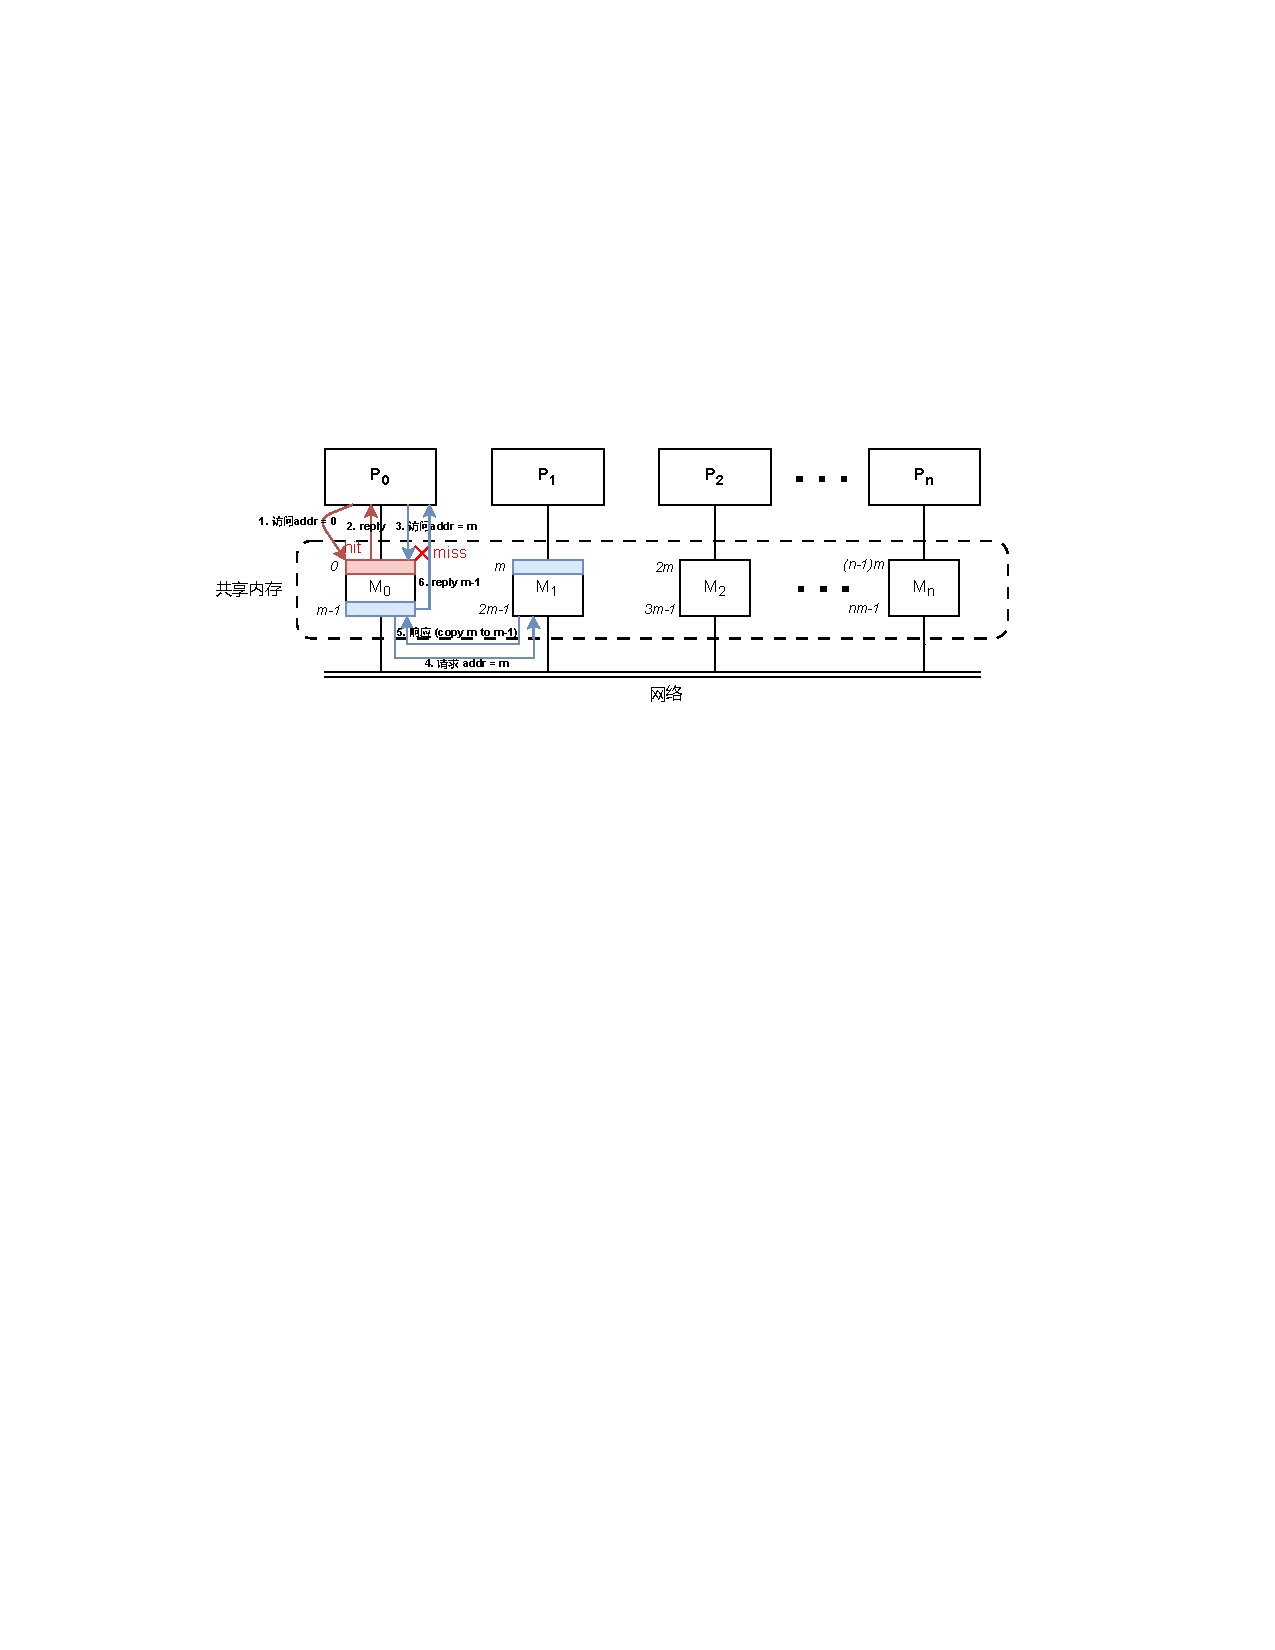
\includegraphics[width=\textwidth]{Img/shared-memory.pdf}
    %     \bicaption{\enspace 软件分布式共享内存}{\enspace shared memory principle}
    %     \label{fig:sharedmemory}
    % \end{figure}

    \subsection{实现层次}\label{sec:implementations}
    软件 DSM 系统实现方式灵活,可以在系统软件(操作系统或编译器)、运行时库、语言等层次上实现。
    \begin{itemize}
        \item \textbf{基于操作系统修改的软件DSM系统}:
              早期的软件 DSM 系统如 IVY\citep{likai1988ivy} ,Munin\citep{bennett1990munin}等通过依赖或修改系统软件来实现共享虚拟内存抽象和一致性管理。
              IVY 通过修改操作系统中的内存管理模块(Memory Management Unit, MMU)来监测远程访问,当处理机访问非本地页时,将触发缺页中断,并由 MMU 向远端取页;
              Munin 建立在 V 内核(V kernel)之上,依赖预处理器来检测用户对共享数据的注释,以便对不同类型的数据执行不同的一致性机制。这些方案由于需要系统软件支持导致可移植性差。

        \item \textbf{基于用户库形式软件 DSM 系统}:
              以用户库形式提供给开发者的全软件 DSM 系统是更为常见的实现。
              通过操作系统接口检测缺页异常并处理。系统初始化时使用 mmap() 建立共享虚拟内存与本地内存的映射,并通过 mprotect() 修改共享页权限。
              越权访问时,操作系统产生段违例信号(SIGSEGV),由预先注册的信号处理程序捕获并完成远程取数和权限授予。
              此类方案完全在用户空间运行,无需修改硬件或系统软件,仅依赖节点间通信能力,可移植性强。典型系统包括 TreadMarks、CRL、OpenSHMEM 及 JIAJIA。

        \item \textbf{基于语言或语言扩展级别的 DSM 系统}:
              语言或语言扩展级别的 DSM 系统在高性能计算社区发展为分区全局地址空间(PGAS)语言,通过扩展现有语言规范提供分布式共享内存编程模型,
              适合 Exascale 规模高性能并行计算。典型代表包括面向 Fortran 的 Coarray Fortran~\citep{numrich1998coarrayfortran, coarryfortran2}、
              面向 Java 的 Titanium~\citep{Yelick1998Titanium}、
              面向 C 的 UPC~\citep{bonachea2013UPC}(Unified Parallel C)以及面向 C++ 的 UPC++~\citep{bachan2019upc++}。
              与传统 DSM 系统的区别在于显式远程数据访问,程序员需明确指定数据来源。实现上依赖编译器和通信中间件层(如 GASNet~\citep{Bonachea2018GASNetEX})支持。
              GASNet 包含核心接口(Core API)和扩展接口(Extended API),前者直接实现于网络架构,后者独立于网络硬件,支持跨网络迁移。
    \end{itemize}

    \begin{figure}
        \centering
        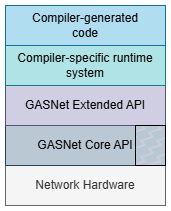
\includegraphics[width=0.3\textwidth]{Img/GASNet.png}
        \bicaption{\enspace GASNet 层系统图}{\enspace GASNet layer disgram}
        \label{fig:GASNET}
    \end{figure}

    \subsection{通信机制}
    软件 DSM 系统依赖底层的消息传递机制来实现上层的虚拟共享抽象。不同网络环境和协议实现的消息传递机制在通信流程和开销上展现出显著差异。

    为了追求更高的性能和可扩展性,传统 DSM 系统通常更倾向于采用低延迟的 UDP。在软件 DSM 系统的典型实现中,通常利用 SIGIO 信号来实现异步I/O通知,当 SIGIO 信号到达时,将导致当前执行被中断,转而执行相应的信号处理程序,之后再恢复原先的执行状态。

    RDMA 网络为现代软件 DSM 系统通信提供双重性能优势。一方面,高带宽、低延迟的特性极大的降低了通信传输延迟;另一方面,通过硬件直接访问内存,绕过内核协议栈,显著降低了协议处理和上下文切换带来的额外延迟。

    \subsection{内存一致性模型}
    内存一致性模型本质上是内存系统与并行程序之间的约定,它限制了系统可以执行内存访问的顺序。不同的内存一致性模型对访问顺序施加的限制的强弱程度不同,具体选择取决于对系统的性能要求和编程复杂度的权衡。维护内存一致性是软件 DSM 系统的关键问题,核心在于何时以及如何传播对共享内存的更新。

    \begin{itemize}
        \item \textbf{严格一致性模型(Strict Consistency):} 严格一致性模型要求任何一次读操作总是返回最近一次对相同对象的写入结果,实现需要全局时钟同步和零通信延迟的理想条件。

        \item \textbf{顺序一致性(Sequential Consistency):} 顺序一致性是最直观的内存一致性模型,最早由 Lamport 形式化定义,要求系统中所有进程对共享数据的操作必须呈现出一个全局的顺序,同时每个进程内部的操作顺序必须与程序中给定的顺序保持一致。

        \item \textbf{处理器一致性(Processor Consistency):} 处理器一致性比顺序一致性弱,核心特性可以概括为以下两条规则:
              \begin{enumerate}[label=\arabic*.]
                  \item 每个处理器内部发出的所有写操作必须以程序中的顺序被其他处理器观察到。
                  \item 对于同一内存地址,所有处理器都必须看到相同的写顺序;对于不同地址的写操作,各处理器可以看到的顺序不完全一致。
              \end{enumerate}

        \item \textbf{TSO(Total Store Order)}是一种特殊的处理器一致性,它通过允许同一处理中后续的读操作可以在写操作完成前提前执行,进一步隐藏了写入延迟,以提升性能。

        \item \textbf{弱一致性(Weak Consistecny):} 弱一致性模型的核心机制在于区分同步操作与普通访存操作,
              开发者通过显式的同步操作保护共享内存的写入,确保多个处理器对同一共享单元的写操作互斥,
              适用于对性能要求较高且数据一致性可容忍一定延迟更新的场景。

              \begin{figure}[!htbp]
                  \centering
                  \begin{subfigure}[b]{0.8\textwidth}
                      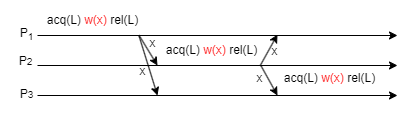
\includegraphics[width=\textwidth]{Img/eager-release-consistency.png}
                      \caption{急切更新释放一致性}
                      \label{fig:eager-release-consistency}
                  \end{subfigure}
                  \\
                  \begin{subfigure}[b]{0.8\textwidth}
                      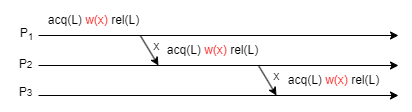
\includegraphics[width=\textwidth]{Img/lazy-release-consistency.png}
                      \caption{懒惰更新释放一致性}
                      \label{fig:lazy-release-consistency}
                  \end{subfigure}

                  \bicaption{\enspace 急切更新释放一致性 vs 懒惰更新释放一致性}{\enspace Eager release consistency vs Lazy release consistency}
                  \label{fig:oaspl}
              \end{figure}

        \item \textbf{释放一致性(Release Consistency):} 释放一致性的核心思想是把弱一致性中的同步操作进一步划分为获取操作(acquire)和释放操作(release)。只在特定的释放操作时才传播对共享内存的更新以保证数据一致性,而不是在每次访问共享内存时都强制同步。

        \item \textbf{懒惰更新释放一致性(Lazy release Consistency):} 懒惰更新释放一致性将更新传播的目的地范围限制为下一个获取锁的节点。这进一步减少了系统中通信消息的数量。
              下图说明懒惰更新释放一致性与急切释放一致性的通信比较。

        \item \textbf{域一致性(Scope Consistency):} 域一致性引入了一致性域(consistency scope)的概念,可以简单地将一致性域视为由锁保护的临界区。
              通过这一概念隐式地建立起共享内存对象与同步对象之间的关联,进而限制每次传播的共享内存对象更新的范围,有效降低了通信数据量。

        \item \textbf{单项一致性(Entry Consistency):} 单项一致性最早由 Midway 系统提出。开发者需要显示建立共享变量与同步变量之间的关联,对每一个共享变量的访问都需要由关联的同步变量来保护。具体而言,当获取同步变量(acquire)时,仅传播与同步变量关联的共享变量的更新。
    \end{itemize}

    \section{软件分布式共享内存系统 JIAJIA}
    \subsection{设计架构}
    \begin{figure}[!htbp]
        \centering
        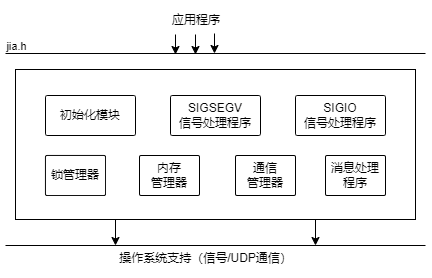
\includegraphics[width=\textwidth]{Img/JIAJIA-design.png}
        \bicaption{\enspace JIAJIA 设计架构}{\enspace JIAJIA design architecture}
        \label{fig:JIAJIA-design}
    \end{figure}
    JIAJIA 是一个国产软件 DSM 系统,以页为共享粒度,在物理分离的内存上提供逻辑共享的虚拟内存。JIAJIA 以用户库的形式提供给开发人员,开发人员可以使用 jia.h 头文件提供的接口编写采用分布式共享内存范式的并行程序,并使用 .jiahosts 配置文件设置参与分布式系统的节点组成。程序运行时,JIAJIA系统将会拷贝应用程序和配置文件到所有参与节点,随后并行执行协同完成任务。图~\ref{fig:JIAJIA-design} 显示了JIAJIA系统所包含的核心模块。

    \begin{enumerate}[label=\arabic*.]
        \item \textbf{初始化模块。}初始化模块用于对整个系统进行准备操作(见图~\ref{fig:JIAJIA-init}),负责加载配置文件(.jiahosts,.jiaconfig)以及初始化各个模块。
              \begin{figure}[!htbp]
                  \centering
                  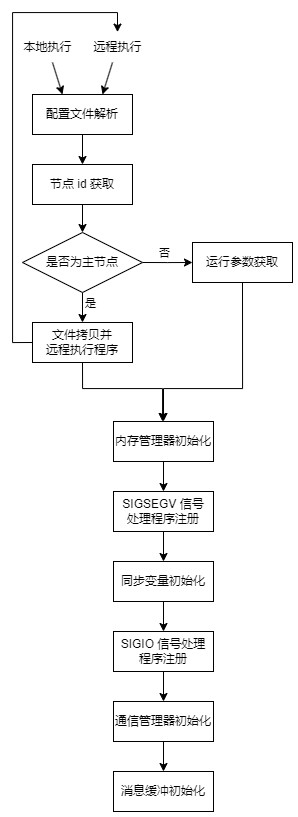
\includegraphics[width=0.6\textwidth]{Img/JIAJIA-init.png}
                  \bicaption{\enspace JIAJIA 初始化模块}{\enspace JIAJIA initialization module}
                  \label{fig:JIAJIA-init}
              \end{figure}

        \item \textbf{内存管理器。} JIAJIA 采用 NUMA 结构,是一个基于宿主(home-based)的系统,每个共享页都有对应的宿主节点核心包含三个数据结构:用于记录本地分配的共享页的目录(home),用于记录缓存页状态的缓存目录(cache),用于记录全部共享页的页目录(page)。JIAJIA 的内存组织如~\ref{fig:JIAJIA-memory}所示。
              \begin{figure}[!htbp]
                  \centering
                  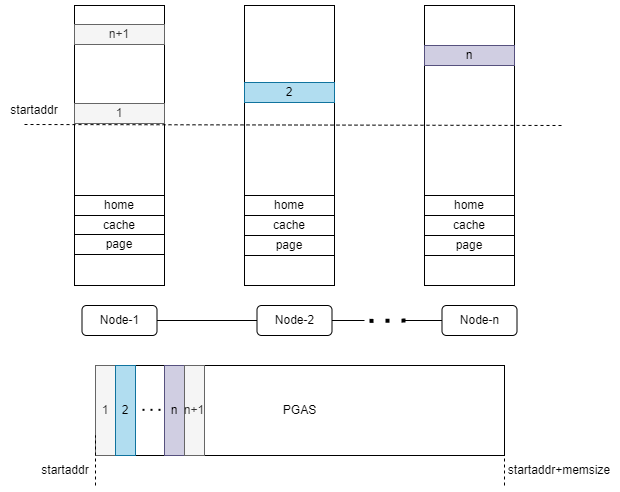
\includegraphics[width=0.65\textwidth]{Img/JIAJIA-memory.png}
                  \bicaption{\enspace JIAJIA 内存组织}{\enspace JIAJIA memory structure}
                  \label{fig:JIAJIA-memory}
              \end{figure}

        \item \textbf{SIGSEGV 信号处理程序。} JIAJIA 系统中任何节点都可以透明地访问任一共享内存位置。这一机理利用了操作系统的信号机制:当应用程序试图访问无权限内存时,将触发段违例信号(SIGSEGV),操作系统将捕获该信号并将其发送给预设的 SIGSEGV 信号处理程序。该程序将完成对本地内存的授权或对远程内存的取页操作。如图~\ref{fig:JIAJIA-access}所示。
              \begin{figure}[!htbp]
                  \centering
                  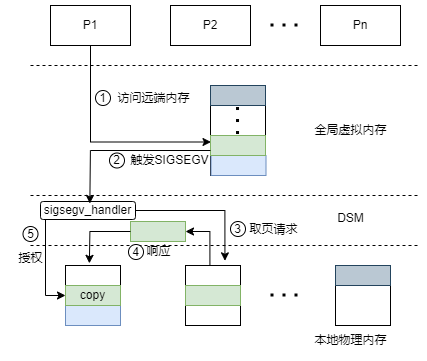
\includegraphics[width=0.65\textwidth]{Img/jiajia-access.png}
                  \bicaption{\enspace JIAJIA 访问远端内存}{\enspace JIAJIA }
                  \label{fig:JIAJIA-access}
              \end{figure}

        \item \textbf{通信管理器。} JIAJIA 使用通信管理器记录并管理发送和接收的套接字描述符。详见~\ref{chap:sdsm:sec:sigio}小节。

        \item \textbf{消息处理程序。} JIAJIA 底层基于消息传递机制,消息处理程序主要负责处理接收到的本地或远程消息,并根据消息类型执行相应的操作。如图~\ref{fig:JIAJIA-message-handle}。图~\ref{fig:JIAJIA-message-types}展示了JIAJIA中存在的消息类型。
              \begin{figure}[!htbp]
                  \centering
                  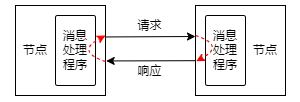
\includegraphics[width=0.50\textwidth]{Img/message-handler.png}
                  \bicaption{\enspace JIAJIA 底层消息传递机制}{\enspace JIAJIA underlying message passing mechanism}
                  \label{fig:JIAJIA-message-handle}
              \end{figure}

              \begin{figure}[!htbp]
                  \centering
                  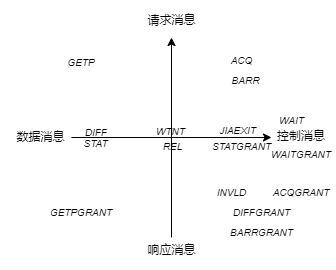
\includegraphics[width=0.50\textwidth]{Img/message-types.png}
                  \bicaption{\enspace JIAJIA 消息类型}{\enspace JIAJIA message types}
                  \label{fig:JIAJIA-message-types}
              \end{figure}

        \item \textbf{锁管理器。} 锁管理器主要负责同步变量的分配管理。JIAJIA 支持两种同步变量:锁(lock)和屏障(barrier)。开发者可以分别通过 jia\_lock 和 jia\_barrier 来请求锁或屏障的授权。对于锁同步变量,锁管理器维护一个先入先出队(FIFO)队列,按请求顺序依次授予锁权限;对于屏障同步变量,锁管理器通过计数器判断所有节点是否抵达相同位置,并在全部到达后统一授予继续运行的权限。
    \end{enumerate}

    \subsection{基于锁的缓存一致性协议}
    在内存一致性模型方面,JIAJIA 采用域一致性模型,并实现了一种基于锁的缓存一致性协议。该协议支持写失效的传播策略,并利用多写协议来避免假共享。

    JIAJIA 使用同步变量将应用程序分割为一个个一致性域(或称为临界区间),每到达一个同步原语都代表一个旧临界区间的结束,以及新临界区间的开始,见图~\ref{fig:JIAJIA-scopes}。
    在旧临界区间(如scope1)结束时,将传播在该临界区中对共享页做的修改给相应的宿主节点。
    JIAJIA 基于锁的一致性协议的特点是它将一个临界区域内对共享页的修改信息(写通知,write-notice)与锁绑定,
    write-notice 记录了修改页的地址,获取锁的处理机将根据锁管理器中的 write-notice 得知哪些页面已被其他处理机修改。
    在处理临界区嵌套情况时,JIAJIA 使用堆栈结构来记录锁的嵌套,获取锁时压栈,释放锁时弹栈,弹栈时将把栈顶锁的 write-notice 合并到下一层。

    \begin{figure}[!htbp]
        \centering
        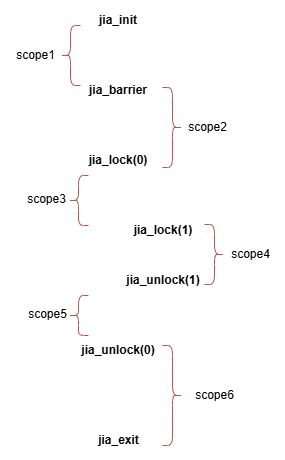
\includegraphics[width=0.50\textwidth]{Img/JIAJIA-scope.png}
        \bicaption{\enspace JIAJIA 一致性域}{\enspace JIAJIA consistency scope}
        \label{fig:JIAJIA-scopes}
    \end{figure}

    \section{RDMA 技术介绍}
    远程直接内存访问(Remote Direct Memory Access, RDMA)技术是一种应用于高性能计算领域的网络通信协议,支持远程直接读写异地内存,而无需双方操作系统甚至 CPU 的介入。
    如图~\ref{fig:DMA-RDMA}所示,RDMA 可视作直接内存访问(Direct Memory Access, DMA)在分布式系统上的扩展,把直接访问内存的范围从单机内存扩展到了远端内存。
    \begin{figure}[!htbp]
        \centering
        \begin{subfigure}[b]{0.40\textwidth}
            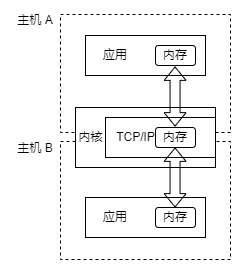
\includegraphics[width=\textwidth]{Img/TCPIP.png}
            \caption{TCP/IP 通信}
            \label{fig:TCPIP}
        \end{subfigure}%
        ~~~~~% add desired spacing
        \begin{subfigure}[b]{0.40\textwidth}
            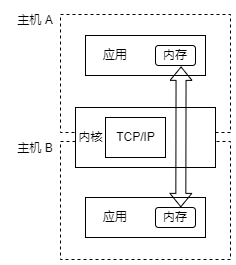
\includegraphics[width=\textwidth]{Img/RDMA.png}
            \caption{RDMA 通信}
            \label{fig:RDMA}
        \end{subfigure}
        \bicaption{\enspace DMA 与 RDMA 的比较}{\enspace }
        \label{fig:DMA-RDMA}
    \end{figure}

    RDMA(Remote Direct Memory Access)是一种针对传统 TCP/IP 网络协议栈(图~\ref{fig:TCPIP})高延迟和高 CPU 开销问题的优化方案。
    在传统的 TCP/IP 通信模式下,跨机器的应用通信需要经历多个数据拷贝过程:
    首先,应用数据需从用户空间拷贝至内核空间,然后由 TCP/IP 协议栈进行封装,接着传输至驱动层,最终写入网卡缓存并发送到远端。
    这一过程中涉及复杂的协议处理和多次数据拷贝,导致 CPU 负担沉重,影响通信效率。

    相比之下,RDMA 通信模式(图~\ref{fig:RDMA})通过硬件直接访问内存,实现数据传输,无需拷贝至内核空间,同时由硬件完成协议处理并将数据传输至远端设备。
    RDMA 主要具备以下三大核心特性:

    \begin{enumerate}[label=\arabic*.]
        \item \textbf{零拷贝}(Zero-Copy)。数据可以直接从发送端用户空间传输到接收端用户空间,无需在内核空间与用户空间之间进行多次拷贝,从而减少延迟,提高吞吐量。
        \item \textbf{内核旁路}(Kernel Bypass)。RDMA 采用用户态驱动(如 Verbs API)直接控制网卡,绕过传统 TCP/IP 协议栈,避免内核态的数据封装、解析及中断处理,从而减少上下文切换的开销。
        \item \textbf{CPU 卸载}(CPU Offloading)。RDMA 通过两种方式降低 CPU 负担:
              \begin{itemize}
                  \item 网络协议处理(如报文组装、分片重组、流量控制等)完全由网卡硬件执行,而非 CPU 处理;
                  \item 采用 RDMA 内存语义(如 RDMA Read/Write)进行数据传输时,远端 CPU 无需参与,从而进一步减少计算资源的占用。
              \end{itemize}
    \end{enumerate}

    \subsection{RDMA 通信模式与通信原语}
    RDMA 使用 QPs 作为通信基本单元行通信,QPs 的类型决定了 RDMA 通信链路的模式。见图~\ref{fig:rdma-queue-pairs}。
    \begin{figure}[!htbp]
        \centering
        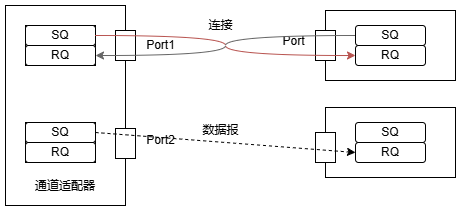
\includegraphics[width=\linewidth]{Img/QueuePairs.png}
        \bicaption{\enspace RDMA 队列对}{\enspace RDMA Queue Pairs}
        \label{fig:rdma-queue-pairs}
    \end{figure}

    QPs 的类型可以根据是否建立连接以及是否可靠来划分。因此 RDMA 相应的支持四种通信链路模式即四种类型的 QPs,分别是:可靠连接(RC)、不可靠连接(UC)、不可靠数据报(UD)、可靠数据报(RD)。其中 RC 模式和 UC 模式均是点对点通信,在通信之前需要在节点之间建立一对一的连接,区别是RC 模式提供可靠的传输服务,而 UC 模式无法确保数据包按序、无丢失交付,可靠性需要由上层协议来保证。UD 模式类似于 UDP ,特点是面向无连接通信、支持多播、以及单个消息大小受限于路径最大传输单元(path MTU)。RD 模式当前并未有实现支持。

    RDMA 支持两类通信原语即所谓的动词(Verbs),双向动词和单向动词。双向动词又称为消息语义,包含 SEND 和 RECV ,适合传输控制消息;单向动词又称为内存语义,包含 RDMA Read 、RDMA Write 和 RDMA 原子操作(Fetch-and-Add/FAA,Compare-and-Swap/CAS),RDMA Read 和 RDMA Write 适合大量数据传输,RDMA 原子操作适合需要强一致性保证和低延迟并发控制的场景。表~\ref{tab:mode-verbs}展示了 RDMA 通信模式和通信原语的支持关系。

    \begin{table}[!htbp]
        \footnotesize% fontsize
        \setlength{\tabcolsep}{4pt}% column separation
        \renewcommand{\arraystretch}{1.5}% row space 
        \centering
        \begin{tabular}{lcccc}
            \hline
            %\multicolumn{num_of_cols_to_merge}{alignment}{contents} \\
            %\cline{i-j}% partial hline from column i to column j
               & Send/Recv  & RDMA Write & RDMA Read  & RDMA Atomic \\
            \hline
            RC & \checkmark & \checkmark & \checkmark & \checkmark  \\
            UC & \checkmark & \checkmark & \times     & \times      \\
            UD & \checkmark & \times     & \times     & \times      \\
            \hline
        \end{tabular}
        \bicaption{\enspace RDMA 通信模式与通信原语的关系}{\enspace Relation between RDMA communication mode and verbs}% caption
        \label{tab:mode-verbs}
    \end{table}

    \subsection{RDMA 通信流程}
    不同的 RDMA Verbs 在通信时有不同的执行的流程,以下是对几种常见 Verbs 通信流程的介绍。
    \begin{enumerate}[label=\arabic*.]
        \item Send/Recv 通信流程

              \begin{figure}[!htbp]
                  \centering
                  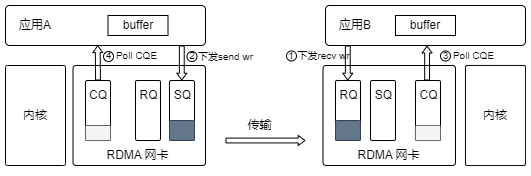
\includegraphics[width=\linewidth]{Img/RDMA-Send.png}
                  \bicaption{\enspace Send/Recv 通信流程图}{\enspace Send/Recv Communication Flow Diagram}
                  \label{fig:rdma-send}
                  {\small Note: 不同 RDMA 实现对于通信硬件设备有不同的名称,本文统称为 RDMA 网卡}
              \end{figure}
              图~\ref{fig:rdma-send}显示了左侧应用A尝试利用 Send 向远程应用 B 发送数据(其中省略了RDMA 网卡访存的操作)的流程。为了实现这一通信,将执行如下步骤:
              \begin{itemize}
                  \item 应用 B 首先向 RQ 下发接收工作请求,其中包含了对 RDMA 网卡的提示,网卡将据此把接收到的数据放到内存中的指定位置。
                  \item 应用 A 向 SQ 中下发发送工作请求,
                        本地网卡将根据 SQE 从应用 A 的内存取出数据并发往远端。
                  \item 远端 RDMA 网卡接收到数据后根据RQ 中的提示将数据放入应用 B 的相应内存中。
                  \item 网卡将请求的执行状态放入 CQ 中,应用可通过轮询得到上一个请求的结果。
              \end{itemize}

              从上述流程中可以看出,Send/Recv 操作需要接收方 CPU 的参与。而且需要注意的是,在不同链路模式下,CQE 产生的时机会有所不同。UD模式下,在将数据放入网络后便产生 CQE;而RC模式下,可能需要等到远端发回确认消息后,才会产生 CQE 。

        \item RDMA Read 通信流程
              \begin{figure}[!htbp]
                  \centering
                  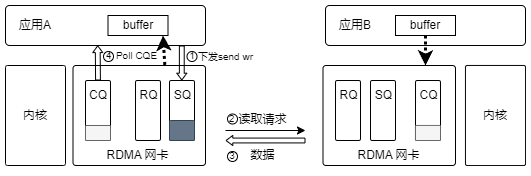
\includegraphics[width=\linewidth]{Img/RDMA-Read.png}
                  \bicaption{\enspace RDMA Read 通信流程图}{\enspace RDMA Read Communication Flow Diagram}
                  \label{fig:rdma-Read}
              \end{figure}

              RDMA Read 用于直接读取远端内存。如~\ref{fig:rdma-Read}所示,其执行流程如下:
              \begin{itemize}
                  \item 应用 A 向 SQ 中下发读取工作请求。
                  \item 本地网卡根据 SQ 中的 WQE 向远端发送读取请求包。
                  \item 远端网卡接收到读取请求包后,根据包中携带的信息,读取应用 B 相应位置的内存,并发回数据。
                  \item 本地网卡接收到数据,根据 WQE 的信息将数据存入应用 A 的内存,并向 CQ 中存入CQE。
                  \item 应用通过轮询 CQ 获得 CQE,从中获取上一个请求的完成情况。
              \end{itemize}

        \item RDMA Write 通信流程
              \begin{figure}[!htbp]
                  \centering
                  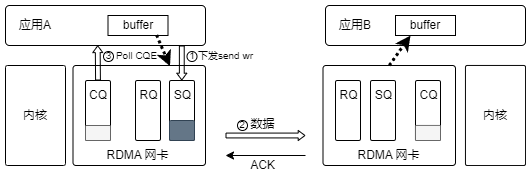
\includegraphics[width=\linewidth]{Img/RDMA-Write.png}
                  \bicaption{\enspace RDMA Write 通信流程图}{\enspace RDMA Write Communication Flow Diagram}
                  \label{fig:rdma-Write}
              \end{figure}

              RDMA Write 用于直接写入远端内存。如~\ref{fig:rdma-Write}所示,其执行流程如下:
              \begin{itemize}
                  \item 应用 A 向 SQ 中下发写入工作请求。
                  \item 本地网卡根据 SQ 中的 WQE 中的提示读取本地内存,组装数据包发往远端。
                  \item 远端网卡收到数据包后解析得到数据目的地址,将数据写入相应位置后返回 ACK 。
                  \item 本地网卡根据返回的 ACK 信息生成 CQE,并将其放入 CQ。
                  \item 应用通过轮询 CQ 获得 CQE,从中获取上一个请求的完成情况。
              \end{itemize}
    \end{enumerate}

    通过上述的流程分析可得出 RDMA Verbs 的如下特征,双向动词 Send/Recv 需要远端 CPU 参与提前下发接收请求,类似于传统的消息传递模型,而单向动词 RDMA Read、RDMA Write 可以绕过远端CPU,直接读取或写入指定的内存位置。
    无论是 Send 还是 RDMA Read、RDMA Write 都将向 SQ 中下发发送工作请求,网卡将根据其中指定的操作码(Opcode)字段来区分,RQ 仅在 Send/Recv 时使用。相比于RDMA Read, Send/Recv 和 RDMA Write 不需要网卡发回数据包,因此在传输小数据报时,RDMA Write 和 Send/Recv 的传输延迟大约是 RDMA Read 的一半~\citep{kalia2014herd}(见图~\ref{fig:RDMA-Verbs-Latency})。
    \begin{figure}[!htbp]
        \centering
        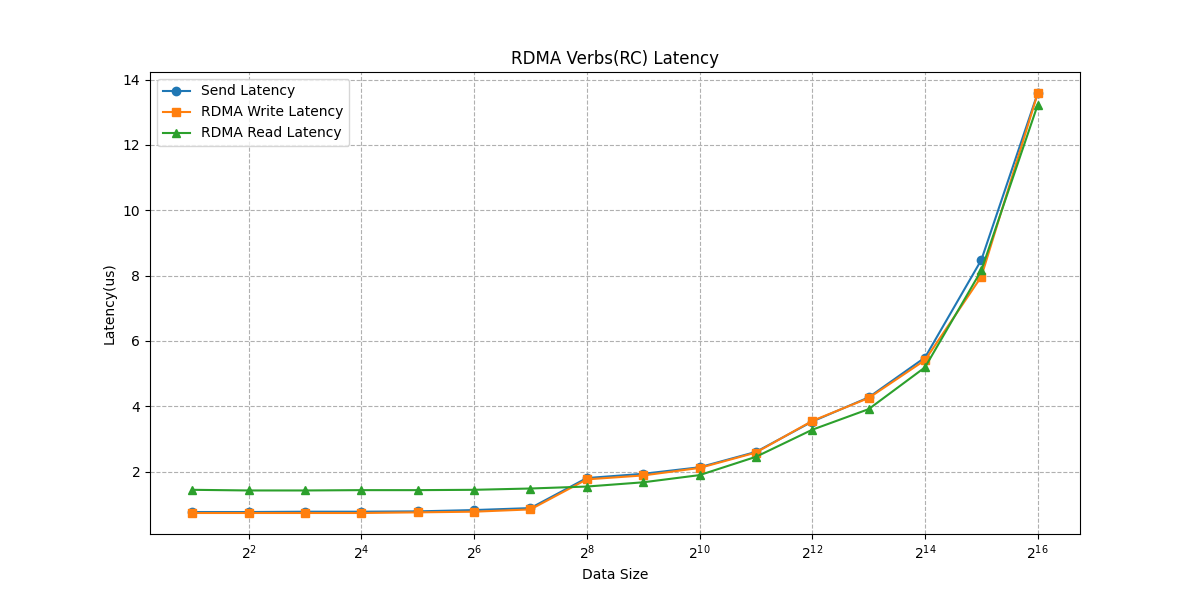
\includegraphics[width=\linewidth]{Img/verbs-latency.png}
        \bicaption{\enspace RDMA Verbs 通信延迟比较}{\enspace Comparison of Communication Latency of RDMA Verbs}
        {\small Note: 在Mellanox ConnectX-3 Pro 网卡可靠连接下的测试}
        \label{fig:RDMA-Verbs-Latency}
    \end{figure}

    \subsection{RDMA 实现与通信基础库}
    \textbf{RDMA 实现架构}:RDMA 有多种不同的实现架构,包括无限带宽(InfiniBand,IB)、基于融合以太网的RDMA(RDMA over Converged Ethernet,RoCE)、互联网广域 RDMA 协议(internet Wide Area RDMA Protocol,iWARP)等。它们之间的区别如图~\ref{fig:RDMA-Implementations}所示:
    \begin{figure}[!htbp]
        \centering
        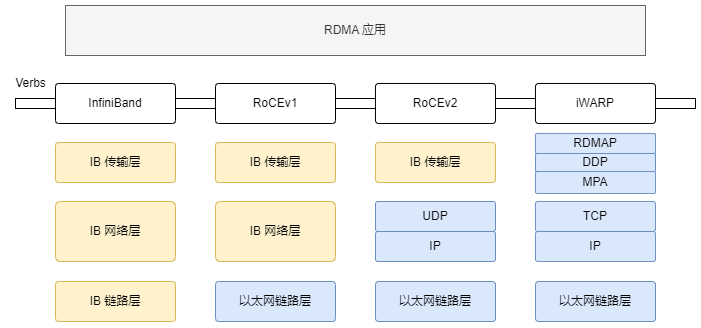
\includegraphics[width=\linewidth]{Img/RDMA-Implementation.png}
        \bicaption{\enspace RDMA 不同实现架构}{\enspace Different RDMA Implementation Architectures}
        \label{fig:RDMA-Implementations}
    \end{figure}

    \begin{enumerate}[label=\arabic*.]
        \item InfiniBand 是由InfiniBand 贸易协会(IBTA)定义的用于高性能计算网络通信标准,其设计目标在于为大规模并行计算系统提供超低延迟和高带宽的数据传输解决方案。该技术采用分层协议结构,通过采用独立于TCP/IP 的全新网络协议栈,有效规避了操作系统协议栈带来的性能损耗。在物理层实现上,IB 网络构建需要专用硬件基础设施,包括IB 交换机、IB 路由器,以及配置了Host Channel Adapter(HCA)的终端节点。这些架构特性使其在支持 RDMA 上展现出显著性能优势,目前在超级计算机集群、分布式存储系统以及人工智能训练平台等对网络性能要求严苛的场景下被广泛应用。
        \item RoCE 同样是由 IBTA 提出的在以太网上支持RDMA的协议,其核心目标是通过复用传统以太网硬件设施以降低 RDMA 技术的部署成本。目前包含两个版本RoCEv1和RoCEv2。RoCEv1 在以太网链路层(L2)实现了IB 传输层数据包的封装,通过以太网帧直接承载远程内存访问操作。但由于未引入IP层路由机制,其通信范围被限制在单一广播域内,仅支持同一子网或VLAN内的节点间数据传输,且需依赖无损以太网的优先级流量控制(PFC)技术以规避丢包风险。RoCEv2 通过利用UDP/IP协议栈封装IB传输层数据,即保留了 IB 传输层语义又增加了对路由功能的支持,从而突破RoCEv1 对子网的边界限制,使其成为更大规模部署的通用解决方案。
        \item iWARP 是互联网工程任务组(IETF)提出的在TCP/IP协议栈上实现远程直接内存访问(RDMA)的技术体系。该技术基于三层核心组件——从上层向下层依次是远程直接内存访问协议(Remote Direct Memory Access Protocol, RDMAP)、直接数据放置(Direct Data Placement, DDP)和标记协议数据单元对齐(Marker PDU Aligned Framing, MPA)。其中 RDMAP 负责提供零拷贝操作原语,DDP 解耦网络传输与内存语义映射,MPA负责保证 TCP 报文边界对齐。 由于 TCP 是面向连接的,iWARP 仅支持点对点可靠通信,缺乏对组播和广播的支持。
    \end{enumerate}

    上述三种不同的 RDMA 实现,由于在协议栈设计、硬件依赖及端到端传输机制等方面的不同,在性能、成本和扩展性上也存在差异。性能上,IB \text{>} RoCEv2 \text{>} iWARP(由高到低);部署成本上,iWARP \text{>} RoCEv2 \text{>} IB(由低到高);可扩展性上,iWARP \text{>} RoCEv2 \text{>} IB(由高到低);不过RDMA 网卡厂商为了应对异构网络环境,通常会通过灵活设计的硬件架构同时支持两种不同的架构,比如英伟达(NVIDIA)的ConnectX系列网卡兼容IB和RoCEv2双模式,而掣速科技(Chelsio)的T6系列网卡则同时支持 RoCEv2 和 iWARP。

    \textbf{RDMA 通信基础库}: 为了开发可以原生利用 RDMA 的应用,OpenFabrics 联盟推动实现了一组协议无关的统一软件编程接口,用户利用这些接口可以开发出在 IB、RoCE、iWARP架构上无缝移植的应用。其中通信传输方面涉及到两个核心用户空间库,\textbf{libibverbs} 和 \textbf{librdmacm}。
    % \begin{enumerate}[label=\arabic*.]
    %     \item \textbf{libibverbs} 是InfiniBand Verbs API的底层实现库,提供了对RDMA硬件的直接访问能力。核心功能包括设备操作、通信管理(QP管理,任务下发)、内存注册、完成处理等。
    %         \begin{table}[!htbp]
    %             \footnotesize% fontsize
    %             \setlength{\tabcolsep}{4pt}% column separation
    %             \renewcommand{\arraystretch}{1.5}% row space 
    %             \centering
    %             \begin{tabular}{|p{1.3cm}|p{4.5cm}|p{5.5cm}|p{3.7cm}|}
    %                 \hline
    %                 %\multicolumn{num_of_cols_to_merge}{alignment}{contents} \\
    %                 %\cline{i-j}% partial hline from column i to column j
    %                  & 准备 & 使用 & 销毁\\
    %                  \hline
    %                  \multirow{2}{*}{设备操作} &   ibv\_get\_device\_list, & ibv\_query\_device, ibv\_query\_port, & ibv\_close\_device \\
    %                  & ibv\_open\_device & ibv\_query\_gid, ibv\_query\_pkey & \\
    %                 \hline
    %                通信管理 & ibv\_create\_qp, ibv\_open\_qp & ibv\_post\_recv, ibv\_post\_send & ibv\_destroy\_qp \\
    %                 \hline
    %                 内存注册 & ibv\_alloc\_pd, ibv\_reg\_mr &  & ibv\_dealloc\_pd, ibv\_dereg\_mr \\
    %                 \hline
    %                 \multirow{2}{*}{完成处理} & ibv\_create\_cq, & ibv\_poll\_cq, ibv\_req\_notify\_cq, & ibv\_destroy\_cq, \\
    %                 & ibv\_create\_comp\_channel  & ibv\_get\_cq\_event, ibv\_ack\_cq\_events & ibv\_destroy\_comp\_channel \\
    %                 \hline
    %             \end{tabular}
    %             \bicaption{\enspace libibverbs 库核心接口}{\enspace libibverbs core API}% caption
    %             \label{tab:libibverbs-api}
    %         \end{table}    
    %     \item \textbf{librdmacm} 是一个 RDMA 通信管理库,为建立 RDMA 连接提供类似 Socket 的编程抽象,并对部分 libibverbs 的接口进行了包装。核心功能包括连接管理、事件处理、资源管理等。
    %         \begin{table}[!htbp]
    %             \footnotesize% fontsize
    %             \setlength{\tabcolsep}{4pt}% column separation
    %             \renewcommand{\arraystretch}{1.5}% row space 
    %             \centering
    %             \begin{tabular}{|p{1.3cm}|p{4.5cm}|p{5.5cm}|p{3.7cm}|}
    %                 \hline
    %                 %\multicolumn{num_of_cols_to_merge}{alignment}{contents} \\
    %                 %\cline{i-j}% partial hline from column i to column j
    %                  & 准备 & 使用 & 销毁\\
    %                  \hline
    %                  \multirow{7}{*}{连接管理} &   rdma\_create\_event\_channel, & 
    %                  rdma\_get\_cm\_event, rdma\_ack\_cm\_event  & rdma\_destroy\_event\_channel \\
    %                  &  & rdma\_event\_str  & \\
    %                  & rdma\_create\_id & rdma\_resolve\_addr, rdma\_resolve\_route  & rdma\_destroy\_id \\
    %                  &  & rdma\_connect, rdma\_disconnect  & \\
    %                  &  & rdma\_bind\_addr, rdma\_listen  & \\
    %                  &  & rdma\_accept, rdma\_reject  & \\
    %                 &  & rdma\_migrate\_id  & \\
    %                 \hline
    %                 \multirow{4}{*}{资源管理} & rdma\_create\_ep, rdma\_create\_qp & rdma\_post\_send, rdma\_post\_recv, & rdma\_destroy\_ep, \\
    %                 & rdma\_reg\_msgs & rdma\_post\_read, rdma\_post\_write & rdma\_destroy\_qp \\
    %                 &rdma\_reg\_read, rdma\_reg\_write & ... & \\
    %                 \hline
    %             \end{tabular}
    %             \bicaption{\enspace librdmacm 库核心接口}{\enspace librdmacm core API}% caption
    %             \label{tab:compiler}
    %         \end{table}   
    % \end{enumerate}

    \subsection{RDMA 通信 vs Socket 通信}
    套接字(Socket)API 是传统网络通信的核心编程接口,为TCP/IP协议栈提供了标准化的进程间通信机制。该接口通过抽象通信端点实现了跨主机的数据传输能力,每个套接字由本地IP地址与端口号组成的二元组唯一标识,并与对端地址共同构成完整的通信链路。在 UNIX/Linux 系统上,套接字是一类特殊的文件,通过文件描述符机制与其他输入/输出(I/O)资源共享相同的接口。这种设计遵循 "一切皆文件" 的哲学,使得网络通信可以像文件读写一样进行操作,例如可以使用 read、write系统调用来接收和发送数据。此外,文件描述符的多路复用技术(如 select、poll 和 epoll)同样可以用于同时管理多个套接字,以提高 I/O 处理的效率。

    根据传输层协议差异,套接字主要分为三种类型:基于TCP协议的流式套接字(stream socket)、基于UDP协议的数据报套接字(datagram socket)和绕过传输层的原始套接字(raw socket),见图~\ref{fig:Socket-Type}。
    \begin{figure}[!htbp]
        \centering
        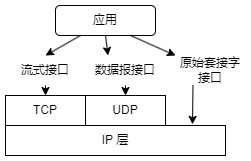
\includegraphics[width=0.35\linewidth]{Img/Socket-Type.png}
        \bicaption{\enspace 三种 Socket 类型}{\enspace The Three Socket Types}
        \label{fig:Socket-Type}
    \end{figure}
    在传统网络编程实践中,传输层协议的选择不仅决定socket的类型,还深刻影响整个通信子系统的设计,主要体现在连接管理、数据传输、错误处理等方面,这里对使用TCP/UDP两种最常用的传输层协议进行了比较。

    \begin{itemize}
        \item 连接管理:TCP是面向连接的协议,在数据传输前需要通过三次握手完成客户端和服务器的建连,客户端将使用 connect() 主动发起连接,而服务器需要调用 listen() 提前进入监听状态并调用 accept() 处理客户端连接,在通信结束双方使用 close() 断连;而 UDP 是无连接协议,无需建立和维护连接,应用程序可直接使用 sendto() 和 recvfrom() 进行通信。
        \item 数据传输:TCP采用字节流的方式传输数据,提供可靠、有序的数据传递;而 UDP采用数据报的形式进行传输,通过 sendto()/recvfrom() 对完成一个数据包的发送和接收。
        \item 错误处理:TCP 协议采用滑动窗口、超时重传和流量控制机制确保数据的可靠交付;而 UDP 传输的可靠性需要依赖应用层的确认和重传机制。
    \end{itemize}

    相比之下,RDMA 通信需要开发者深入了解底层网络协议与硬件特性。通信流程如下(以可靠连接为例):
    \begin{enumerate}[label=\textbf{步骤 \arabic*.}, leftmargin=0.5cm, align=left]
        \item \textbf{设备发现与初始化}
              \begin{itemize}
                  \item 通过\texttt{ibv\_get\_device\_list()}获取网卡设备列表,选择使用的设备(ibv\_device)。
                  \item 通过\texttt{ibv\_open\_device()}打开指定设备,获取设备上下文(ibv\_context)。
              \end{itemize}

        \item \textbf{资源隔离域构建与内存注册}
              \begin{itemize}
                  \item 通过\texttt{ibv\_alloc\_pd()}创建保护域以隔离RDMA资源(ibv\_pd)。
                  \item 通过\texttt{ibv\_reg\_mr()} 注册内存区域(ibv\_mr)。
              \end{itemize}

        \item \textbf{通信终端创建}
              \begin{itemize}
                  \item 通过\texttt{ibv\_create\_cq()}创建完成队列(ibv\_cq)。
                  \item 配置QP属性,并通过\texttt{ibv\_create\_qp()}创建QP(ibv\_qp)。
              \end{itemize}

        \item \textbf{连接建立操作}
              \begin{itemize}
                  \item 可选择采用传统Socket交换通信元数据,或采用 RDMA CM 建连。
              \end{itemize}

        \item \textbf{数据平面操作}
              \begin{itemize}
                  \item 构造工作请求,并指定选用的RDMA操作类型。
                  \item 通过\texttt{ibv\_post\_send()}提交工作请求至发送队列,
                  \item 轮询完成队列并获取完成事件,检验事件状态以判断请求完成情况
              \end{itemize}

        \item \textbf{资源回收操作}
              \begin{itemize}
                  \item 按拓扑逆序销毁队列对、完成队列、内存区域等对象。
                  \item 释放保护域并关闭设备。
              \end{itemize}
    \end{enumerate}
    图~\ref{fig:RDMA-structs}展示了 libibverbs 和 librdmacm 库核心数据结构之间的引用关系。在创建一个数据结构之前,需要首先完成其引用数据结构的创建。
    \begin{figure}[!htbp]
        \centering
        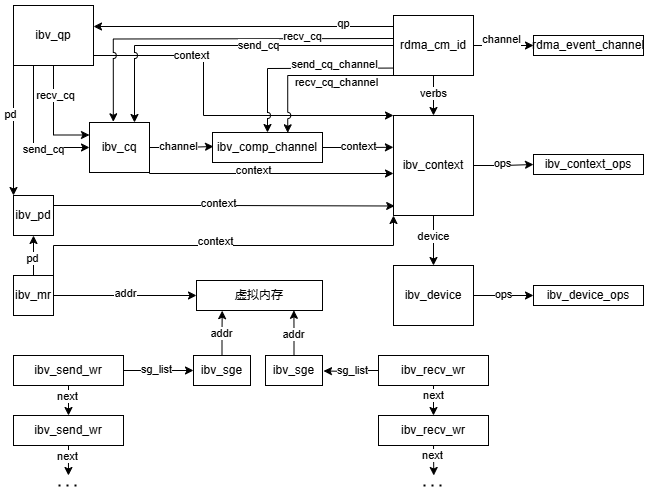
\includegraphics[width=\linewidth]{Img/RDMA-structs.png}
        \bicaption{\enspace RDMA 关键数据结构引用关系图}{\enspace The RDMA key data structure reference relationship diagram}
        \label{fig:RDMA-structs}
    \end{figure}



    \section{本章小结}
}
\chapter{多线程 M-JIAJIA 的设计与实现}\label{chap:MJIAJIA}{
    本章主要介绍 M-JIAJIA 的设计与实现,M-JIAJIA 在 JIAJIA 的基础上实现,并继承了域一致性模型,其主要优化集中在通信子系统。M-JIAJIA 采用分层模块化设计,解耦通信层和系统核心模块层,两个层之间通过消息队列进行通信。通信层支持 UDP 通信和 RDMA 通信两种方案,并采用多线程流水化技术优化通信效率。

    \section{设计概览}
    \begin{figure}[!htbp]
        \centering
        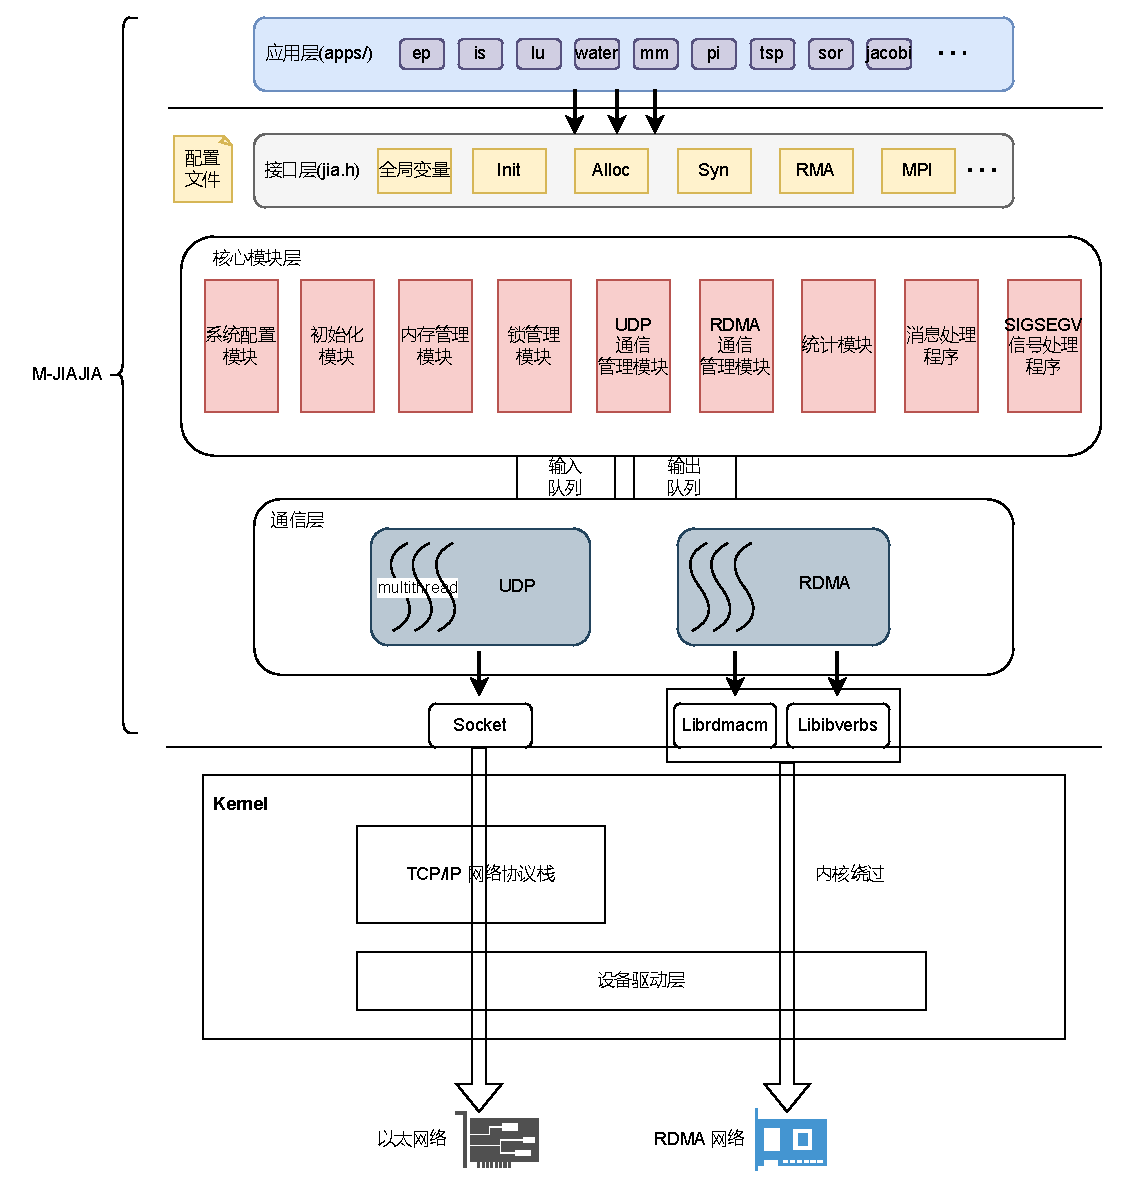
\includegraphics[width=1.0\textwidth]{Img/MJIAJIA系统框架图.drawio.pdf}
        \bicaption{M-JIAJIA系统框架图}{M-JIAJIA Sytem Framework Diagram}
        \label{fig:system-arch}
    \end{figure}
    M-JIAJIA 的整体架构如图~\ref{fig:system-arch} 所示。从上到下依次是应用层、接口层、核心模块层、通信层。其中应用层主要包含了 M-JIAJIA 系统的并行测试程序(将在~\ref{chap:experiments}章节做进一步介绍)。本章节剩余部分将主要介绍接口层、核心模块层、通信层的设计与实现。

    \section{函数接口设计}
    M-JIAJIA 在函数接口设计上保持了对 JIAJIA 系统接口的兼容,提供列表~\ref{lst:jia-interface}所示 C 语言的编程接口。主要包括全局变量、系统操作、内存操作、同步操作、消息传递接口、和 RDMA(远程内存访问) 接口等。
    \begin{lstlisting}[style=CStyle, caption={M-JIAJIA C 接口总览}, label={lst:jia-interface}]
/* 全局变量 */
extern int jiahosts;
extern int jiapid;
/* 系统操作 */
void jia_init(int argc, int argv);
void jia_exit();
/* 内存操作 */
unsigned long jia_alloc(int totalsize);
unsigned long jia_alloc2(int totalsize, int blocksize);
unsigned long jia_alloc2p(int totalsize, int starthost);
unsigned long jia_alloc3(int totalsize, int blocksize, int starthost);
unsigned long jia_alloc4(int totalsize, int *blocks, int n, int starthost);
unsigned long jia_alloc_random(int totalsize);
unsigned long jia_alloc_array(int totalsize, int *array, int n);
void jia_free(void *addr);
/* 同步操作 */
void jia_lock(int lockid);
void jia_unlock(int lockid);
void jia_barrier();
void jia_wait();
/* 消息传递接口 */
void jia_send(char *buf, int len, int topid, int tag);
int jia_recv(char *buf, int len, int frompid, int tag);
    \end{lstlisting}

    \subsection{配置文件}
    M-JIAJIA 程序采用单程序多数据(Single Program Multiple Data, SPMD)并行计算模式,运行时系统将同一程序动态部署到分布式计算节点上协同执行。
    系统向开发者提供两个配置文件:.jiahosts 和 .jiaconfig,分别用于指定运行的主机和JIAJIA系统的配置。
    同时在JIAJIA系统运行时,每台主机会根据在.jiahosts中的序号拥有自己唯一的jia\_pid.

    \subsection{系统操作}\label{sec:init}
    系统操作接口包含 jia\_init 和 jia\_exit 两个必要接口。jia\_init 用于完成系统的初始化工作,将调用核心层中的初始化模块(图~\ref{fig:mjiajia-init})。
    \begin{figure}[!htbp]
        \centering
        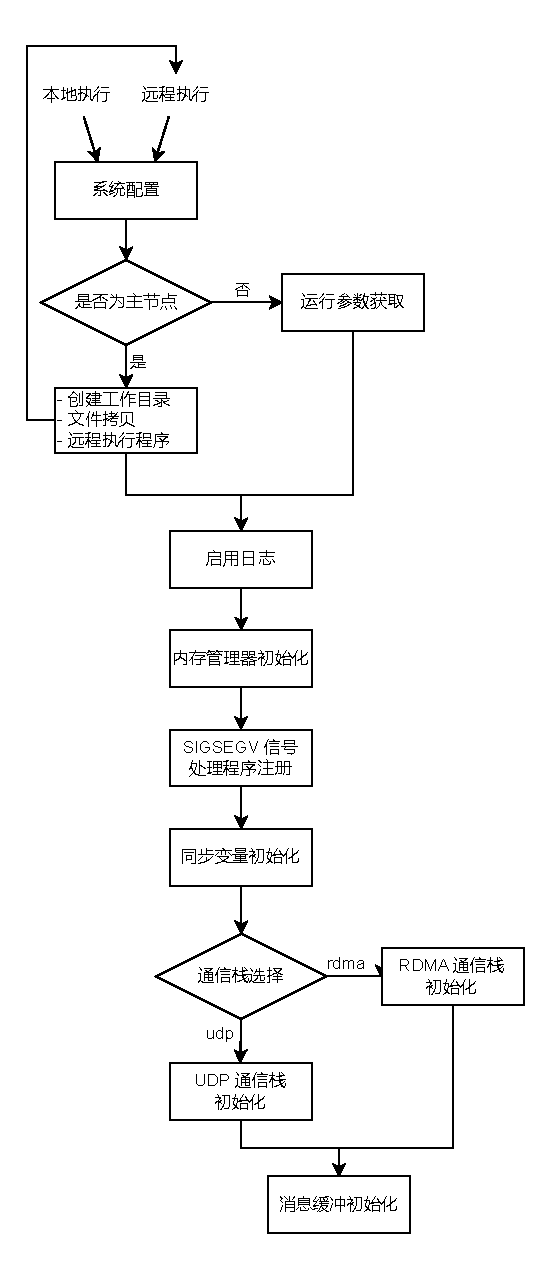
\includegraphics[width=0.6\textwidth]{Img/M-JIAJIA-初始化模块.drawio.pdf}
        \bicaption{M-JIAJIA 初始化模块}{M-JIAJIA initial module}
        \label{fig:mjiajia-init}
    \end{figure}
    相比于 JIAJIA 的初始化模块,M-JIAJIA 做了如下架构改进以满足系统的灵活和可维护性要求:
    \begin{itemize}
        \item 重构配置文件解析逻辑,只依赖 .jiahosts 文件中提供的IP地址、用户名和密码三元组,计算节点之间的连通性由开发者保证。
        \item 引入远程工作目录概念,初始化阶段将为远程节点创建程序工作目录jianode,所有从节点的进程都会在工作目录 jianode 下执行。
        \item 动态初始化网络通信栈,根据系统配置自动选择并初始化 UDP 或 RDMA 通信栈。
    \end{itemize}

    jia\_exit 用于收集所有远程节点的统计信息,并在释放系统资源后退出。
    \subsection{同步操作}
    M-JIAJIA 提供两种同步原语 jia\_lock 和 jia\_barrier 和一种等待原语 jia\_wait,
    用于保证 JIAJIA系统访问共享变量的一致性以及操作的同步性。

    \subsection{消息传递接口}
    消息传递接口用于分布式编程中节点之间的显式通信,M-JIAJIA 支持类消息传递的接口 jia\_send 和 jia\_recv 。
    jia\_send 用于向特定主机发送指定数据,而 jia\_recv 负责接收来自其他主机的消息,
    在通信层可以使用 UDP , IPoIB 或 RDMA 通信栈进行通信。

    \newpage
    \subsection{模板与使用说明}
    接口层的介绍将以一个 M-JIAJIA 的模板结束,如列表~\ref{lst:jia-template}所示。利用 M-JIAJIA 接口编程存在两个基本注意点:
    \begin{itemize}
        \item 所有程序均需要以 jia\_init 和 jia\_exit 完成系统的初始化和退出。
        \item 除消息传递接口,锁同步操作外,所有其他接口必须全局执行,不可依赖条件语句。
    \end{itemize}
    \begin{lstlisting}[style=CStyle, caption={M-JIAJIA 应用模板}, label={lst:jia-template}]
#include <jia.h>
int main(int argc, char **argv) {
    jia_init(argc, argv);   // 系统初始化

    jia_alloc(size);
    
    ...  // 共享内存初始化操作

    jia_barrier();  // 同步操作    

    jia_lock(lockid);
    // 临界区操作
    jia_unlock(lockid);
    
    jia_exit(); // 系统退出
    return 0;
}
    \end{lstlisting}

    \section{核心模块设计}
    核心模块层主要由系统的核心处理逻辑组成,负责管理关键数据结构。
    M-JIAJIA的核心模块与JIAJIA基本类似,增加了一个RDMA通信管理模块负责记录网卡参数、
    分配的网卡资源以及连接相关的参数和资源等信息,来进行RDMA通信。

    \section{M-JIAJIA优化设计}
    \subsection{通信栈优化}
    M-JIAJIA 分层设计分离了通信任务和系统任务,系统任务只需与消息队列交互即可完成消息的发送与接收,而通信层负责具体的消息传输。
    通信层支持两种独立的通信协议栈:传统的 UDP 通信栈和 RDMA 通信栈。对于这两个通信栈,M-JIAJIA均作出了相对于JIAJIA的优化设计。

    \subsubsection{UDP 通信栈设计}
    UDP 通信无需建立连接,其核心流程包含三个基本操作:套接字创建、端口绑定及数据收发。M-JIAJIA 系统在运行时需应对高并发通信场景,
    对每台主机使用的端口,多线程通信,以及可靠通信机制提出了更高的要求。对这些方面M-JIAJIA均作出了特定的优化。

    下面将分别介绍 M-JIAJIA UDP 通信栈的端口占用算法、多线程架构设计以及可靠通信实现。
    \begin{enumerate}[label=\arabic*.]
        \item \textbf{端口占用算法设计}

              M-JIAJIA 使用 UDP 协议完成一次通信的过程分为两个阶段:消息的发送与接收,以及确认消息(Ack)的回传与接收。
              根据端口的功能,可以将其划分为发送消息端口、接收消息端口、发送 Ack 端口和接收 Ack 端口。
              不同于 JIAJIA 中为每条UDP通道(每两台之间通信)设置随机的发送消息端口和发送 Ack 端口,M-JIAJIA采用统一的发送消息端口和接收 Ack 端口,
              为每个远端节点设置独立的接收消息端口,同时复用接收消息端口为发送 Ack 端口。

              具体设计如下:在规模为 N 的集群中,每个节点仅使用全局 start\_port 端口基础上[0, N]范围内的端口。
              例如,节点 i 使用 [0, i) 和 (i, N) 范围内的端口接收来自相应节点的消息并回复 Ack,剩余的端口 i 和 N,M-JIAJIA 将使用 i 作为发送端口,
              N 作为接收 Ack 端口。

              通过以上设计,M-JIAJIA 相比 JIAJIA将端口占用复杂度从 $O(N^2)$ 降到 $O(N)$。

              如图~\ref{fig:mjiajia-port-design}所示,图中红线是消息通路,蓝线是Ack通路,采用上述端口设计的host0 和 host2 之间一次通信将执行如下流程:
              \begin{itemize}
                  \item host0 通过 snd\_port 发送消息至 host2 的 port 0 接口端口;
                  \item host2 利用 port 0 作为发送 Ack 端口发送 Ack 至 host0 的 ack\_port。
              \end{itemize}

              图~\ref{fig:mjiajia-comm}是某次UDP通信的端口占用实例。

              \begin{figure}[H]
                  \centering
                  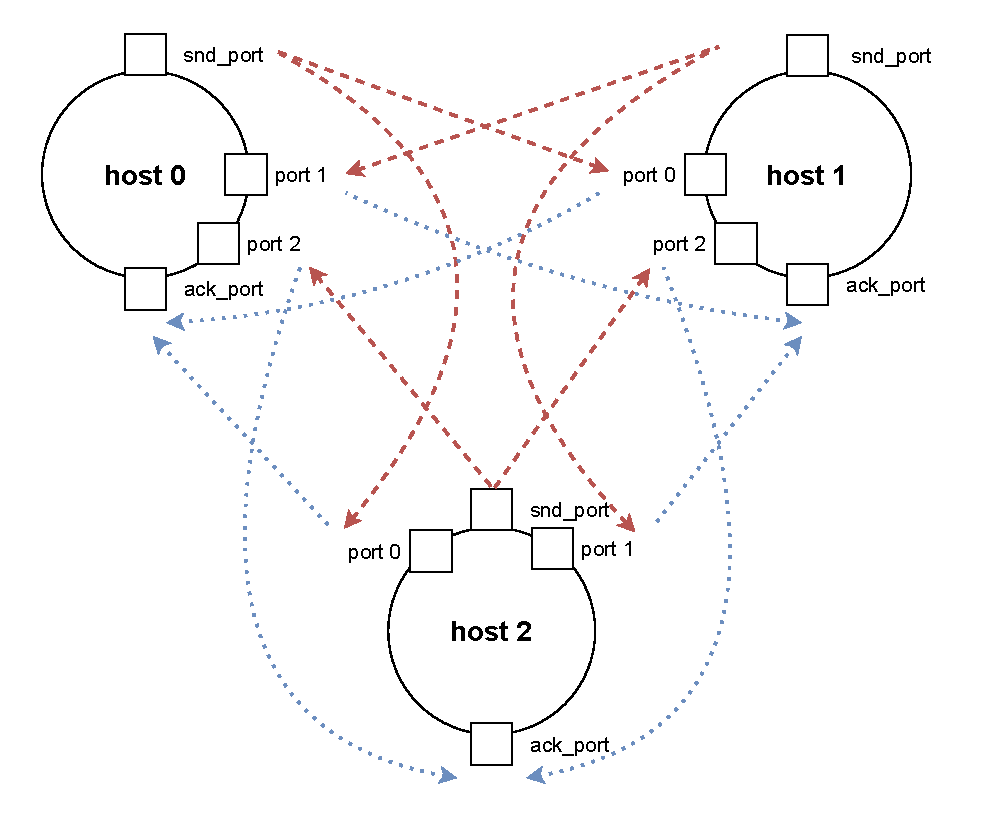
\includegraphics[width=1.0\textwidth]{Img/comm_port.drawio.pdf}
                  \bicaption{端口算法设计示例图}{Example diagram of the port algorithm design}
                  \label{fig:mjiajia-port-design}
              \end{figure}

              \begin{figure}[H]
                  \centering
                  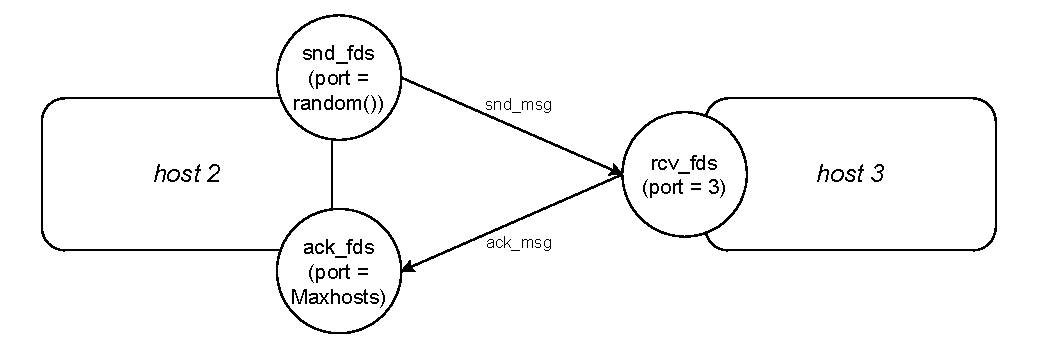
\includegraphics[width=1.0\textwidth]{Img/udp_comm_process.drawio.pdf}
                  \bicaption{UDP单次通信实例}{Example of UDP communication process}
                  \label{fig:mjiajia-comm}
              \end{figure}

        \item \textbf{多线程架构设计}

              在JIAJIA的设计中,使用了SIGIO信号和select组合的多路复用,不过这种方案存在以下不足:
              \begin{itemize}
                  \item SIGIO信号可能在程序执行的任何时刻被触发,需要确保信号处理程序的逻辑是可重入且线程安全的。这涉及到在临界区域处理和返回确认消息时屏蔽信号。
                  \item SIGIO信号是非排队信号,多个 I/O 事件触发信号而信号在处理中被阻塞,后续信号可能丢失。
                  \item 每次信号触发都需要从内核态切换到用户态执行处理函数,频繁的信号涉及大量上下文切换开销。
              \end{itemize}

              为了克服上述缺陷,M-JIAJIA 采用图~\ref{fig:mjiajia-multithread}所示的多线程架构设计。
              该架构将通信任务划分为发送、接收和处理三个子任务,并为每个子任务分配独立线程执行,以提高并发效率。
              \begin{figure}[H]
                  \centering
                  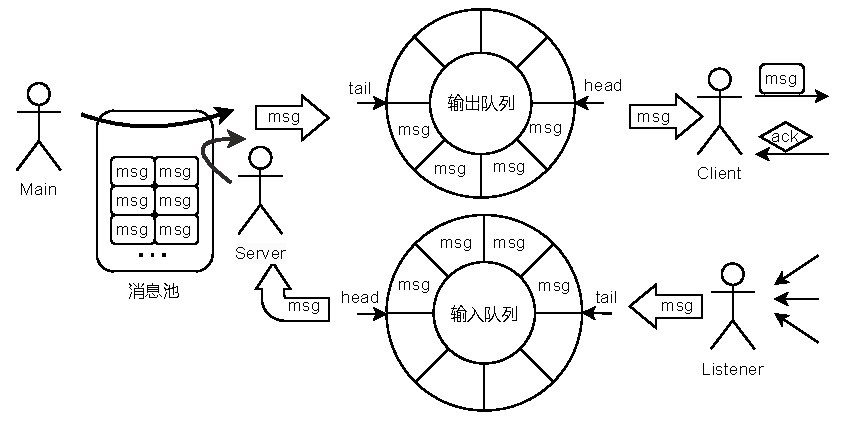
\includegraphics[width=1.0\textwidth]{Img/多线程架构设计.drawio.pdf}
                  \bicaption{\enspace 多线程架构设计}{\enspace Multithread architecture design}
                  \label{fig:mjiajia-multithread}
              \end{figure}

              架构的数据通道依赖于消息池和循环消息队列两个关键数据结构,核心逻辑由发送线程(client)、侦听线程(listener)和服务线程(server)实现。

              \textbf{消息池}:M-JIAJIA在消息池中包含大量预先分配的消息对象,发送消息的线程可以直接从消息池中拿到空闲对象使用,避免频繁分配空间的开销。
              这种设计采用以空间换时间的策略,在高吞吐场景下可以大大提高消息组装的效率;

              \textbf{循环消息队列}:循环消息队列是 M-JIAJIA 核心模块层和通信层之间的通信渠道。
              UDP 通信栈包含输入队列(inqueue)和输出队列(outqueue)两个循环消息队列,分别用于存放接收到的消息和待发送的消息;

              \textbf{发送线程}: 发送线程主要负责检测输出队列是否有待发送的消息,并监听Ack确定消息发送是否成功或需要重传。伪代码如算法~\ref{alg:client-thread} 所示:

              \begin{algorithm}[H]
                  \caption{client thread algorithm}\label{alg:client-thread}
                  \begin{algorithmic}[1] % [1] 使得每行都有行号
                      \Procedure{ClientThread}{}
                      \State initialize $epollfd \gets$ \Call{epoll\_create}{$1$}
                      \State add $epollfd \gets ack\_fds$
                      \While{$true$}
                      \State \Call{sem\_wait}{$outqueue.busy\_count$}
                      \State $msg\_ptr \gets$ \Call{dequeue}{$outqueue$}
                      \For{$retries\_num \gets 0$ to RETRYNUM}
                      \If{$!$ \Call{outsend}{$msg\_ptr$}}
                      \State $break$
                      \EndIf
                      \EndFor
                      \State $snd\_seq[msg\_ptr$->$topid]$++
                      \State \Call{sem\_post}{$outqueue.free\_count$}
                      \EndWhile
                      \State \textbf{return}
                      \EndProcedure

                      \Function{outsend}{$msg$}
                      \If{$msg$->$topid$ = $msg$->$frompid$}
                      \State \textbf{return} \Call{enqueue}{$inqueue,msg$}
                      \Else
                      \State initialize $to\_addr \gets \{msg$->$topid.ip,snd\_port \}$
                      \State \Call{sendto}{$snd\_fds,to\_addr,msg$}
                      \EndIf

                      \While{$true$}
                      \State $nfds \gets$ \Call{epoll\_wait}{$epollfd$}
                      \State \Call{recvfrom}{$ackfds,ack$}
                      \State \textbf{assert}~$\{ack.sid = msg$->$topid\}\;$
                      \State \textbf{assert}~$\{ack.seqno = msg$->$seqno+1\}\;$
                      \State $break$
                      \EndWhile
                      \State \textbf{return} $0$
                      \EndFunction
                  \end{algorithmic}
              \end{algorithm}

              \textbf{侦听线程}:侦听线程负责监视多个接收文件描述符,从就绪的文件描述符中接收消息,将其放入队列,并返回确认消息(Ack)。伪代码如算法~\ref{alg:listen-thread}所示。

              \begin{algorithm}[H]
                  \caption{listen thread algorithm}\label{alg:listen-thread}
                  \begin{algorithmic}[1] % [1] 使得每行都有行号
                      \Procedure{ListenThread}{}
                      \State initialize $epollfd \gets$ \Call{epoll\_create}{$Maxhosts$}
                      \For{$i \gets 0$ to Maxhosts}
                      \State add $epollfd \gets rcv\_fds[i]$
                      \EndFor
                      \While{$true$}
                      \State $nfds \gets$ \Call{epoll\_wait}{$epollfd,events,Maxhosts$}
                      \For{$i \gets 0$ to $nfds$}
                      \State $sockfd \gets events[i].data.fd$
                      \State \Call{recv\_from}{$sockfd,msg$}

                      \State
                      \State $ack \gets \{ msg.seqno+1, msg.topid \}$
                      \State initialize $ack\_addr \gets \{ ack\_port,hosts[msg.frompid].ip \}$
                      \State \Call{sendto}{$sock\_fd,ack\_addr,ack$}

                      \State
                      \If{!\textbf{assert}~$\{msg.seqno = rcv\_seq[to\_id]\}\;$}
                      \State $rcv\_seq[to\_id]$++
                      \State \Call{enqueue}{$inqueue,msg$}
                      \EndIf
                      \EndFor
                      \EndWhile
                      \State \textbf{return}
                      \EndProcedure
                  \end{algorithmic}
              \end{algorithm}

              \textbf{服务线程}:服务线程负责从输入队列中提取消息,并根据消息类型进行相应的服务。伪代码如算法~\ref{alg:server-thread} 所示。
              \begin{algorithm}[H]
                  \caption{server thread algorithm}\label{alg:server-thread}
                  \begin{algorithmic}[1] % [1] 使得每行都有行号
                      \Procedure{ServerThread}{}
                      \State \Call{sem\_wait}{$inqueue.busy\_count$}

                      \State $msg\_ptr \gets$ \Call{dequeue}{$inqueue$}
                      \State \Call{msg\_handle}{$msg\_ptr$}

                      \State \Call{sem\_post}{$inqueue.free\_count$}
                      \State \textbf{return}
                      \EndProcedure
                  \end{algorithmic}
              \end{algorithm}

        \item \textbf{可靠通信实现}

              针对 UDP 协议无连接、不可靠的传输特性,M-JIAJIA 系统在应用层采用消息序号、确认与超时重传机制实现可靠通信,见图~\ref{fig:mjiajia-reliable-comm}。

              \textbf{消息序号}:消息序号用于确保通信的有序性。通信管理器维护与每个远端节点通信的当前消息序号,发送线程从输出队列中获取消息后,将据此为消息分配序号。

              \textbf{确认消息}:每当接收到一条消息,侦听线程会生成并返回相应的确认消息(Ack)。Ack由两部分组成:期望接收的下一个消息的序号以及本机标识。

              \textbf{超时重传机制}:发送线程在发送消息后进入阻塞状态,等待 Ack 消息。如果超时未收到 Ack,则触发重传机制。然而,对于不匹配的 Ack,系统仅忽略处理,不触发重传。
              \begin{figure}[H]
                  \centering
                  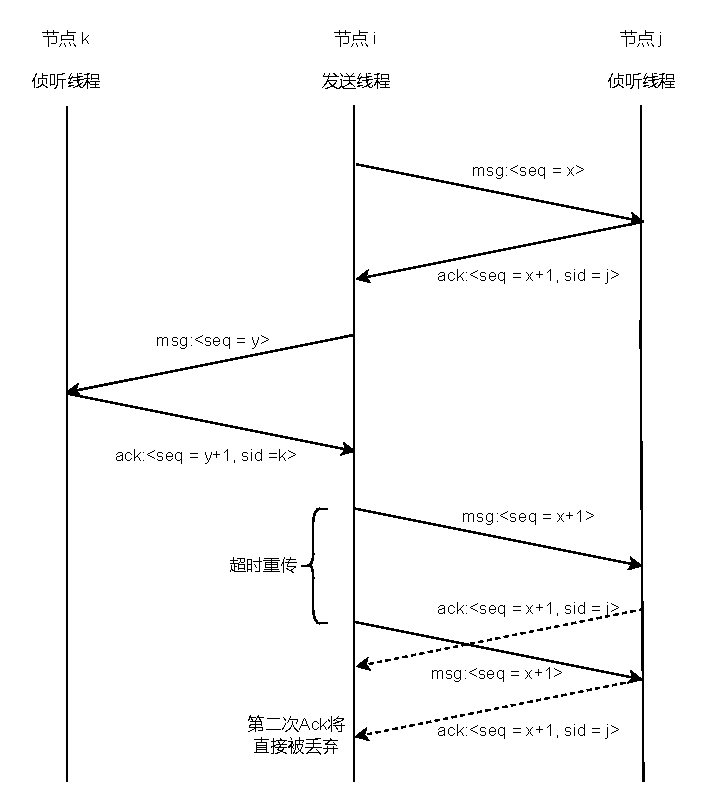
\includegraphics[width=1\textwidth]{Img/M-JIAJIA 可靠通信实现.drawio.pdf}
                  \bicaption{\enspace M-JIAJIA 可靠通信实现}{\enspace M-JIAJIA Reliable Communication Implementation}
                  \label{fig:mjiajia-reliable-comm}
              \end{figure}

    \end{enumerate}

    \subsubsection{RDMA 通信栈设计}
    RDMA 通信模块包含 RDMA 通信栈的设计与实现,这部分将在第~\ref{chap:RJIAJIA}章节介绍。

    \subsection{远程预取优化}
    对于软件 DSM 系统而言,远程内存访问开销是通信开销的重要组成部分,也是影响系统性能的关键因素之一。
    尽管 RDMA 高速网络显著降低了通信延迟,但远程内存访问的开销仍比本地内存访问高 1 至 2 个数量级~\citep{cai2018gam}。
    为此,远程预取技术被广泛研究和应用,以优化数据访问模式,减少远程访问延迟,从而提升系统整体性能。

    M-JIAJIA 的缓存策略是将远端页缓存至本机相同的虚拟地址空间,即共享地址为 addr 的远端页将在本机的 addr 虚拟地址上进行缓存。

    M-JIAJIA 的预取策略是在远程取页时,提前获取远端节点上分配的后续几页共享页,缓存至本地并赋予读权限,从而提升访问效率。

    具体实现方案依赖于三个变量:预取开关(prefetch)、预取页数(prefetch\_pages)和最大检查页数(max\_checking\_pages)。预取的触发条件是:
    $$
        \left\{
        \begin{aligned}
             & \texttt{prefetch = on},           \\
             & \texttt{prefetch\_pages > 0},     \\
             & \texttt{max\_checking\_pages > 0}
        \end{aligned}
        \right.
    $$

    在启用预取的情况下,远端节点在接收到读取页请求后,将最多向后检查 max\_checking\_pages 相邻页是否是共享页,并至多打包 prefetch\_pages 页一同返回。预取优化的效果取决于两次消息传递获取写权限的模式出现的概率以及共享内存的分配策略。若采用循环页分配算法,使相邻页分配至不同节点,预取优化的效果将受到限制。


    \subsection{其他优化}
    \begin{itemize}
        \item M-JIAJIA 优化了 .jiahosts 的处理逻辑,仅依赖 IP 地址、用户名和密码三元组,无需依赖系统配置文件 /etc/hosts;
        \item M-JIAJIA 引入了 .jiaconf 配置文件,以支持自定义系统通信环境和资源管理;
        \item M-JIAJIA 引入了分级日志机制,以满足不同详细程度的调试需求。
    \end{itemize}

    \section{本章小结}
    本章 3.1 节给出 M-JIAJIA 系统的整体框架图,简要介绍了其基本层次结构。

    本章 3.2 节主要介绍 M-JIAJIA 的函数接口。包括配置文件,系统的基本操作和使用说明。

    本章 3.3 节介绍了 M-JIAJIA 的核心模块设计,相比JIAJIA增加了一个RDMA通信模块。

    本章 3.4 节介绍了 M-JIAJIA 相比JIAJIA的一些优化,包括通信栈优化,远程预取优化等。
}

\chapter{RDMA 通信栈的设计与实现}\label{chap:RJIAJIA}{
    本章主要介绍 M-JIAJIA系统中 RDMA 通信栈的架构设计与实现方案。作为通信层组件,RDMA 通信栈与 UDP 通信栈均可用于完成系统消息通信任务,用户可根据底层通信环境在系统运行前通过 .jiaconf 配置实现通信栈的动态切换。在架构设计上,RDMA 和 UDP 通信栈均采用多线程设计,但由于 RDMA通信栈与底层网络适配器深度集成,在实现上与 UDP 通信栈呈现显著差异。

    RDMA 通信首先需要根据应用场景选择合适的通信模式和通信原语,并基于所选模式和原语构建 RDMA 通信管理器,以管理所需的通信资源。随后,根据通信链路模式执行建连后通信或无连接通信。

    \section{设计概览}

    \subsection{RDMA 通信模式与通信原语选择}
    RDMA 支持四种通信模式:可靠连接(RC)、不可靠连接(UC)、可靠数据报(RD)、不可靠数据包(UD)。通信模式不仅决定数据传输的可靠性、有序性和连接方式,还影响通信原语的选择。不同的通信模式适用于不同的应用场景。

    \textbf{RC 模式}: RC 模式采用面向连接的方式,提供可靠且有序的传输服务。通信开始前,需要在通信双方的RC QPs之间建立私有连接。连接建立后,双方将以消息为基本单元进行通信。

    RC 模式具有可靠且有序的传输特性,且支持单向 Verbs 和原子操作,使其被广泛应用在对数据一致性、完整性和顺序性要求较高的场景中。例如,分布式存储系统 ~\citep{christopher2013pilaf, drago2014farm, xingda2020xstore}、高性能计算 ~\citep{graham2005OpenMPI, Huang2006MVAPICH2} 以及分布式事务系统 ~\citep{xingda2018DrTM+H} 等领域。

    \textbf{UC 模式}:UC 模式可视为 RC 模式的子集,面向连接但提供不可靠的传输服务(即不提供 Ack/Nak响应机制,不保证消息被对端成功接收),
    适用于对可靠性要求较低但对性能要求较高的场景,例如某些对实时性要求较高的视频应用。
    此外,在具备强大容错机制的分布式系统中 ~\citep{kalia2014herd},UC 模式相比于 RC 模式可减少网络间通信流量,提升数据传输效率。

    \textbf{RD 模式}:目前尚未有硬件支持 RD 模式,因此该模式尚未在实际应用中得到推广。

    \textbf{UD 模式}:UD 模式提供不可靠的数据报服务,无需建立连接,单个 QP 即可通过单播、多播或广播与其他 UD QPs 进行通信,但最大消息大小受 MTU 限制,适用于对可靠性要求较低或在应用层实现可靠性、规模较大且需要多播的应用场景~\citep{kalia2014herd,kalia2016fasst}。

    M-JIAJIA 在可靠连接(RC)模式下采用 Send 原语进行消息传递,这一设计选择主要基于考虑
    M-JIAJIA 对通信可靠性要求严格,而 RC 模式不仅免除了应用层的分片处理,还省去了额外的可靠性与有序性保障,从而大大简化了系统设计。

    图~\ref{fig:mjiajia-send-recv}显示了 RC 模式下使用 Send 原语发送固定大小消息的示例,图中省略了队列对之间的私有连接以及完成队列元素的生成与处理。为了实现图示通信,M-JIAJIA 采用 RDMA CM 完成建连操作。而且考虑到发送与接收的差异,M-JIAJIA 使用公共输出队列与连接私有输入队列的方案来降低消息队列空间占用。此外,M-JIAJIA 应用多线程优化通信架构设计,以提升整体性能。
    \begin{figure}[H]
        \centering
        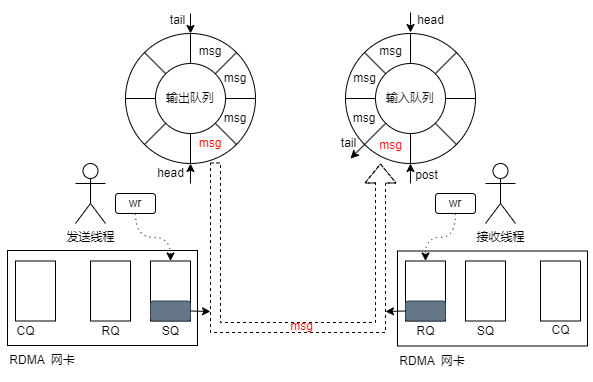
\includegraphics[width=\textwidth]{Img/RDMA-send-receive.png}
        \bicaption{\enspace RDMA 通信栈可靠连接 Send 示例}{\enspace RDMA communication stack reliable connection Send example}
        \label{fig:mjiajia-send-recv}
    \end{figure}



    \subsection{RDMA 通信管理器设计}

    M-JIAJIA 的 RDMA 通信管理器(jia\_context\_t)旨在管理 RDMA 通信所涉及的资源和配置参数。具体可分为以下几部分:

    \begin{enumerate}[label=\arabic*., leftmargin=1em, align=left]
        \item \textbf{RDMA 设备相关信息}
              \begin{itemize}
                  \item \textbf{设备上下文}:设备上下文是应用程序与 RDMA 硬件之间的接口,用于管理所有其他 RDMA 资源。
                  \item \textbf{设备端口号}:设备端口号用于标识 RDMA 设备进行通信的物理端口。
              \end{itemize}

        \item \textbf{RDMA 资源管理信息}
              \begin{itemize}
                  \item \textbf{保护域}:保护域(Protect Domain, PD)是一种资源隔离手段,在RC 模式下用于限制 QPs 可以访问内存区域(Memory Region,MR)的范围。
                  \item \textbf{内存区域}:内存区域是应用程序注册后可被 RDMA 设备直接访问的内存。M-JIAJIA 采用 Send 原语进行通信,因此需分别为发送和接收准备独立的内存区域。在多通信场景下,考虑到输入的不确定性,M-JIAJIA 采用单输出、多输入的内存区域设计方案。
              \end{itemize}

        \item \textbf{RDMA 事件通知信息}
              \begin{itemize}
                  \item \textbf{完成事件通道}:完成事件通道提供 CQ 事件通知机制,用于通知工作请求是否完成。M-JIAJIA 提供独立的发送和接收完成事件通道。
              \end{itemize}

        \item \textbf{RDMA 连接管理信息}
              \begin{itemize}
                  \item \textbf{RDMA 连接管理结构}:该结构用于管理与每个连接相关的信息。包括连接状态、发送序号和接收序号、RDMA 连接管理标识符(rdma\_cm\_id)、输入队列和输入内存区域。
                  \item \textbf{RDMA 连接管理结构数组}:连接管理结构数组记录了与每个远端节点的连接信息。
                  \item \textbf{RDMA 建立连接线程标识}:M-JIAJIA 采用客户端-服务器模式建立连接。在建连阶段,节点分别创建客户端和服务器线程以完成连接。其建连方案具有独特性:每个节点至多创建一个服务器线程用于监听连接请求,同时可创建多个客户端线程主动发起连接。线程标识用于存储和管理线程的信息,便于线程创建、同步和管理。
              \end{itemize}

        \item \textbf{配置参数}
              \begin{itemize}[leftmargin=*, nosep]
                  \item \textbf{批处理数目}: 该参数在 M-JIAJIA 中用于指定在下发接收工作请求时一次下发的工作请求的数量
              \end{itemize}
    \end{enumerate}

    % \begin{lstlisting}[style=CStyle]
    % typedef struct jia_context {
    %     struct ibv_context *context;
    %     struct ibv_pd *pd;                      // common pd
    %     struct ibv_comp_channel *recv_comp_channel;  // common recv io completion channel
    %     struct ibv_comp_channel *send_comp_channel;

    %     // port related
    %     int ib_port;                   // ib port number

    %     // info data
    %     int batching_num; // post recv wr doorbell batching num

    %     // rdma connect (Maxhosts inqueues, only one outqueue)
    %     msg_queue_t *outqueue;
    %     struct ibv_mr *out_mr[QueueSize];
    %     rdma_connect_t connect_array[Maxhosts];

    %     // connection parameters
    %     pthread_t server_thread;   // server thread for connection from client on other hosts
    %     pthread_t *client_threads; // client threads used to connect other hosts
    % } jia_context_t;

    % typedef struct rdma_connect {
    %     bool connected;
    %     unsigned    snd_seq;
    %     unsigned    rcv_seq;
    %     struct rdma_cm_id id;

    %     struct ibv_mr **in_mr;
    %     msg_queue_t *inqueue;
    % } rdma_connect_t;
    % \end{lstlisting}

    \subsection{RDMA 通信栈组成模块}

    为构建基于 RDMA 可靠连接(RC)的通信系统,RDMA 通信栈的初始化流程分为以下四个主要阶段(如图~\ref{fig:mjiajia-rdma-modules}右侧所示):
    \begin{enumerate}[label=\arabic*.]
        \item 初始化上下文。包括获取设备列表、选择硬件设备、打开设备获取上下文、配置物理端口以及输入/输出消息队列初始化等步骤。
        \item 建立连接。通过创建线程向其他主机发起建连请求、并响应其他主机的连接请求,完成任意两节点之间的建连。
        \item 初始化通信资源。主要用于注册输入/输出内存区域(MR)。
        \item 多线程通信。创建线程分别负责下发发送/接收工作请求(WR),同时创建专门处理消息的线程,以优化通信效率。
    \end{enumerate}

    \begin{figure}[!htbp]
        \centering
        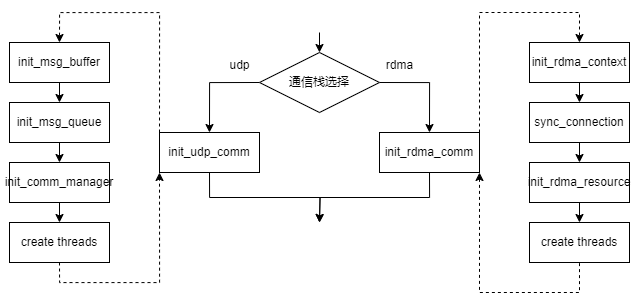
\includegraphics[width=\textwidth]{Img/RDMA-comm-modules.png}
        \bicaption{\enspace M-JIAJIA 通信栈}{\enspace M-JIAJIA communication stack}
        \label{fig:mjiajia-rdma-modules}
    \end{figure}

    \section{可靠通信连接建立机制}
    M-JIAJIA 采用基于 RDMA CM 的建连方式。该方式具有三个显著优势:
    \begin{enumerate}[label=\arabic*.]
        \item 编程简单,RDMA CM 封装了底层复杂的连接建立过程,(使开发者无需直接操作Verbs API即可完成通信流程。
        \item 开销低,RDMA CM 支持异步操作模式,通过事件通道(Event Channel)实现非阻塞通信,避免轮询带来的开销。
        \item 可移植性强,RDMA CM 兼容InfiniBand、RoCEV2和iWARP多种 RDMA 实现,无需针对不同硬件进行代码修改。
    \end{enumerate}

    如图~\ref{fig:mjiajia-cm-connection}所示,建连过程需要客户端和服务器紧密配合,共同完成一系列复杂的步骤,最终生成用于通信的 rdma\_cm\_id 。

    \begin{figure}[H]
        \centering
        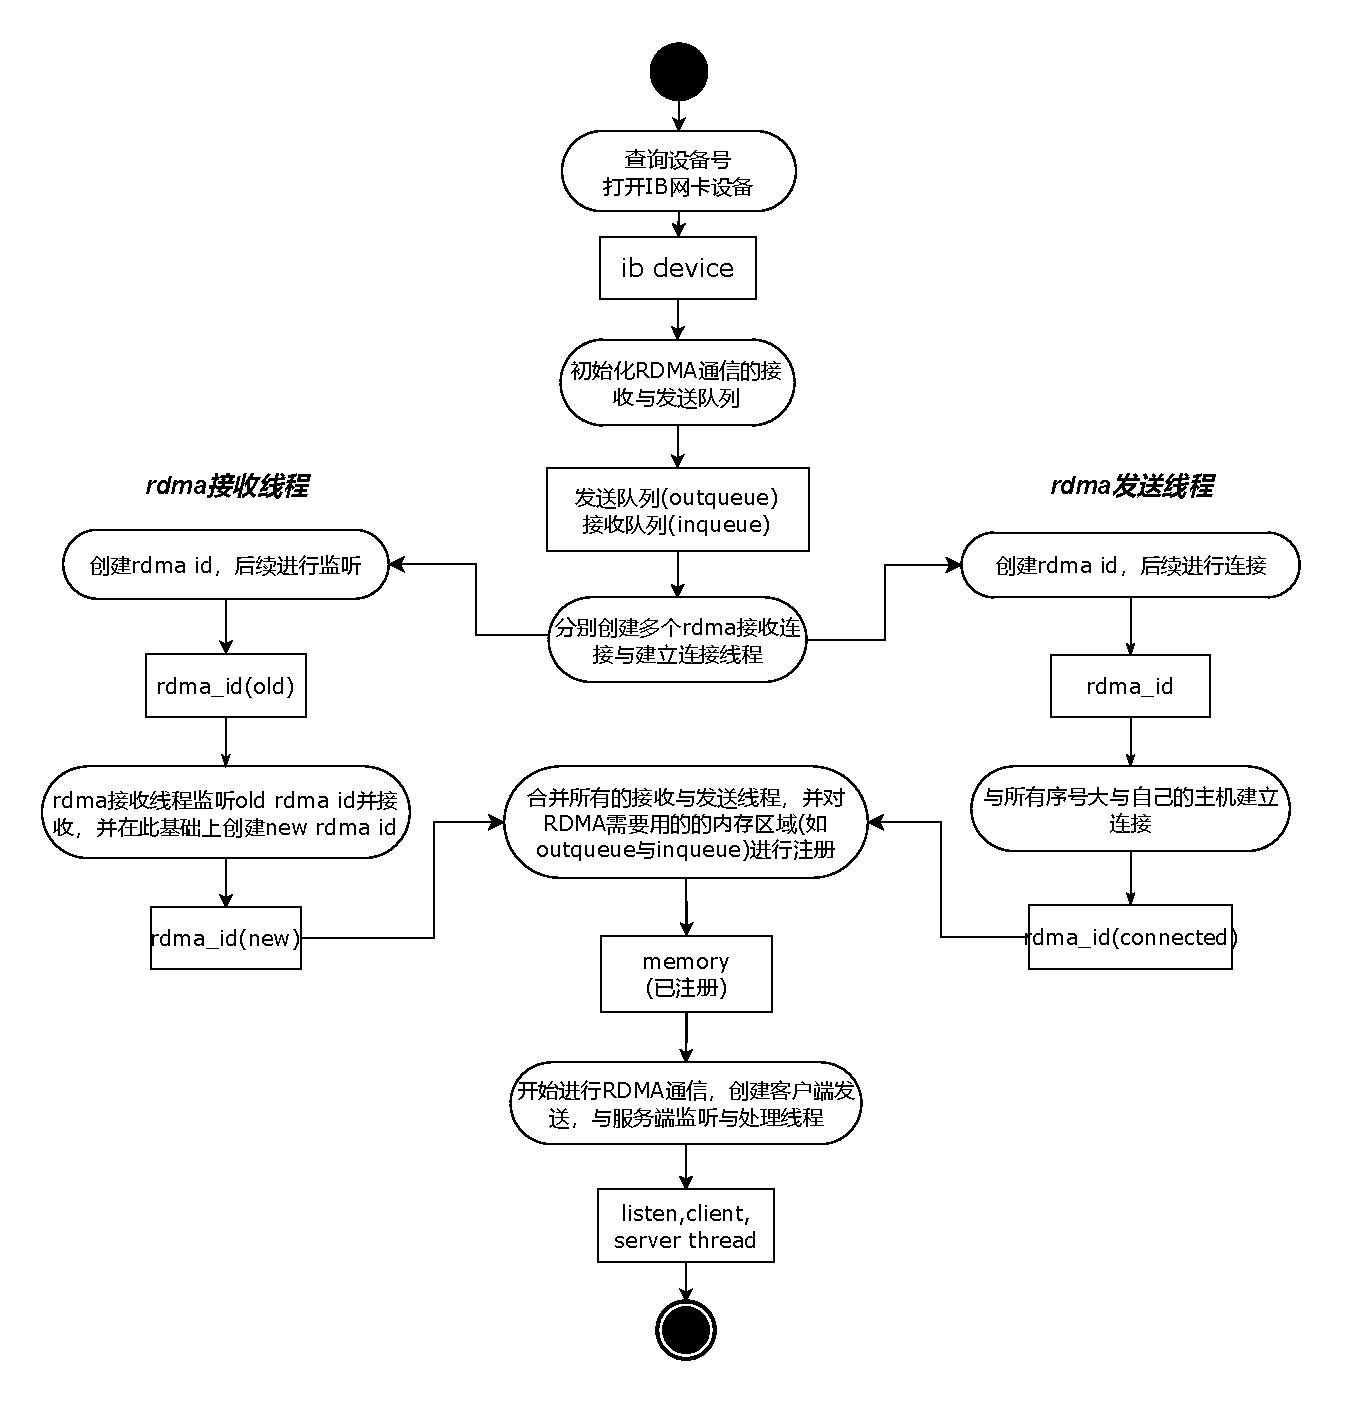
\includegraphics[width=\textwidth]{Img/rdma_init.drawio.pdf}
        \bicaption{M-JIAJIA RDMA CM 建连流程图}{M-JIAJIA RDMA CM Connection Establishment Flowchart}
        \label{fig:mjiajia-cm-connection}
    \end{figure}

    \subsection{建连客户端与服务器}

    % \begin{algorithm}
    %     \caption{RDMA Client Connection Thread}
    %     \begin{algorithmic}[1]
    %         \Procedure{SyncClientThread}{arg}
    %             \State $server\_id \gets$ \Call{ConvertToInt}{arg}
    %             \State $retry\_flag \gets true$, $retry\_count \gets 0$

    %             \State $ec \gets$ \Call{RdmaCreateEventChannel}{}

    %             \While{$retry\_flag$ \textbf{and} $retry\_count < MAX\_RETRY$}
    %                 \State $retry\_flag \gets false$
    %                 \State $id \gets$ \Call{RdmaCreateId}{$ec$}
    %                 \State $addr \gets$ \Call{SetAddress}{$server\_id$}
    %                 \State \Call{RdmaResolveAddr}{$id$, $addr$, $2000$}

    %                 \State
    %                 \While{true}
    %                     \State \Call{RdmaGetCmEvent}{$ec$, $event$}

    %                     \If{$event.type = RDMA\_ROUTE\_RESOLVED$}
    %                         \State $client\_id \gets event.param.conn.private\_data$
    %                         \State $ctx.recv\_comp\_channel \gets$ \Call{CreateCompletionChannel}{}
    %                         \State $ctx.send\_comp\_channel \gets$ \Call{CreateCompletionChannel}{}

    %                         \State
    %                         \State Initialize $qp\_attr$
    %                         \State Request CQ notifications
    %                         \State $ctx.pd \gets$ \Call{Allocate}{$event.id$}
    %                         \State \Call{CreateQP}{$event.id$, $ctx.pd$, $qp\_attr$}

    %                         \State
    %                         \State Initialize $conn\_param$
    %                         \State $event.id \gets$ \Call{RDMAConnect}{$conn\_param$}
    %                     \ElsIf{$event.type = RDMA\_ESTABLISHED$}
    %                         \State Update $ctx.connect\_ array[client\_id]$ connection status
    %                     \Else
    %                         \State \textbf{Default action}
    %                     \EndIf

    %                     \State \Call{RdmaAckCmEvent}{$event$}
    %                 \EndWhile

    %                 \Statex \textbf{NextTry:}
    %             \EndWhile

    %             \Statex \textbf{Cleanup:}
    %             \State \Call{RdmaDestroyEventChannel}{$ec$}
    %             \State \Return NULL
    %         \EndProcedure
    %     \end{algorithmic}
    % \end{algorithm}

    % \begin{algorithm}
    % \caption{RDMA Synchronization Server Thread}
    % \begin{algorithmic}[1]
    %     \State $ec \gets$ \Call{Create\_event\_channel}{$ $} \;
    %     \State $listener \gets$ \Call{Create\_RDMA\_listener\_ID}{$ $} \;
    %     \State Initialize $addr \gets \{ip, start\_port + jia\_pid\}$ \;
    %     \State \Call{Bind\_addr}{$listener, addr$} \;
    %     \While{true}
    %         \State $event \gets$ \Call{rdma\_get\_cm\_event}{$ec$} \;
    %         \If{$event.type = $RDMA\_CM\_EVENT\_CONNECT\_REQUEST}
    %             \State $client\_id \gets event.param.conn.private\_data$ \;
    %             \State $ctx.recv\_comp\_channel,ctx.send\_comp\_channel \gets$ \Call{create\_completion\_channel}{$ $} \;

    %             \State
    %             \State Initialize $qp\_attr$ \;
    %             \State Request CQ notifications \;
    %             \State $ctx.pd \gets$ \Call{allocate}{$event.id$} \;
    %             \State \Call{create\_QP}{$event.id$, $ctx.pd$, $qp\_attr$} \;

    %             \State
    %             \State Initialize $conn\_param$ \;
    %             \State $event.id \gets$ \Call{RDMA\_accept}{$conn\_param$} \;
    %         \ElsIf{$event.type = $RDMA\_CM\_EVENT\_ESTABLISHED}
    %             \State Update $ctx.connect\_array[client\_id]$ connection status \;
    %             \State $completion\_num \gets completion\_num + 1$ \;
    %             \If{$completion\_num = system\_setting.jia\_pid$}
    %                 \State \textbf{goto} Cleanup \;
    %             \EndIf
    %         \Else \quad \textbf{Default action} \;
    %         \EndIf
    %         \State \Call{rdma\_ack\_event}{$event$} \;
    %     \EndWhile

    %     \State
    %     \State \textbf{Cleanup:} \;
    %     \State \Call{Destroy\_RDMA\_listener\_ID}{$listener$} \;
    %     \State \Call{Destroy\_event\_channel}{$ec$} \;
    %     \State \Return \;
    % \end{algorithmic}
    % \end{algorithm}

    \subsection{RDMA 集群建连算法}

    M-JIAJIA 运行时要求任意两节点具备通信能力,因此必须在任意两节点之间至少建立一个连接。
    M-JIAJIA 采用客户端服务器模式,通过创建多个客户线程与服务线程去建立连接,并采用了算法~\ref{alg:connection-algo}所示的建连算法,
    不必为每个连接设立单独的服务器处理。

    \begin{algorithm}
        \caption{RDMA Cluster Connection Establishment Algorithm}\label{alg:connection-algo}
        \begin{algorithmic}[1]
            \Procedure{sync\_connection}{$hosts$, $pid$}
            \If{$pid$ $\neq$ 0}
            \State \Call{pthread\_create}{\&ctx.server\_thread, NULL, server\_thread, \&ctx}
            \EndIf
            \State $num\_clients$ $\gets$ $hosts$ - $pid$ - 1
            \If{$num\_clients$ $>$ 0}
            \State $ctx.client\_threads$ $\gets$ \Call{malloc}{$num\_clients$ * sizeof(pthread\_t)}
            \For{$i \gets 0$ to $num\_clients$}
            \State $target\_hosts$ $\gets$ \Call{malloc}{sizeof(int)}
            \State $*target\_hosts$ $\gets$ $pid + i + 1$
            \State \Call{pthread\_create}{\&ctx.client\_threads[i], NULL, client\_thread, target\_hosts}
            \EndFor
            \EndIf
            \If{$pid$ $\neq$ 0}
            \State \Call{pthread\_join}{ctx.server\_thread, NULL}
            \EndIf

            \If{$num\_clients$ > 0}
            \For{$i \gets 0$ to $num\_clients$}
            \State \Call{pthread\_join}{ctx.client\_threads[i], NULL}
            \EndFor
            \EndIf
            \EndProcedure
        \end{algorithmic}
    \end{algorithm}

    在rdma同步的过程中,主机号偏小的主机会创建多个client线程与主机号偏大的主机server线程尝试建立连接;
    同时除jia\_pid为0外所有的主机都会创建一个server线程来监听建立的rdma连接,最终每两台主机之间建立一个rdma连接;
    如图~\ref{fig:RDMA-connection-build}所示,创建线程并建立连接。



    \begin{figure}[H]
        \centering
        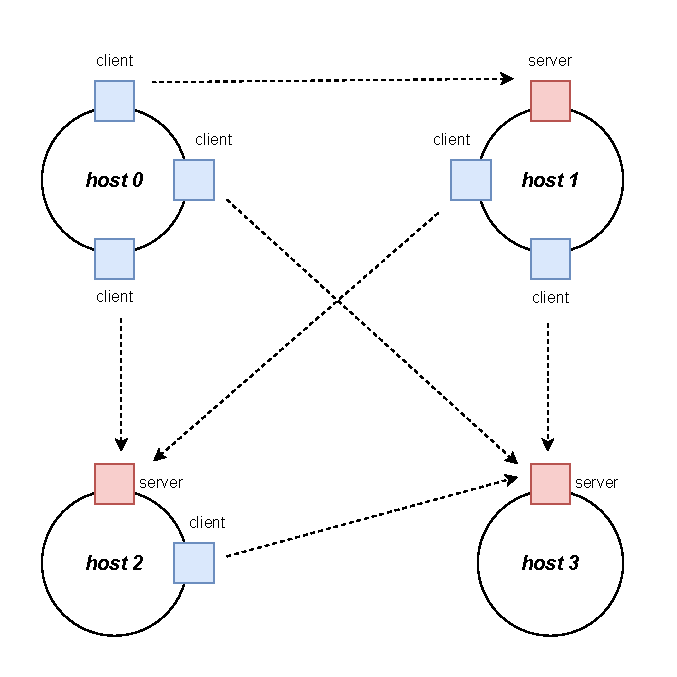
\includegraphics[width=0.65\textwidth]{Img/rdma_sync.drawio.pdf}
        \bicaption{\enspace RDMA集群建连示例}{\enspace RDMA Cluster Connection Establishment Example}
        \label{fig:RDMA-connection-build}
    \end{figure}



    % \begin{figure}[H]
    %     \centering
    % .    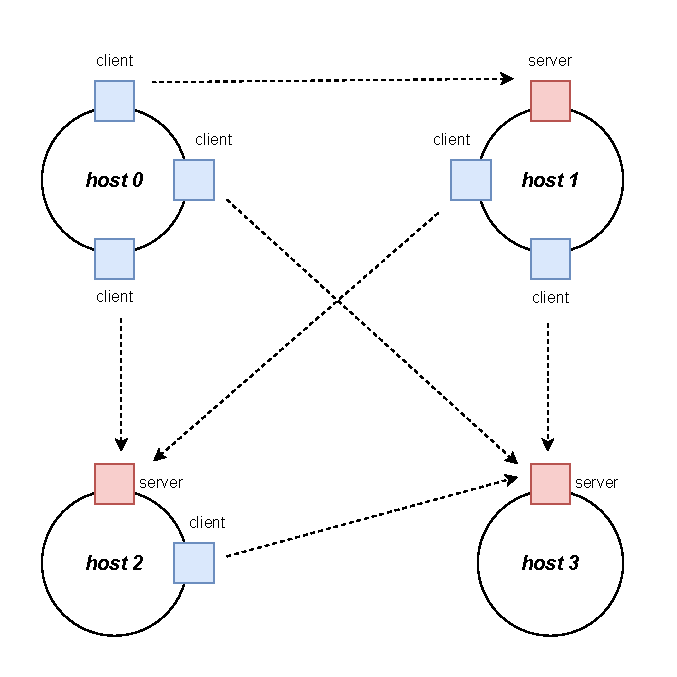
\includegraphics[width=1.0\textwidth]{Img/rdma_sync.drawio.pdf}
    %     \caption{RDMA同步过程中的client与server同步线程}
    % \end{figure}



    \section{RDMA 多线程通信架构设计}

    \begin{figure}[H]
        \centering
        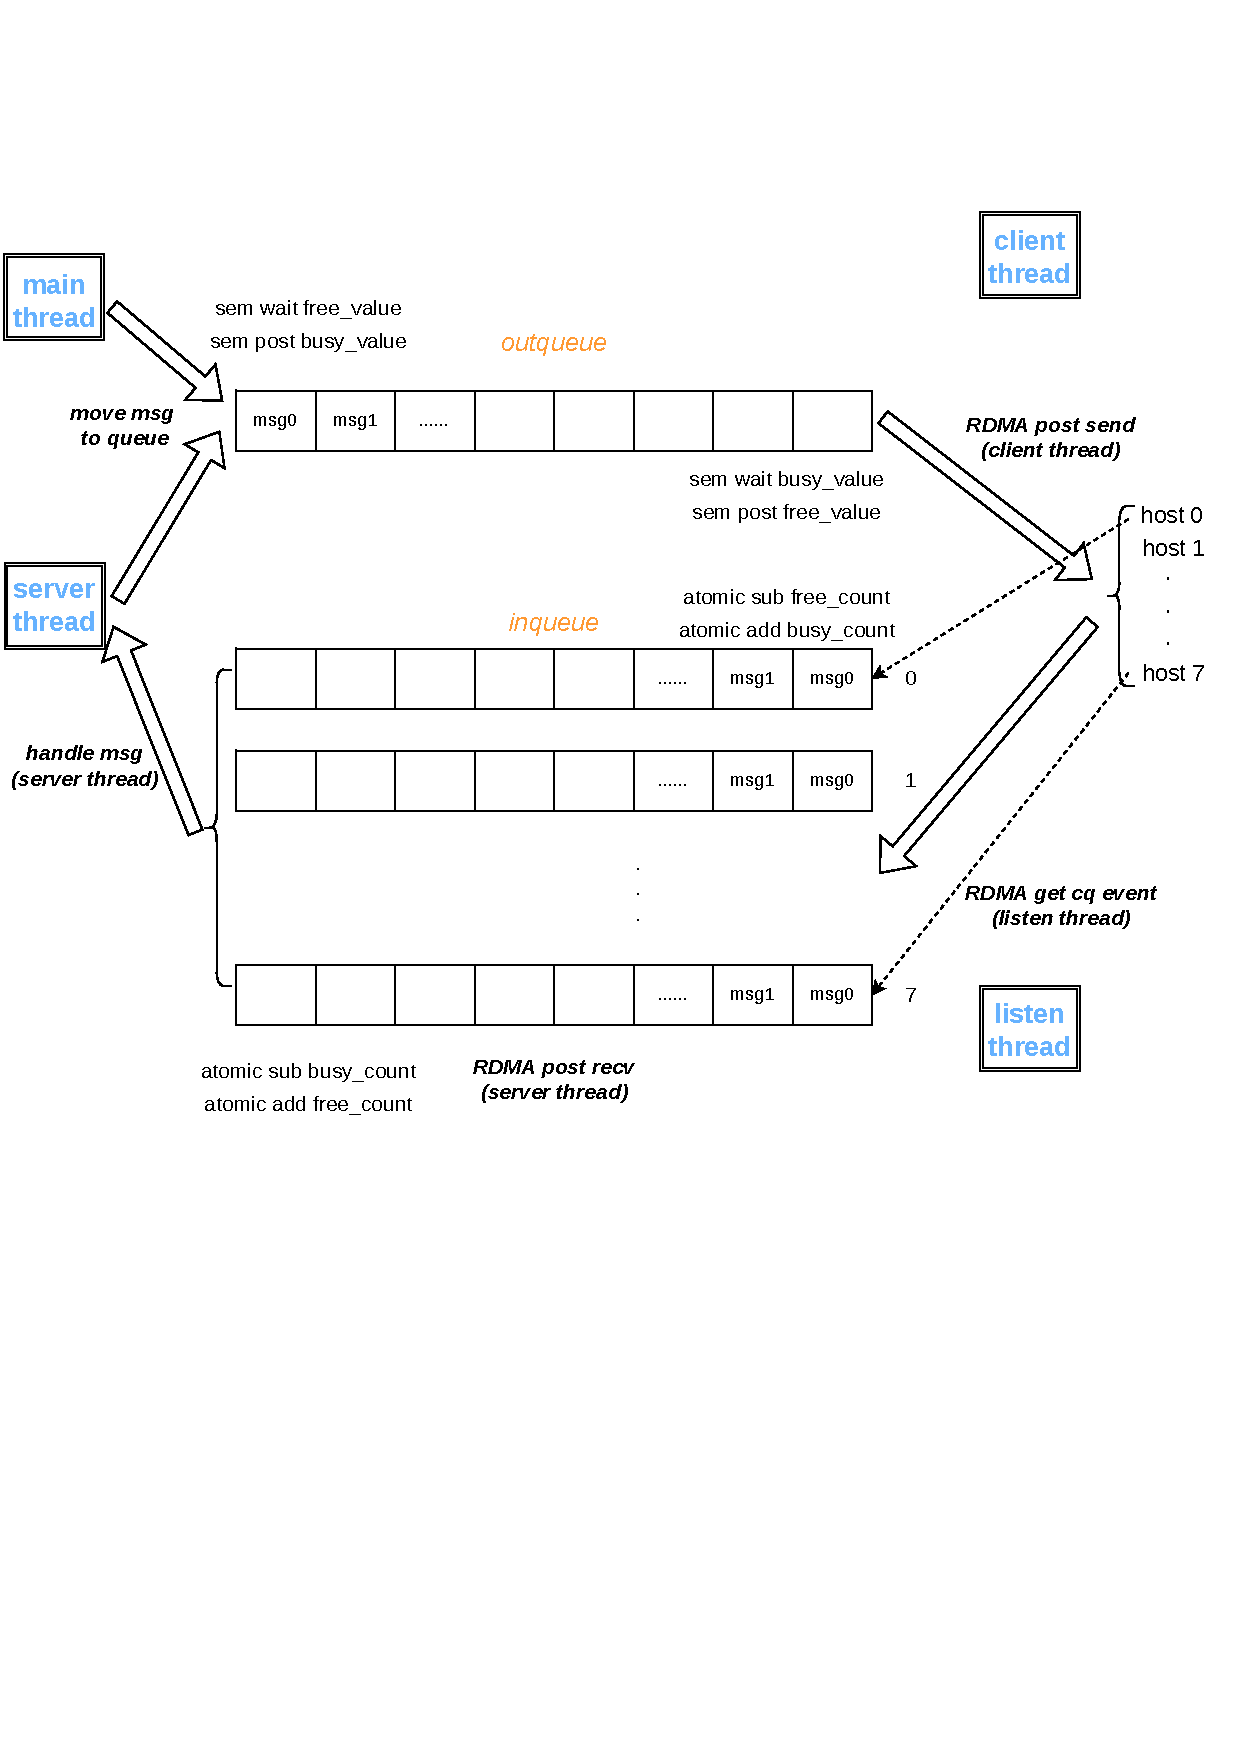
\includegraphics[width=1.1\textwidth]{Img/RDMA_design.pdf}
        \caption{RDMA communication design}
    \end{figure}


    \subsection{RDMA 多线程任务划分}

    \subsubsection{RDMA通信接收端线程任务划分}
    RDMA通信接收端由listen与server两个线程组成,他们的任务划分如下:

    \begin{itemize}[leftmargin=*, nosep]
        \item \textbf{listen thread}:用于监听rdma接收到的msg,并通知server线程进行处理;
        \item \textbf{server thread}:用于处理rdma接收到的msg,同时负责下发任务,即在成功处理完成一个msg后post\_recv该空位,用于下一次接收;
    \end{itemize}

    \begin{figure}[H]
        \centering
        .    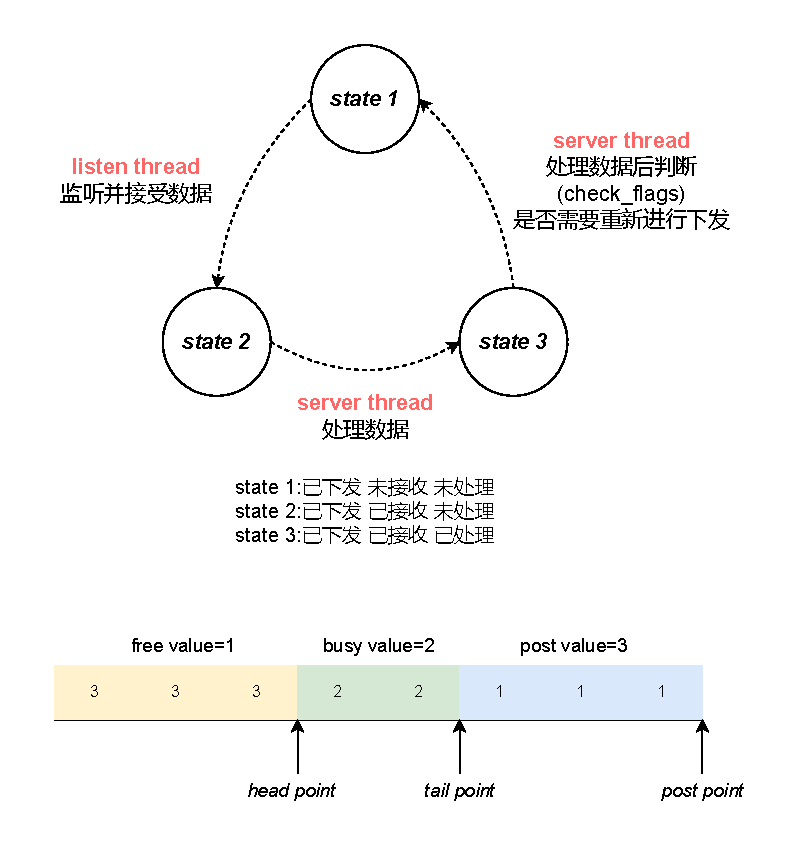
\includegraphics[width=1.0\textwidth]{Img/recv_state.drawio.pdf}
        \caption{RDMA接收端inqueue中msg的状态转换}
    \end{figure}

    listen thread的伪代码如下:
    \begin{algorithm}
        \caption{listen thread algorithm}
        \begin{algorithmic}[1] % [1] 使得每行都有行        
            \Procedure{ListenThread}{}
            \State \Call{post\_recv}{$ $}
            \State \textbf{return} NULL
            \EndProcedure

            \Function{post\_recv}{}
            \While{$true$}
            \State $\{ cq\_ptr, context\} \gets$ \Call{ibv\_get\_cq\_event}{$recv\_comp\_channel$}
            \State $inqueue \gets (rdma\_connect\_t)context.inqueue$
            \State \Call{ibv\_req\_notify\_cq}{$cq\_ptr$}
            \State $wc \gets$ \Call{ibv\_poll\_cq}{$cq\_ptr$}

            \State
            \If{$wc.status \neq \text{IBV\_WC\_SUCCESS}$}
            \State \Call{log\_err}{$post\_recv \quad error$}
            \Else
            \State \Call{atomic\_fetch\_sub}{$inqueue$->$post\_value$}
            \State \Call{atomic\_fetch\_add}{$inqueue$->$busy\_value$}

            \State
            \State $connect\_array[inqueue$->$queue[inqueue$->$tail]$->$topid].rcv\_seq $++
            \State $inqueue$->$tail \gets (inqueue$->$tail$+1$) \% QueueSize$
            \EndIf
            \EndWhile

            \State
            \State \Call{ibv\_ack\_cq\_events}{$cq\_ptr$}
            \State \textbf{return}
            \EndFunction
        \end{algorithmic}
    \end{algorithm}

    \newpage
    server thread的伪代码如下:
    \begin{algorithm}
        \caption{server thread algorithm}
        \begin{algorithmic}[1] % [1] 使得每行都有行号
            \Procedure{ServerThread}{}
            \State \Call{init\_post\_recv\_wr}{$ $}

            \While{$true$}
            \For{$i \gets 0$ to $hostc$}
            \State $tmp\_connect \gets connect\_array[i]$
            \State $in\_queue \gets tmp\_connect$->$inqueue$
            \If{\Call{atomic\_load}{$tmp\_connect.inqueue$->$busy\_value$}}
            \State \Call{msg\_handle}{$inqueue$->$queue[head]$}
            \State \Call{atomic\_fetch\_sub}{$inqueue$->$busy\_value$}
            \State \Call{atomic\_fetch\_add}{$inqueue$->$free\_value$}
            \If{$i == jia\_pid$}
            \State $tmp\_connect.rcv\_seq$ ++
            \EndIf
            \State $inqueue$->$head \gets (inqueue$->$head$+1$) \% QueueSize$
            \EndIf
            \EndFor

            \If{$i \neq jia\_pid$}
            \State \Call{check\_flags}{$i$}
            \EndIf
            \EndWhile
            \State \textbf{return}
            \EndProcedure
        \end{algorithmic}
    \end{algorithm}

    \newpage
    \subsubsection{RDMA通信发送端线程任务划分}
    RDMA通信接收端由main/server两个入队线程,和一个client发送线程组成,他们的任务划分如下:

    \begin{itemize}[leftmargin=*, nosep]
        \item \textbf{main/server thread}:用于下发rdma需要发送的msg,并将msg放入outqueue队列中;
        \item \textbf{client thread}:将对应的msg从outqueue队列中取出,并通过rdma发送msg给对应主机;
    \end{itemize}

    client thread的伪代码如下:
    \begin{algorithm}
        \caption{client thread algorithm}
        \begin{algorithmic}[1] % [1] 使得每行都有行号
            \Procedure{ClientThread}{}
            \While{$true$}
            \State \Call{sem\_wait}{$outqueue.busy\_count$}
            \State $msg\_ptr \gets$ \Call{dequeue}{$outqueue$}
            \State $msg\_ptr$->$seqno \gets connect\_array[msg\_ptr$->$to\_pid]$

            \State
            \If{$msg\_ptr$->$topid$ = $jia\_pid$}
            \State \Call{memcpy}{$inqueue[tail],msg\_ptr$}
            \State \Call{atomic\_fetch\_sub}{$inqueue$->$free\_value$}
            \State \Call{atomic\_fetch\_add}{$inqueue$->$busy\_value$}
            \State $inqueue$->$tail \gets (inqueue$->$tail$+1$) \%QueueSize$
            \Else
            \While{\Call{post\_send}{$connect\_array[msg\_ptr$->$to\_pid]$}}
            \EndWhile
            \EndIf

            \State
            \State $connect\_array[msg\_ptr$->$topid].snd\_seq$++
            \State $inqueue$->$head \gets (inqueue$->$head$+1$) \% QueueSize$
            \State \Call{sem\_post}{$outqueue.free\_count$}
            \EndWhile
            \State \textbf{return}
            \EndProcedure
        \end{algorithmic}
    \end{algorithm}


    \begin{algorithm}
        \caption{client thread post send}
        \begin{algorithmic}[1] % [1] 使得每行都有行号
            \Function{post\_send}{}
            \State initialize $sge \gets \{out\_mr[outqueue$->$head] \}$
            \State initialize $wr \gets \{sge\}$

            \State
            \State $msg\_ptr \gets$ $outqueue[outqueue$->$head]$

            \While{\Call{ibv\_post\_send}{$connect\_array[msg\_ptr$->$pid]$}}
            \EndWhile

            \State
            \State $cq\_ptr \gets$ \Call{ibv\_get\_cq\_event}{$send\_comp\_channel$}
            \State \Call{ibv\_req\_notify\_cq}{$cq\_ptr$}

            \State
            \State $wc \gets$ \Call{ibv\_poll\_cq}{$connect\_array[msg\_ptr$->$topid]$->$send\_cq$}
            \If{$wc.status \neq \text{IBV\_WC\_SUCCESS}$}
            \State \textbf{return} $1$
            \EndIf

            \State
            \State \Call{ibv\_ack\_cq\_events}{$cq\_ptr$}
            \State \textbf{return} $0$
            \EndFunction
        \end{algorithmic}
    \end{algorithm}

    \begin{figure}[H]
        \centering
        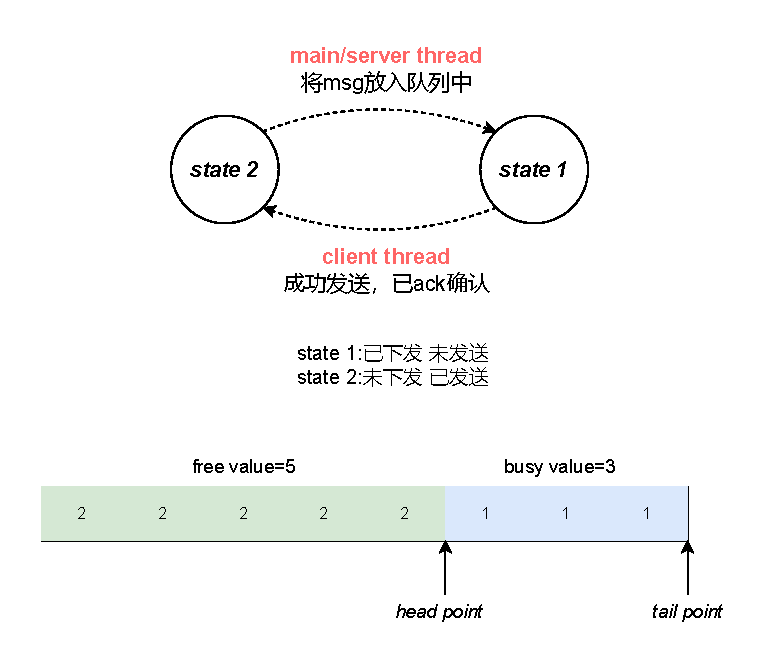
\includegraphics[width=1.0\textwidth]{Img/send_state.drawio.pdf}
        \caption{RDMA发送端outqueue中msg的状态转换}
    \end{figure}


    \newpage
    \subsection{RDMA 多线程通信流程}

    \subsubsection{消息发送流程}
    \begin{enumerate}[leftmargin=1em, align=left]
        \item \textbf{消息入队}:
              \begin{itemize}[leftmargin=*, nosep]
                  \item 应用程序将待发送的消息放入\texttt{outqueue}队列中,队列中的每个消息包含目标主机的IP地址和消息内容。
              \end{itemize}
        \item \textbf{RDMA Send操作}:
              \begin{itemize}[leftmargin=*, nosep]
                  \item 发送端根据消息中的目标主机IP地址,查找对应的RDMA连接上下文(包括QP(Queue Pair)和MR(Memory Region)等信息)。
                  \item 调用\texttt{ibv\_post\_send} API,将消息内容通过RDMA Send操作发送到目标主机。
              \end{itemize}
        \item \textbf{发送完成检测}:
              \begin{itemize}[leftmargin=*, nosep]
                  \item 发送端通过轮询或事件通知机制(如Completion Queue)检测Send操作的完成状态。
                  \item 当检测到Send操作成功完成时,发送端从\texttt{outqueue}队列中移除已发送的消息,并准备发送下一条消息。
              \end{itemize}
        \item \textbf{错误处理}:
              \begin{itemize}[leftmargin=*, nosep]
                  \item 如果Send操作失败,发送端会记录错误日志,并根据配置决定是否重试发送或丢弃该消息。
              \end{itemize}
    \end{enumerate}

    \subsubsection{消息接收流程}
    \begin{enumerate}[leftmargin=1em, align=left]
        \item \textbf{预置Recv Buffer}:
              \begin{itemize}[leftmargin=*, nosep]
                  \item 接收端在初始化时,预先为每个QP下发多个Recv Buffer,通过\texttt{ibv\_post\_recv} API将Recv请求提交到接收队列中。
                  \item 每个Recv Buffer对应一个内存区域,用于存储接收到的消息。
              \end{itemize}
        \item \textbf{消息接收}:
              \begin{itemize}[leftmargin=*, nosep]
                  \item 当发送端发起RDMA Send操作时,接收端的RNIC(RDMA Network Interface Card)会将消息数据直接写入预置的Recv Buffer中。
                  \item 接收端通过轮询或事件通知机制检测Recv操作的完成状态。
              \end{itemize}
        \item \textbf{消息入队}:
              \begin{itemize}[leftmargin=*, nosep]
                  \item 当检测到Recv操作完成时,接收端将接收到的消息从Recv Buffer中取出,并放入\texttt{inqueue}队列中。
                  \item 接收端继续下发新的Recv请求,以确保始终有足够的Recv Buffer接收后续的消息。
              \end{itemize}
        \item \textbf{消息处理}:
              \begin{itemize}[leftmargin=*, nosep]
                  \item 接收端的服务线程(Server Thread)定期轮询\texttt{inqueue}队列,取出消息并进行处理。
                  \item 处理逻辑由应用程序定义,可能包括数据解析、业务逻辑处理、响应生成等。
              \end{itemize}
    \end{enumerate}


    \section{本章小结}本章主要介绍了RDMA通信栈的设计与实现。首先简要介绍RDMA几种常见的通信模式,并探讨了在M-JIAJIA中RDMA的基本通信组成模块和流程;随后介绍了RDMA建连过程中每台主机的client线程与server线程的运作原理;最后探讨了在RDMA通信过程中每台主机相关线程的通信流程。

    本章 4.1 节给出 M-JIAJIA RDMA通信模式与通信原语选择。首先介绍了RDMA基本的几种通信模式(RC,UC,RD,UD模式),并通过画图阐述了M-JIAJIA在RC模式下的通信基本流程;然后探讨了RDMA通信管理器中的相关信息以及通信栈组成模块,并通过画图揭示了RDMA通信的一般流程;

    本章 3.2 节主要介绍 M-JIAJIA 的函数接口。首先,阐述了全局变量 jiahosts 和 jiapid 的作用;随后,详细解析了 jia\_init 初始化模块的执行流程,并介绍 M-JIAJIA 在该模块上的架构优化。接着,探讨了共享内存的分配算法及其对应的接口设计,进一步介绍了消息传递接口和 RMA 接口。最后,以模块概述和使用说明作为小节总结。

    本章 3.3 节介绍了 M-JIAJIA 的核心模块设计,涵盖初始化模块、系统配置模块、内存管理模块、锁管理模块、UDP 通信管理模块、RDMA 通信管理模块及统计模块,并简要阐述其功能与实现机制。

    本章 3.4 节介绍了 M-JIAJIA 的通信层设计,该层包括 UDP 通信栈和 RDMA 通信栈。本节重点探讨 UDP 通信栈的设计,首先阐述 M-JIAJIA 端口占用算法如何将端口占用的复杂度从 $O(n^2)$ 降至 $O(n)$。随后,对比 Linux 系统中的三种多路复用接口——select()、poll() 和 epoll(),并分析 M-JIAJIA 选择 epoll 的原因。接着,介绍 M-JIAJIA 多线程架构设计相较于 JIAJIA 信号驱动 I/O 的优势,并详细说明发送线程、侦听线程和服务线程的实现机制。最后,探讨 M-JIAJIA 如何通过序号、确认及超时重传机制实现可靠通信。

    本章 3.5 节介绍了 M-JIAJIA 的远程预取优化机制,包括共享内存初始化过程中常见的两次消息传递获取写权限模式,以及针对与此 M-JIAJIA 的预取策略。

    本章 3.6 节简要介绍了 M-JIAJIA 在提高系统易用性和可维护性上的工作。包含配置文件和日志机制两部分。
}
\chapter{性能测试与优化分析}\label{chap:experiments}{
    \section{测试程序}\label{sec:测试程序}


    \begin{enumerate}[leftmargin=1em, align=left]
        \item \textbf{WATER}:
              \begin{itemize}[leftmargin=*, nosep]
                  \item Water 是一个用于水分子动力学模拟的程序,它逐步模拟 n 个分子的运动状态。
                        在并行计算中,Water 采用均匀分配策略,将分子数组划分至各个处理机;同时为了减少通信开销,每个处理机维护一个本地备份来存储临时计算得到的作用力;
                        所有处理机计算完毕后,系统才会进入由锁保护的临界区,对全局结果进行更新;这一同步操作由barrier操作来实现;
              \end{itemize}
        \item \textbf{LU}:
              \begin{itemize}[leftmargin=*, nosep]
                  \item LU 采用块分解算法,将稠密矩阵分解为上三角矩阵和下三角矩阵,并使用连续块分配的 LU 分解策略。
                        块 LU 分解算法逐步进行,每次处理一列块。
                        每个步骤包括三个阶段:首先,对对角块进行 LU 分解;然后,将对角块下方的块除以已分解的对角块;
                        最后,更新矩阵右侧的剩余块(trailing blocks)。并行计算主要集中在第三阶段,而每个步骤的三个阶段通过 barrier 操作实现同步;
              \end{itemize}
        \item \textbf{IS}:
              \begin{itemize}[leftmargin=*, nosep]
                  \item IS 是一个基于“桶排序”算法的整数排序程序。
                        它将 key 均匀分配到各个处理机,每个处理机维护一个私有“桶”,同时所有处理机共享一个公用“桶”;
                        对于公用“桶”的共享,将涉及到全局处理机的同步与通信操作;
              \end{itemize}
        \item \textbf{SOR}:
              \begin{itemize}[leftmargin=*, nosep]
                  \item SOR 采用红黑格的逐次超松弛法(Successive Over-Relaxation, SOR)来求解偏微分方程。
                        在并行实现中,红黑两个数组被划分为大小接近的长方块,并分配给不同处理机进行计算,
                        各处理机通过 barrier 操作进行同步,确保所有处理机都能获取最新的计算结果;
              \end{itemize}
        \item \textbf{TSP}:
              \begin{itemize}[leftmargin=*, nosep]
                  \item TSP 采用分支限界算法求解旅行商问题,其核心数据结构包括:
                        用于存储路径的存储池、指向路径的优先队列、存放未使用路径指针的堆栈,以及记录当前最短路径的变量;
                        在搜索最短路径的过程中,算法通过优先队列选择最有希望的路径进行扩展,并在必要时从存储池分配或释放路径。
                        随着搜索的进行,算法不断更新当前最短路径,并利用剪枝策略提高效率;
              \end{itemize}
        \item \textbf{EP}:
              \begin{itemize}[leftmargin=*, nosep]
                  \item EP 的主要目标是生成一组符合高斯分布的数对;
                  \item 该程序具有高度并行性,在整个计算过程中,唯一的通信操作仅发生在最后的累积阶段,用于合并各处理机的计算结果;
              \end{itemize}
        \item \textbf{PI}:

              \begin{itemize}[leftmargin=*, nosep]
                  \item PI 将pi的计算任务切分后分布到不同的主机上,分别计算后最后叠加;
                  \item 该程序具有高度并行性,最后通过对pi这个共享变量的操作将不同主机的计算结果累加;
              \end{itemize}
    \end{enumerate}

    \section{程序开销分析}\label{sec:程序开销分析}
    本小节讨论的程序开销是指从主节点启动程序到所有节点完成任务并返回结果至主节点所耗费的总时间。
    在基于 M-JIAJIA 用户库的并行程序中,主要的开销包括系统初始化开销、计算开销和通信开销。
    下面对以上三种开销分别进行阐述:
    \begin{itemize}
        \item \textbf{系统初始化开销}:

              系统初始化开销代表调用 jia\_init() 初始化 M-JIAJIA 系统所耗费的时间。

              程序分发与远程执行产生的通信开销是系统初始化过程中最主要的性能瓶颈。
              当前,M-JIAJIA采用基于SCP(Secure Copy)的程序分发和SSH(Secure Shell)远程执行机制,
              其单线程串行传输模式导致分发时间随集群规模扩大呈线性增长(如图~\ref{fig:time-create-procs}所示)。
              这种设计并不高效,未来可以通过并行分发策略和采用 RDMA 拷贝协议来降低该部分的开销。

              另一部分系统初始化开销是RDMA通信栈的初始化,这部分的开销如图~\ref{fig:time-init-rdma-comm}所示。
              目前已有研究~\citep{guo2024secm}尝试在建连阶段以流水线方式同时执行多个连接设置以降低该部分的开销。

        \item \textbf{计算开销}:

              计算开销指节点进行任务计算所需的时间。
              计算开销取决于任务规模、划分策略以及硬件性能等因素,但其对通信开销中的同步开销同样有重要影响。

              如图~\ref{fig:ep-performance}所示,基于 M-JIAJIA 的 ep 程序在多节点上执行,ep-i 中的 i 代表参与任务执行的节点数目,
              图中展示了 ep-8 所出现的反常现象,原因是参与并行任务的第八台节点(搭载 AMD EPYC 9754 128核处理器)处理速度过慢,
              导致其他节点在执行 barrier 同步时需要等待将近 17s 的时间(在节点 8 上单独执行 ep 程序需要近 159s 的时间,
              是其他节点单独执行的6-7倍)。因此,合理的计算集群构建方案是采用处理速度相近的节点,或根据处理能力划分任务。

        \item \textbf{通信开销}

              通信开销可以分为两部分,一是因访问远程数据导致的开销,二是维护一致性导致的开销。
              这部分将在 \ref{sec:通信栈} 小节进一步介绍。

    \end{itemize}

    \begin{figure}
        \centering
        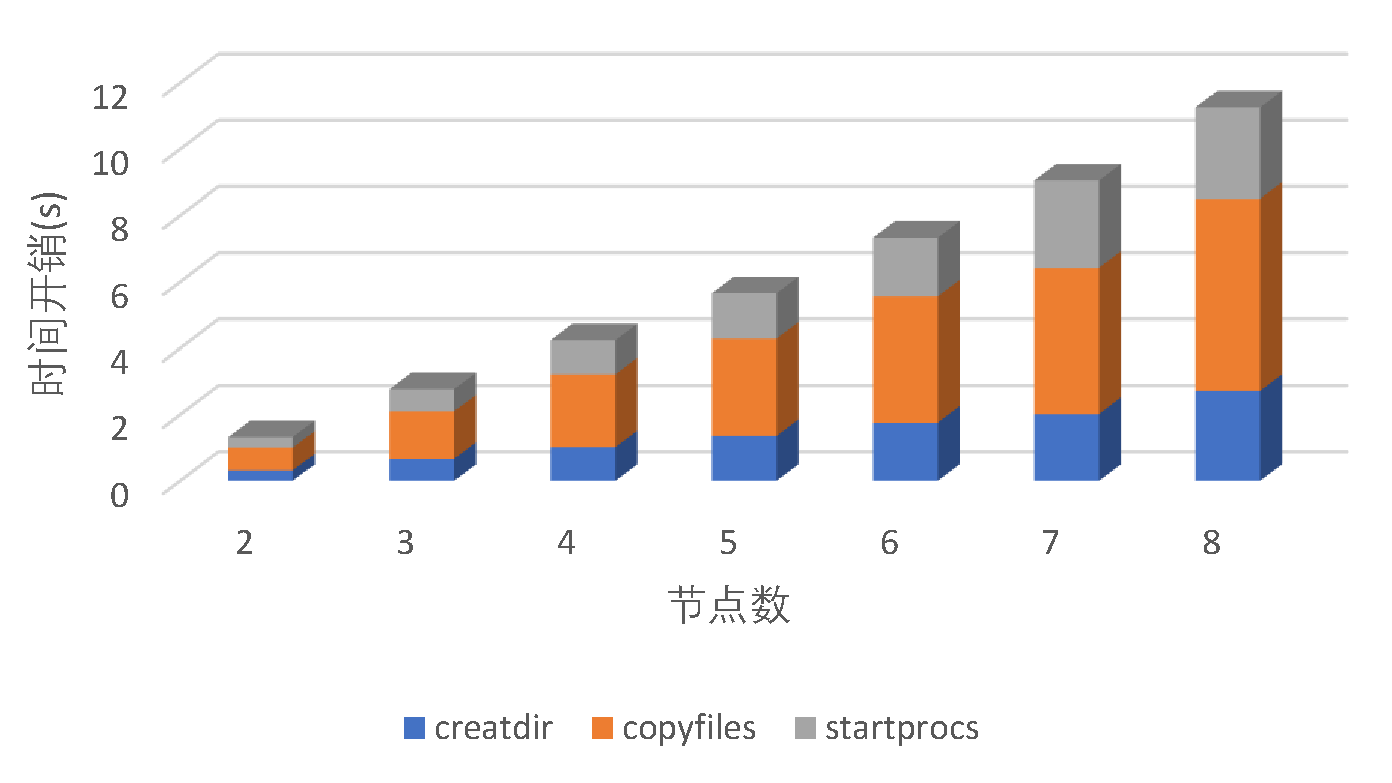
\includegraphics[width=0.85\linewidth]{Img/程序不同集群规模开销.pdf}
        \bicaption{\enspace 程序分发执行在不同集群规模下的开销}{\enspace Cost of Program Distribution and Launch with Varying Cluster Sizes}
        \label{fig:time-create-procs}
        {\footnotesize \par 注:测试在千兆以太网环境下进行,网络接口速度 1000 Mbps,采用 UDP 通信协议}
    \end{figure}

    \begin{figure}[!htbp]
        \centering
        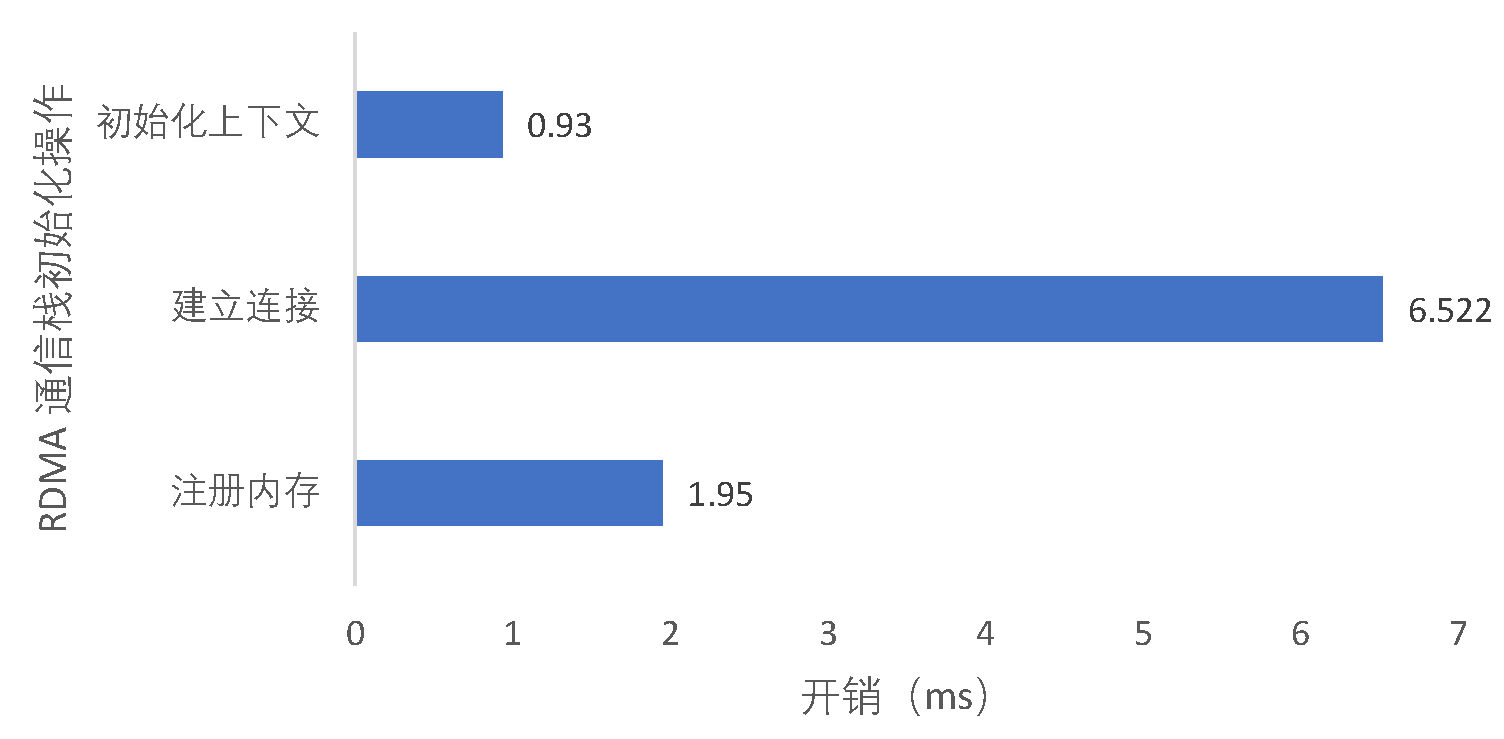
\includegraphics[width=0.85\linewidth]{Img/RDMA通信栈初始化开销分析.pdf}
        \bicaption{\enspace RDMA通信栈初始化开销分析}{\enspace RDMA Communication Stack Initialization Cost Analysis}
        \label{fig:time-init-rdma-comm}
        {\footnotesize \par 注:测试在两台配备 Mellanox ConnectX-3 Pro 网卡的工作站之间进行}
    \end{figure}

    \begin{figure}[!htbp]
        \centering
        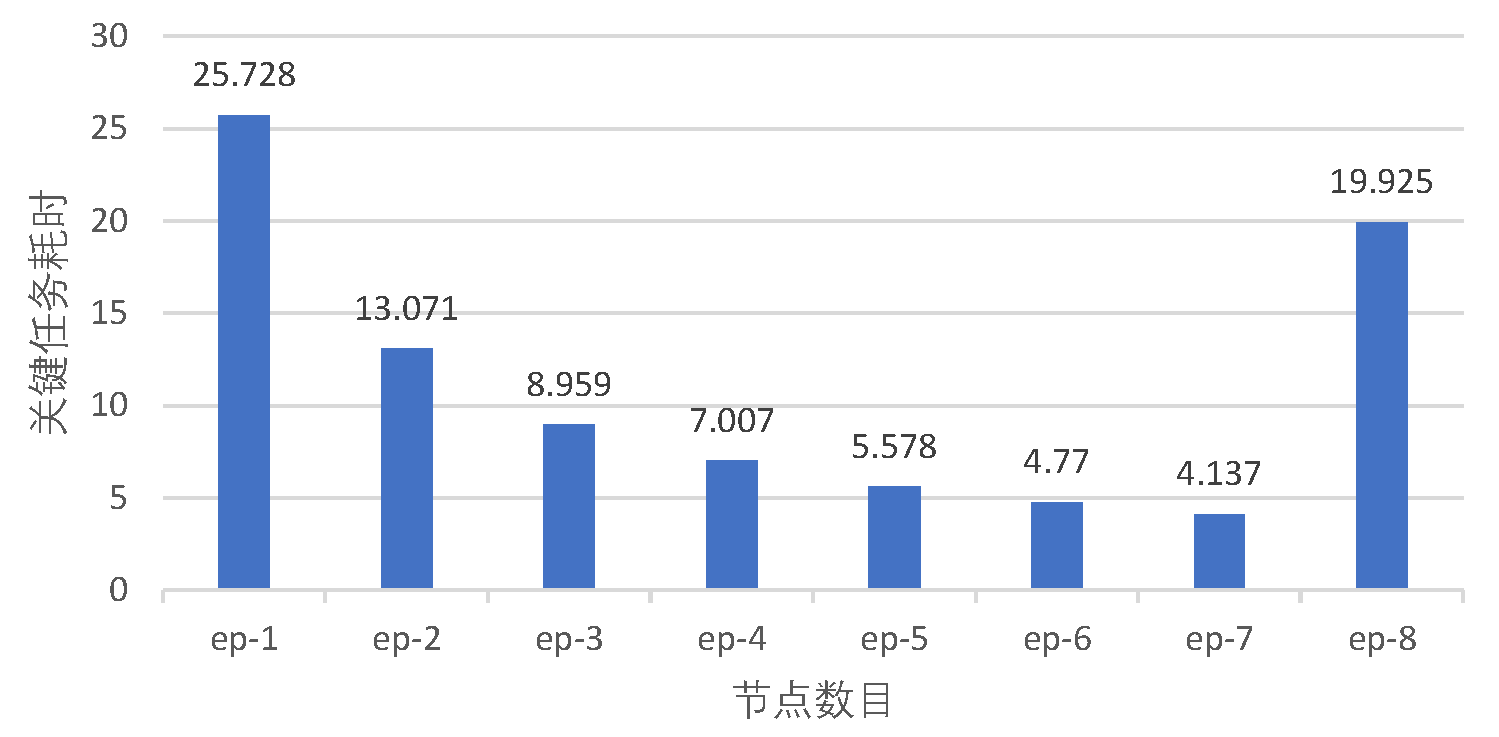
\includegraphics[width=\linewidth]{Img/EP-performance.pdf}
        \bicaption{\enspace 并行程序 ep 在不同节点数下的性能表现}{\enspace Parallel Program EP Performance on Varying Node Counts}
        \label{fig:ep-performance}
        {\footnotesize \par 注:测试在千兆以太网环境下进行,采用 UDP通信,
            测试节点1/2/3 搭载 Intel Xeon Gold 6338 CPU @ 2.000GHz 处理器,
            节点4/5/6搭载 Intel Xeon Platinum 8176 CPU @ 2.10GHz 处理器,
            节点 7 搭载AMD EPYC 9654 96-Core 处理器,
            节点 8 搭载AMD EPYC 9654 128-Core 处理器}
    \end{figure}

    \section{RDMA 通信栈 VS UDP 通信栈}\label{sec:通信栈}

    M-JIAJIA 系统的 UDP 和 RDMA 通信栈对比测试在两台戴尔 Precision 3660 塔式工作站之间进行。
    每台工作站配备 16 核第 12 代英特尔Core i9-12900K 处理器和 62.5GB 内存;UDP 通信栈通过千兆以太网进行数据传输,
    而 RDMA 通信栈依托 Mellanox ConnectX-3 Pro 网卡(最大带宽达 56000Mb/s),在 InfiniBand 模式下实现 RDMA 通信;
    测试程序依次是 water(288个分子)、lu($1024\times1024$)、ep($2^{28}$)、is($2^{22}$)、mm($1024\times1024$)、
    pi($10^6$个区间)、tsp(19个城市)、sor($256\times2048$)。

    图~\ref{fig:time-comparison-diff-stacks}显示了测试程序集在UDP、IPoIB与RDMA通信协议栈下执行的性能,
    横轴为各个测试程序,纵轴为主节点上程序运行时间,包含系统初始化开销。

    \begin{figure}[!htbp]
        \centering
        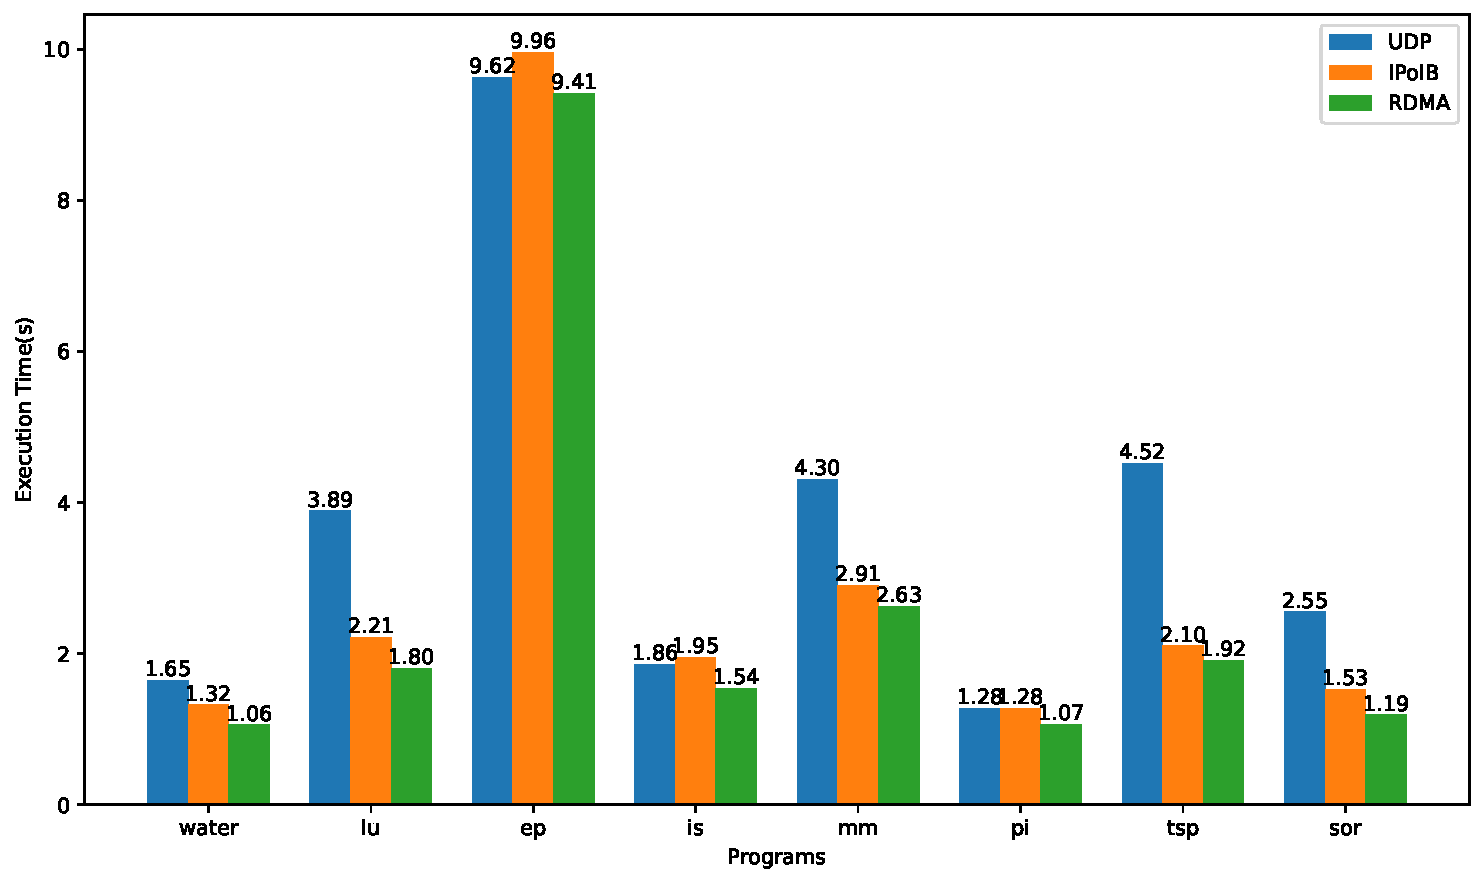
\includegraphics[width=\linewidth]{Img/execution_time_comparison.pdf}
        \bicaption{\enspace 不同通信栈下程序执行时间比较}{\enspace Comparison of Program Execution Time Across Different Communication Stacks}
        \label{fig:time-comparison-diff-stacks}
    \end{figure}

    结果表明,与 UDP 和 IPoIB 通信栈相比,RDMA 通信栈总是可以取得更优的性能。
    具体而言,相比于 UDP 通信栈下运行的程序,RDMA 通信栈下运行的程序性能分别提升了 water(35.94\%)、lu(53.71\%)、
    ep(2.16\%)、is(16.86\%)、mm(38.84\%)、pi(16.56\%)、tsp(57.52\%)与sor(53.39\%);
    相比于IPoIB,程序性能提升了  water(20.06\%)、lu(18.64\%)、
    ep(5.48\%)、is(21.00\%)、mm(9.49\%)、pi(16.48\%)、tsp(8.57\%)与sor(22.12\%)。
    这些程序性能提升差异的主要原因是程序的系统初始化开销、计算开销与通信开销占总开销的比例不同。

    部分程序性能的提升主要得益于同步开销的降低,这类程序通常不执行远程取页操作或仅在非主节点上执行远程取页操作,
    测试程序中的 water、ep、is与pi属于此类(如表~\ref{tab:type1-time}所示)。
    同步开销包括 barrier 和 lock 原语的执行时间,而其具体开销来源于请求同步变量(如锁或屏障)的成本以及传播 diffs 的开销。

    部分程序的性能提升主要体现在远程取页开销的降低上。
    这些程序包括 lu、mm 与 sor (详见表~\ref{tab:type2-time})。
    通过比较不同通信栈下相同数量远程取页的耗时差异,可以看出RDMA通信栈相较于UDP通信栈快了约18倍,相较于IPoIB快了2-3倍。
    同时,实验数据显示,本地访问一页触发段违例处理需要 4-5us,而在RDMA通信栈下远程访问一页触发段违例处理需要60-90us,这表明两者之间仍有一个数量级的差距。

    \begin{table}
        \footnotesize% fontsize
        \setlength{\tabcolsep}{4pt}% column separation
        \renewcommand{\arraystretch}{1.5}% row space 
        \centering
        \bicaption{不同通信栈下主节点部分程序的同步开销}{Synchronization Costs of Master Node Programs on Different Communication Stack}% caption
        \label{tab:type1-time}
        \begin{tabular}{l|c|c|c}
            \hline
            %\multicolumn{num_of_cols_to_merge}{alignment}{contents} \\
            %\cline{i-j}% partial hline from column i to column j
                        & Barrier 执行时间(个数) & Lock 执行时间(个数) & 同步时间(ms) \\
            \hline
            water-UDP   & 630.60 (35)      & 37.88 (35)    & 667.48   \\
            water-IPoIB & 322.26           & 4.85          & 327.11   \\
            water-RDMA  & 22.44            & 3.27          & 25.71    \\
            \hline
            ep-UDP      & 284.61 (3)       & 0.44 (1)      & 285.05   \\
            ep-IPoIB    & 285.60           & 0.44          & 286.04   \\
            ep-RDMA     & 4.23             & 0.30          & 4.53     \\
            \hline
            is-UDP      & 371.69 (32)      & 8.38 (10)     & 380.07   \\
            is-IPoIB    & 314.98           & 1.99          & 316.97   \\
            is-RDMA     & 8.65             & 0.94          & 9.59     \\
            \hline
            pi-UDP      & 289.88 (3)       & 5.88 (1)      & 295.76   \\
            pi-IPoIB    & 269.24           & 2.42          & 271.66   \\
            pi-RDMA     & 7.37             & 0.33          & 7.7      \\
            \hline
            tsp-UDP     & 3.31 (2)         & 2614.50 (380) & 2617.81  \\
            tsp-IPoIB   & 2.27             & 169.07        & 171.34   \\
            tsp-RDMA    & 0.84             & 43.82         & 44.66    \\
            \hline
        \end{tabular}
    \end{table}

    \begin{table}[!htbp]
        \footnotesize% fontsize
        \setlength{\tabcolsep}{4pt}% column separation
        \renewcommand{\arraystretch}{1.5}% row space 
        \centering
        \bicaption{不同通信栈下主节点部分程序的开销}{Costs of Master Node Programs on Different Communication Stack}% caption
        \label{tab:type2-time}
        \begin{tabular}{l|c|c|c|c}
            \hline
            %\multicolumn{num_of_cols_to_merge}{alignment}{contents} \\
            %\cline{i-j}% partial hline from column i to column j
                      & Barrier执行时间(个数) & 远程取页时间(页数)     & 通信总开销(ms) & 本地取页时间(页数)  \\
            \hline
            lu-UDP    & 938.25 (68)     & 818.11 (689)   & 1756.36   & 12.87(2770) \\
            lu-IPoIB  & 145.65          & 135.9          & 281.55    & 13.04       \\
            lu-RDMA   & 52.09           & 44.71          & 96.8      & 13.46       \\
            \hline
            mm-UDP    & 529.12 (3)      & 1277.84 (1024) & 1806.96   & 6.55(1536)  \\
            mm-IPoIB  & 319.11          & 144.5          & 463.61    & 7.02        \\
            mm-RDMA   & 19.74           & 69.31          & 89.05     & 6.29        \\
            \hline
            sor-UDP   & 496.48 (201)    & 325.31 (199)   & 821.79    & 1.38(324)   \\
            sor-IPoIB & 46.95           & 43.42          & 90.37     & 1.58        \\
            sor-RDMA  & 22.33           & 19.06          & 41.39     & 2.26        \\
            \hline
        \end{tabular}
    \end{table}

    \section{远程预取优化效果分析}\label{sec:远程预取优化效果分析}
    \begin{figure}[!htbp]
        \centering
        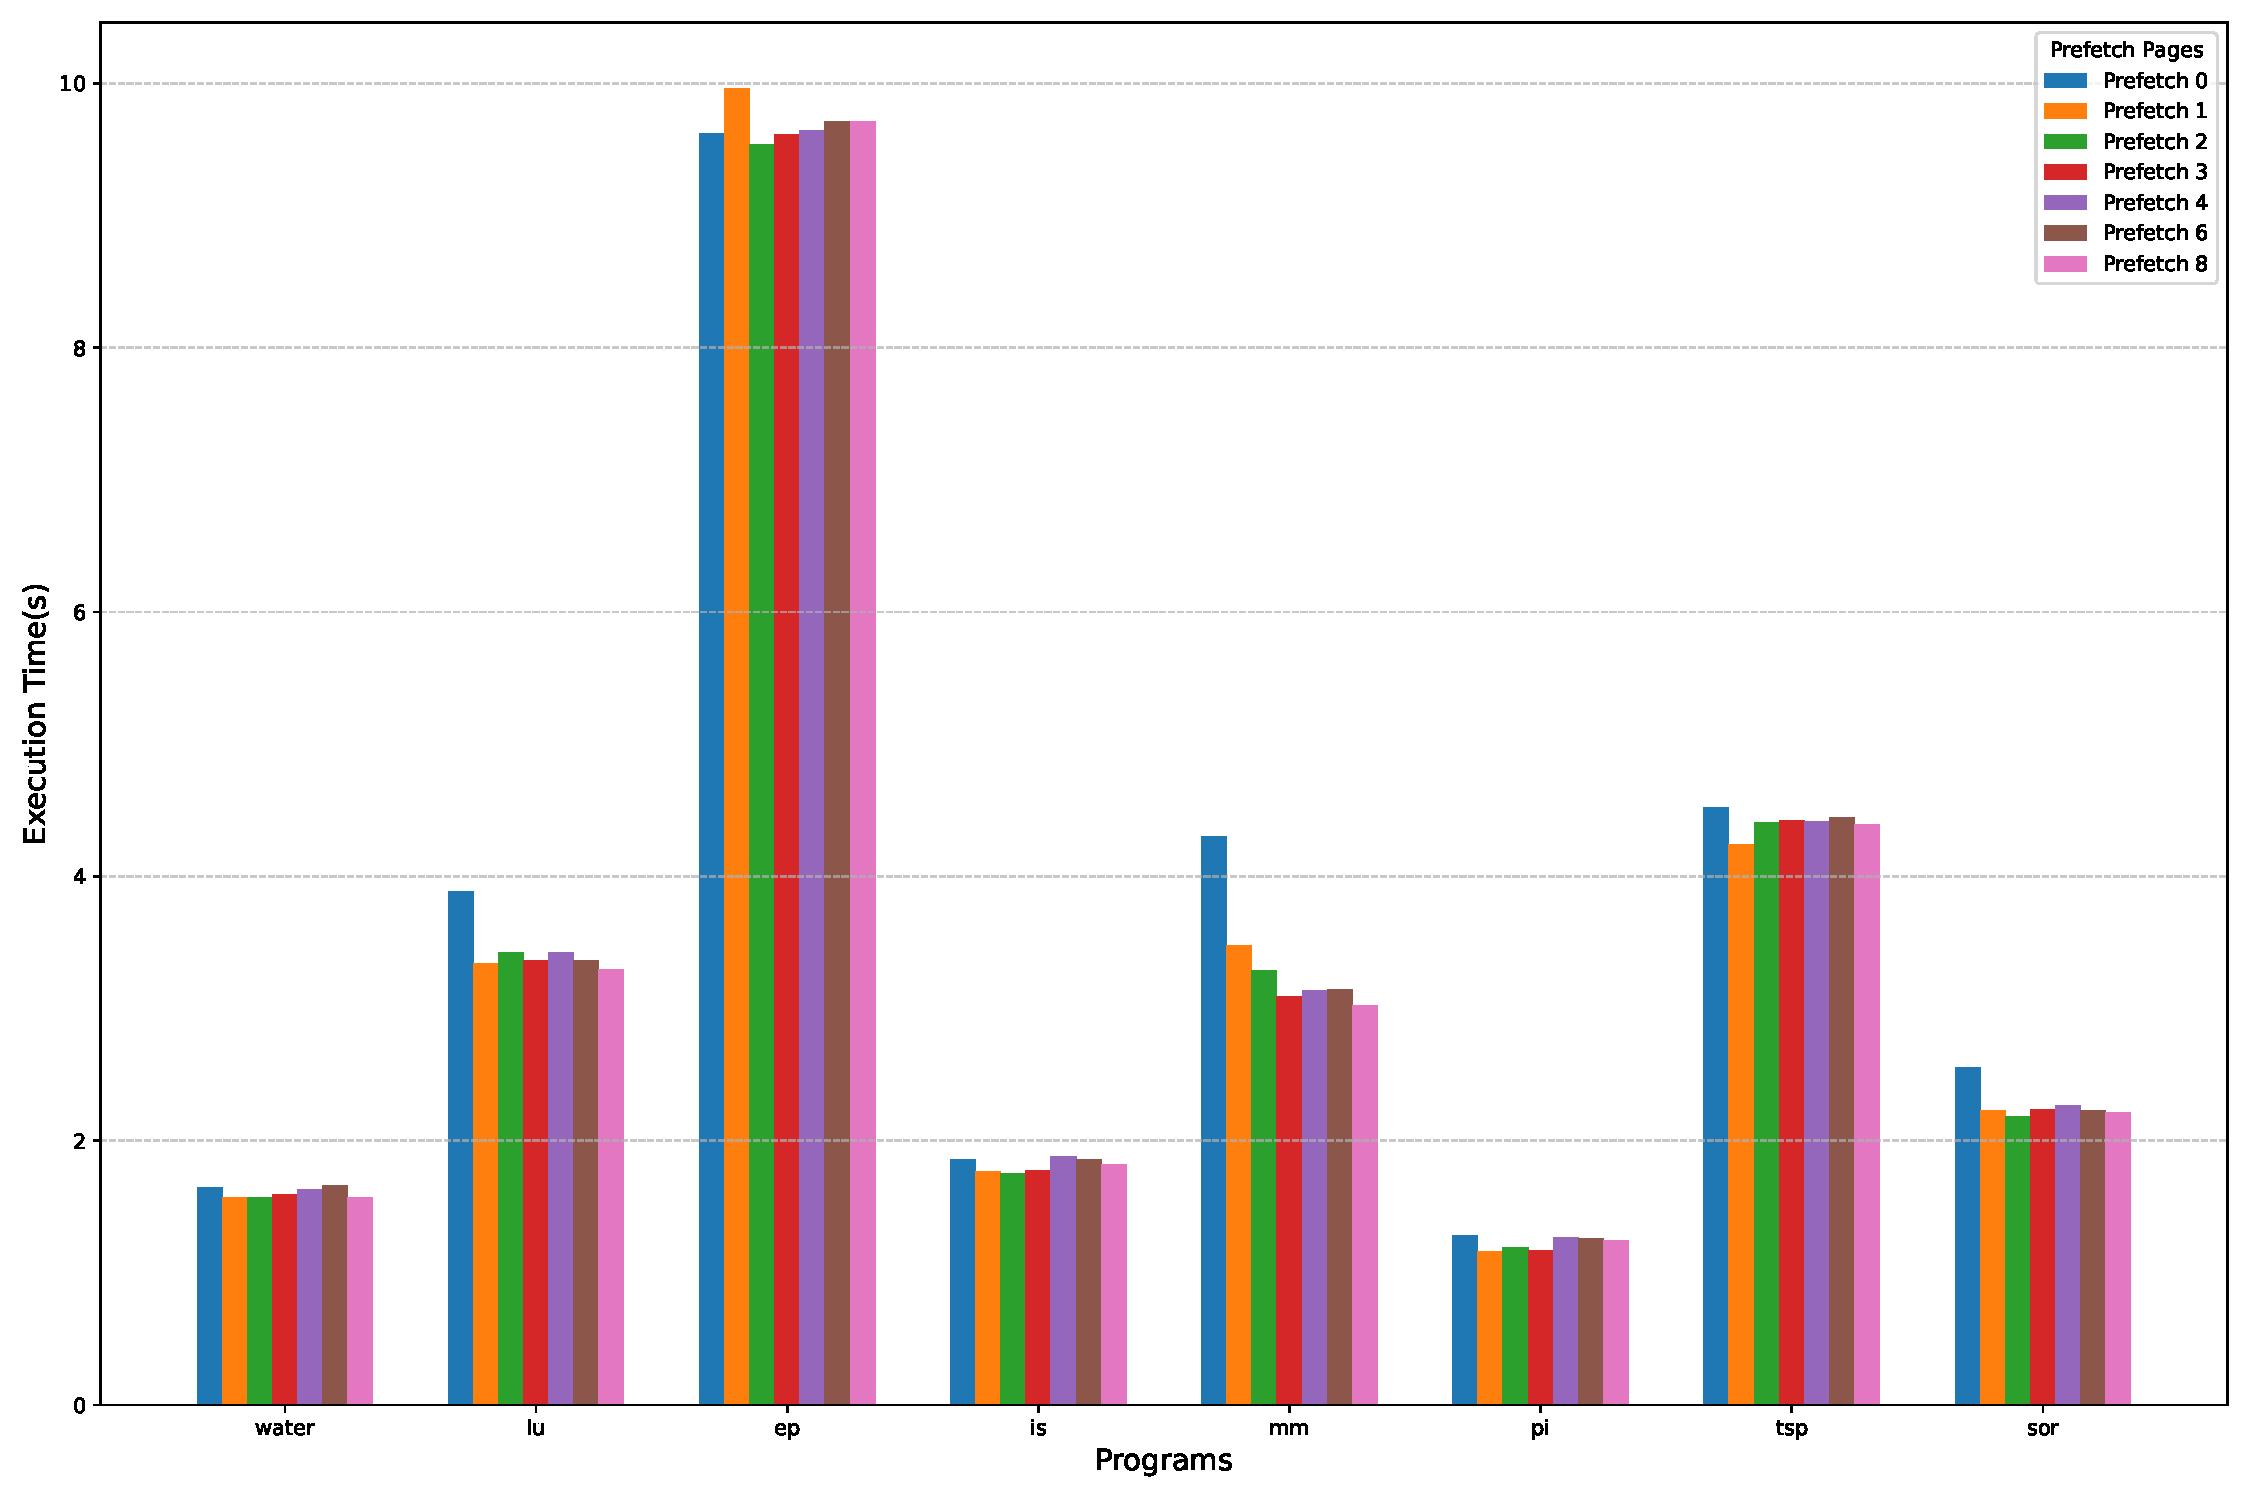
\includegraphics[width=0.90\linewidth]{Img/udp_prefetch_execution_time.pdf}
        \bicaption{UDP通信栈:程序性能与预取页数关系图}{UDP/IP Stack: Program Performance vs Prefetch Pages Relationship Diagram}
        \label{fig:udp-prefetch-result}
    \end{figure}
    图 ~\ref{fig:udp-prefetch-result} 展示了在 UDP 通信栈环境下,不同程序在不同预取页数条件下的执行性能表现。
    测试采用的环境与第 \ref{sec:通信栈}  小节中详述的 UDP 通信栈测试环境保持一致。
    实验结果表明,预取优化策略对多数程序的性能产生了显著影响。其中,lu、mm 和 sor 程序的性能提升尤为突出,分别实现了 13\%、41\% 和 12\% 的性能优化。
    分析原因是这些程序在运行过程中分配了较大规模的共享内存,预取机制发挥了关键作用,有效提升了整体性能。

    \begin{figure}
        \centering
        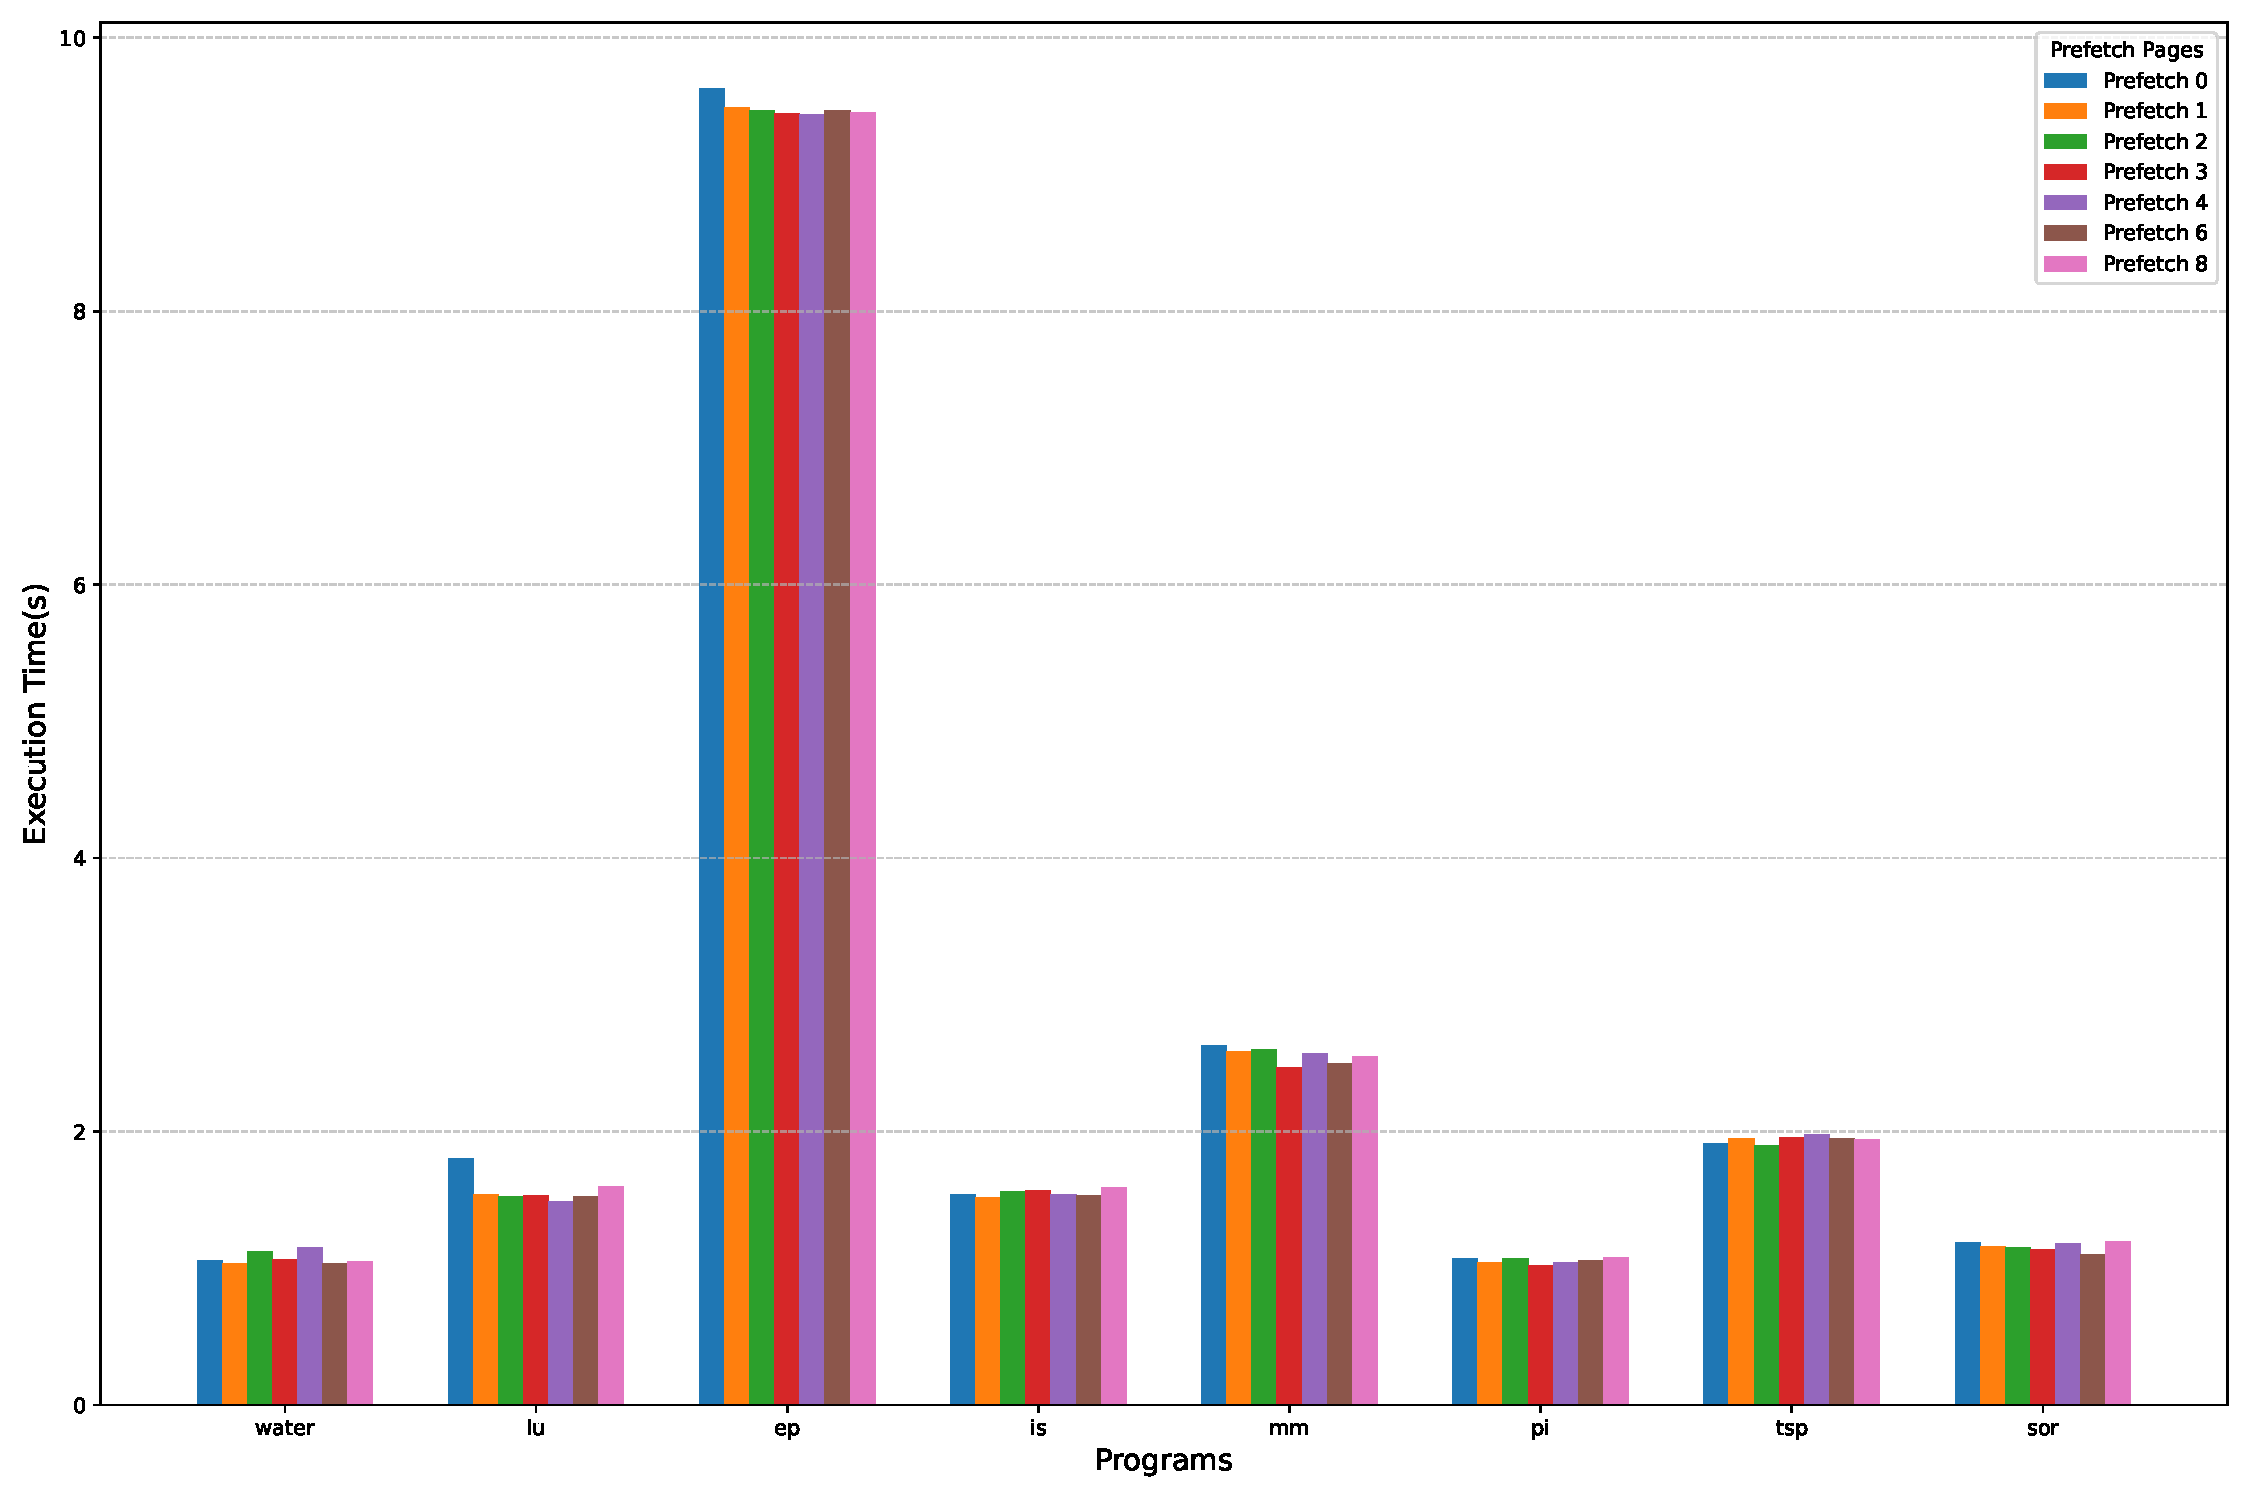
\includegraphics[width=0.90\linewidth]{Img/rdma_prefetch_execution_time.pdf}
        \bicaption{RDMA通信栈:程序性能与预取页数关系图}{RDMA Stack: Program Performance vs Prefetch Pages Relationship Diagram}
        \label{fig:rdma-prefetch-result}
    \end{figure}

    图~\ref{fig:rdma-prefetch-result} 展示了在 RDMA 通信栈环境下,不同程序在不同预取页数条件下的执行性能表现。
    测试采用的环境与第 \ref{sec:通信栈}  小节中详述的 RDMA 通信栈测试环境保持一致。
    实验结果表明,除了 lu 程序依旧可以获得较为明显的性能提升外,其余程序由于通信延迟的显著降低,预取优化的效果并不明显。
    分析原因是RDMA网络技术本身的传输性能已经很好,因此再进行预取优化对性能的影响并不显著。

    \section{类 MPI 接口测试}\label{sec:类 MPI 接口测试}
    M-JIAJIA 提供了类似于消息传递的基础通信接口 jia\_send 和 jia\_recv。
    图~\ref{fig:test-mpi} 展示了在不同通信栈下,这两个接口传输不同数据量时的性能表现,并与 OpenMPI 的 MPI\_send 和 MPI\_recv 在单机双进程间的性能进行了对比。
    测试环境与第 \ref{sec:通信栈} 小节中详细描述的 RDMA 通信栈测试环境保持一致,OpenMPI 的测试版本为 5.0.6。实验结果如下:

    \begin{figure}[!htbp]
        \centering
        \begin{subfigure}[b]{0.8\textwidth}
            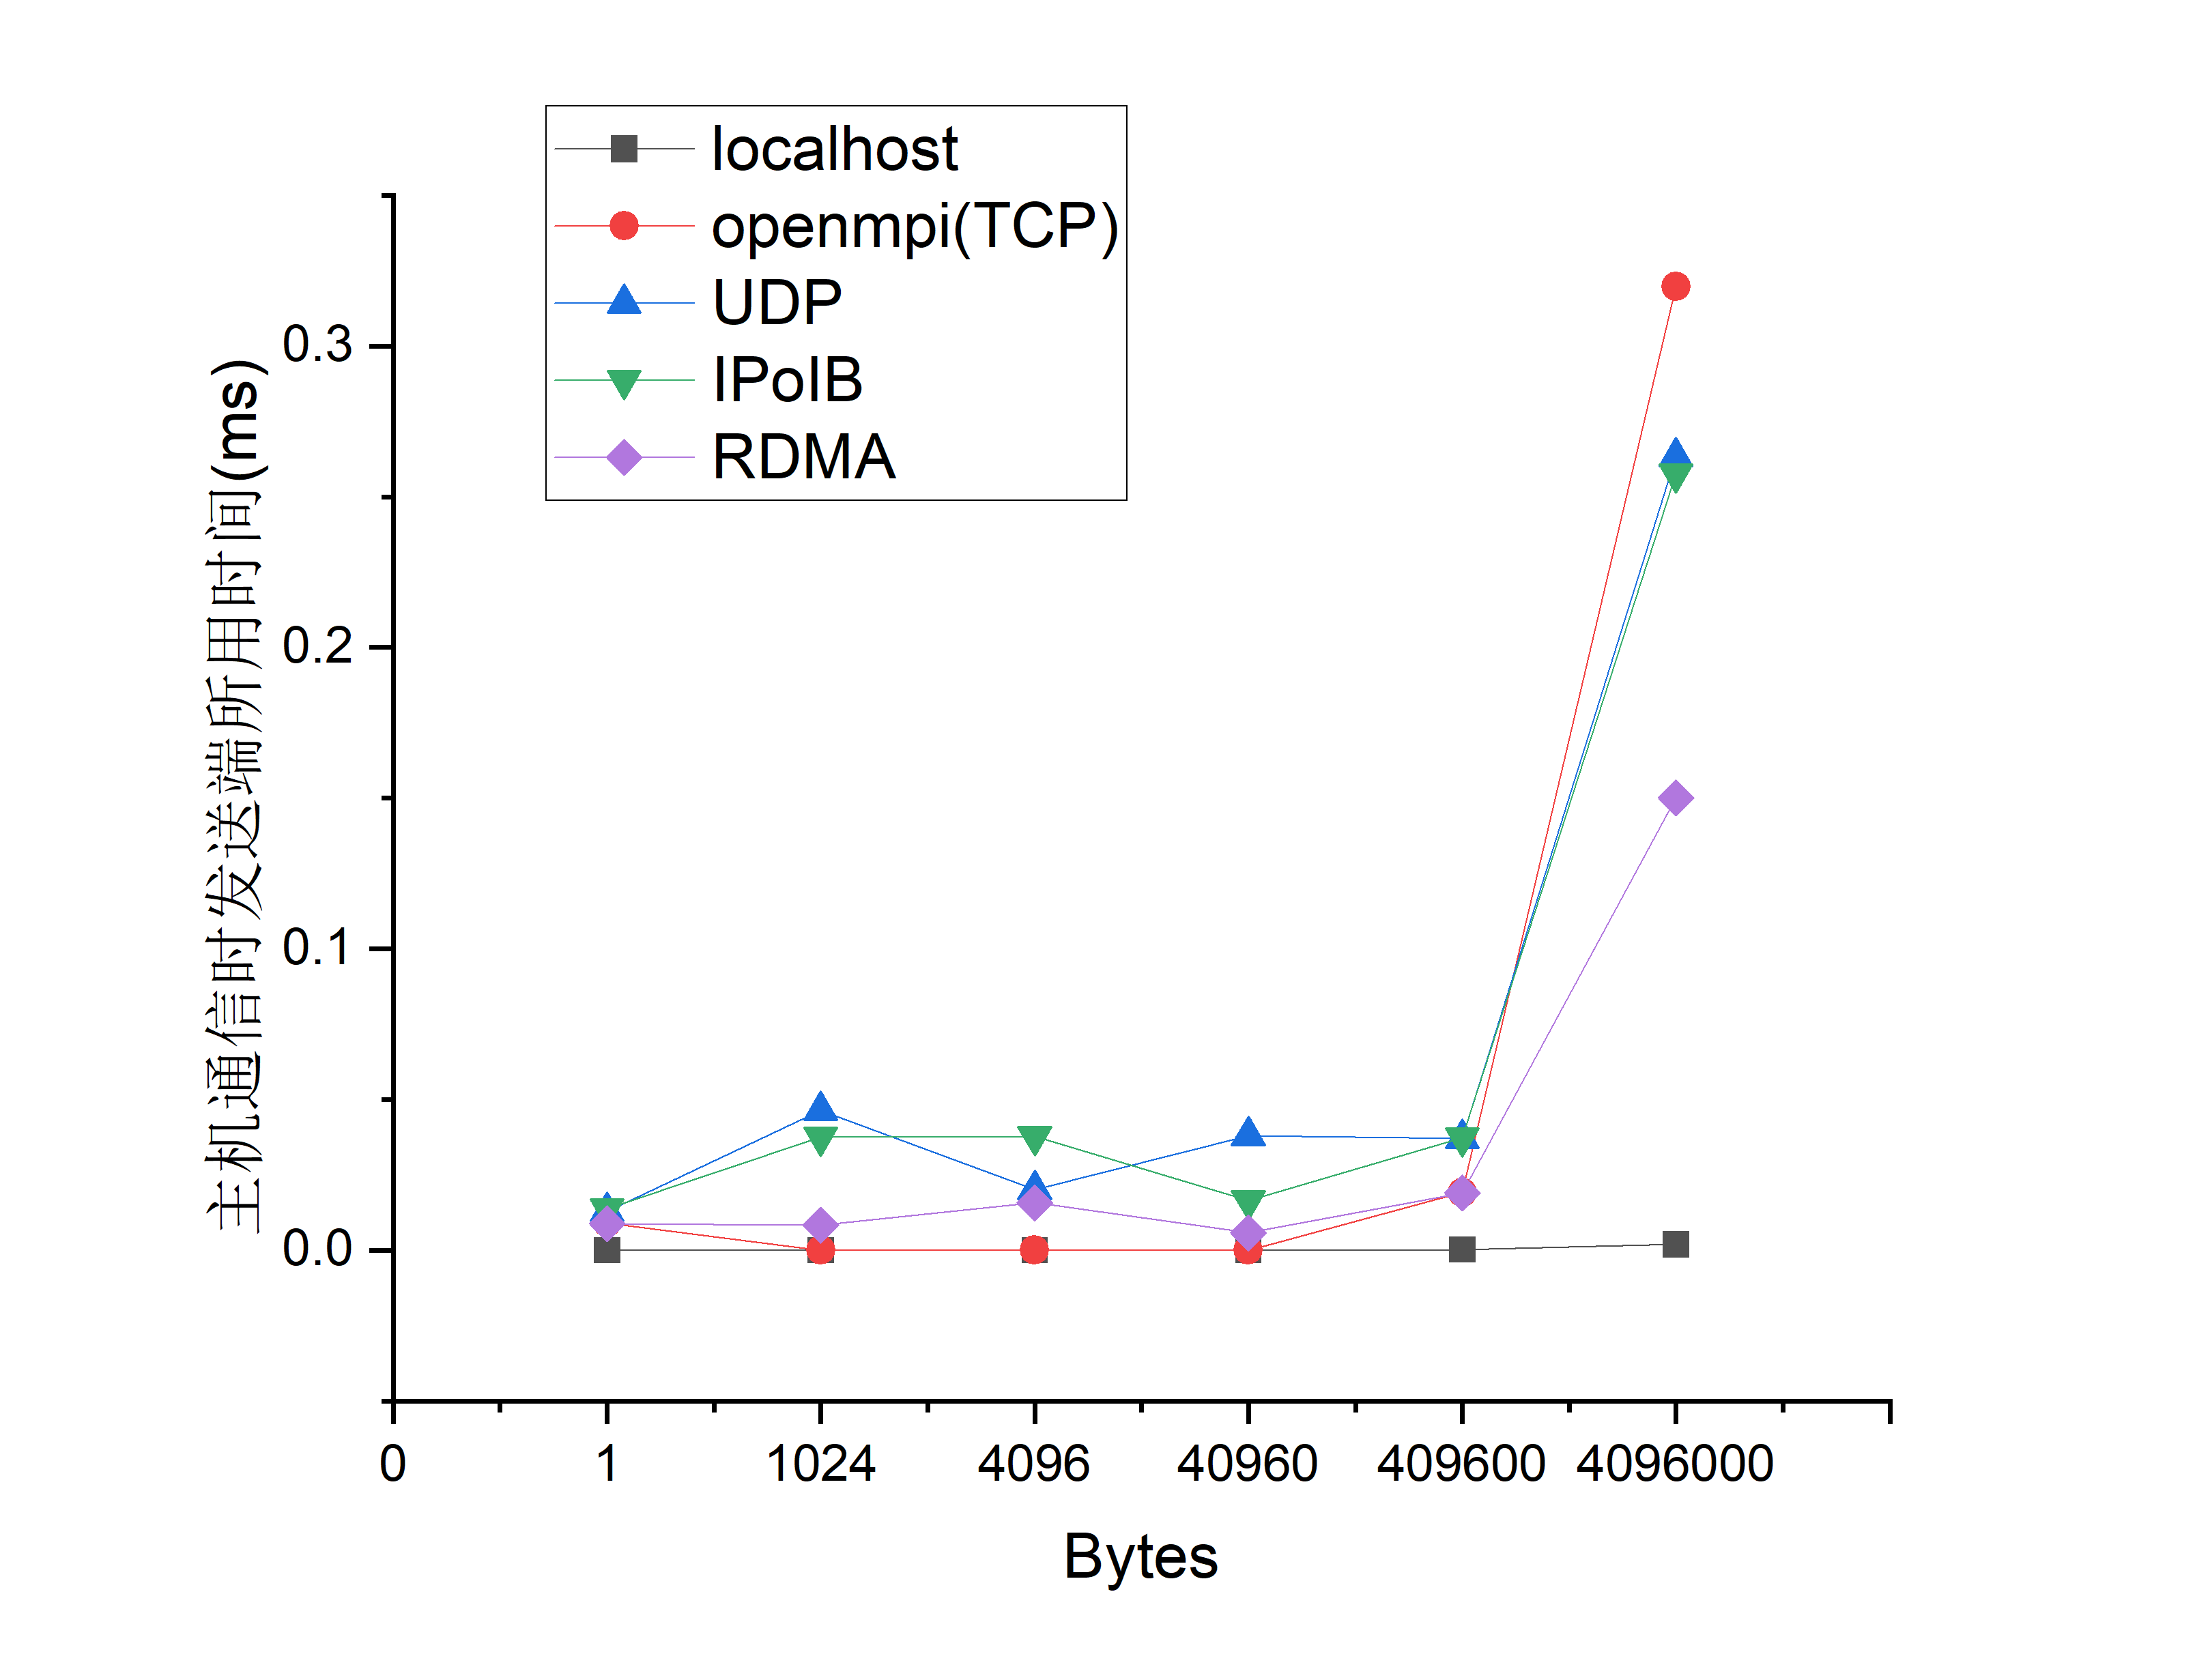
\includegraphics[width=1.0\textwidth]{Img/send_perf.png}
            \caption{jia\_send 接口性能测试}
            \label{fig:test-send}
        \end{subfigure}
        ~ % 添加期望的间隔
        \begin{subfigure}[b]{0.8\textwidth}
            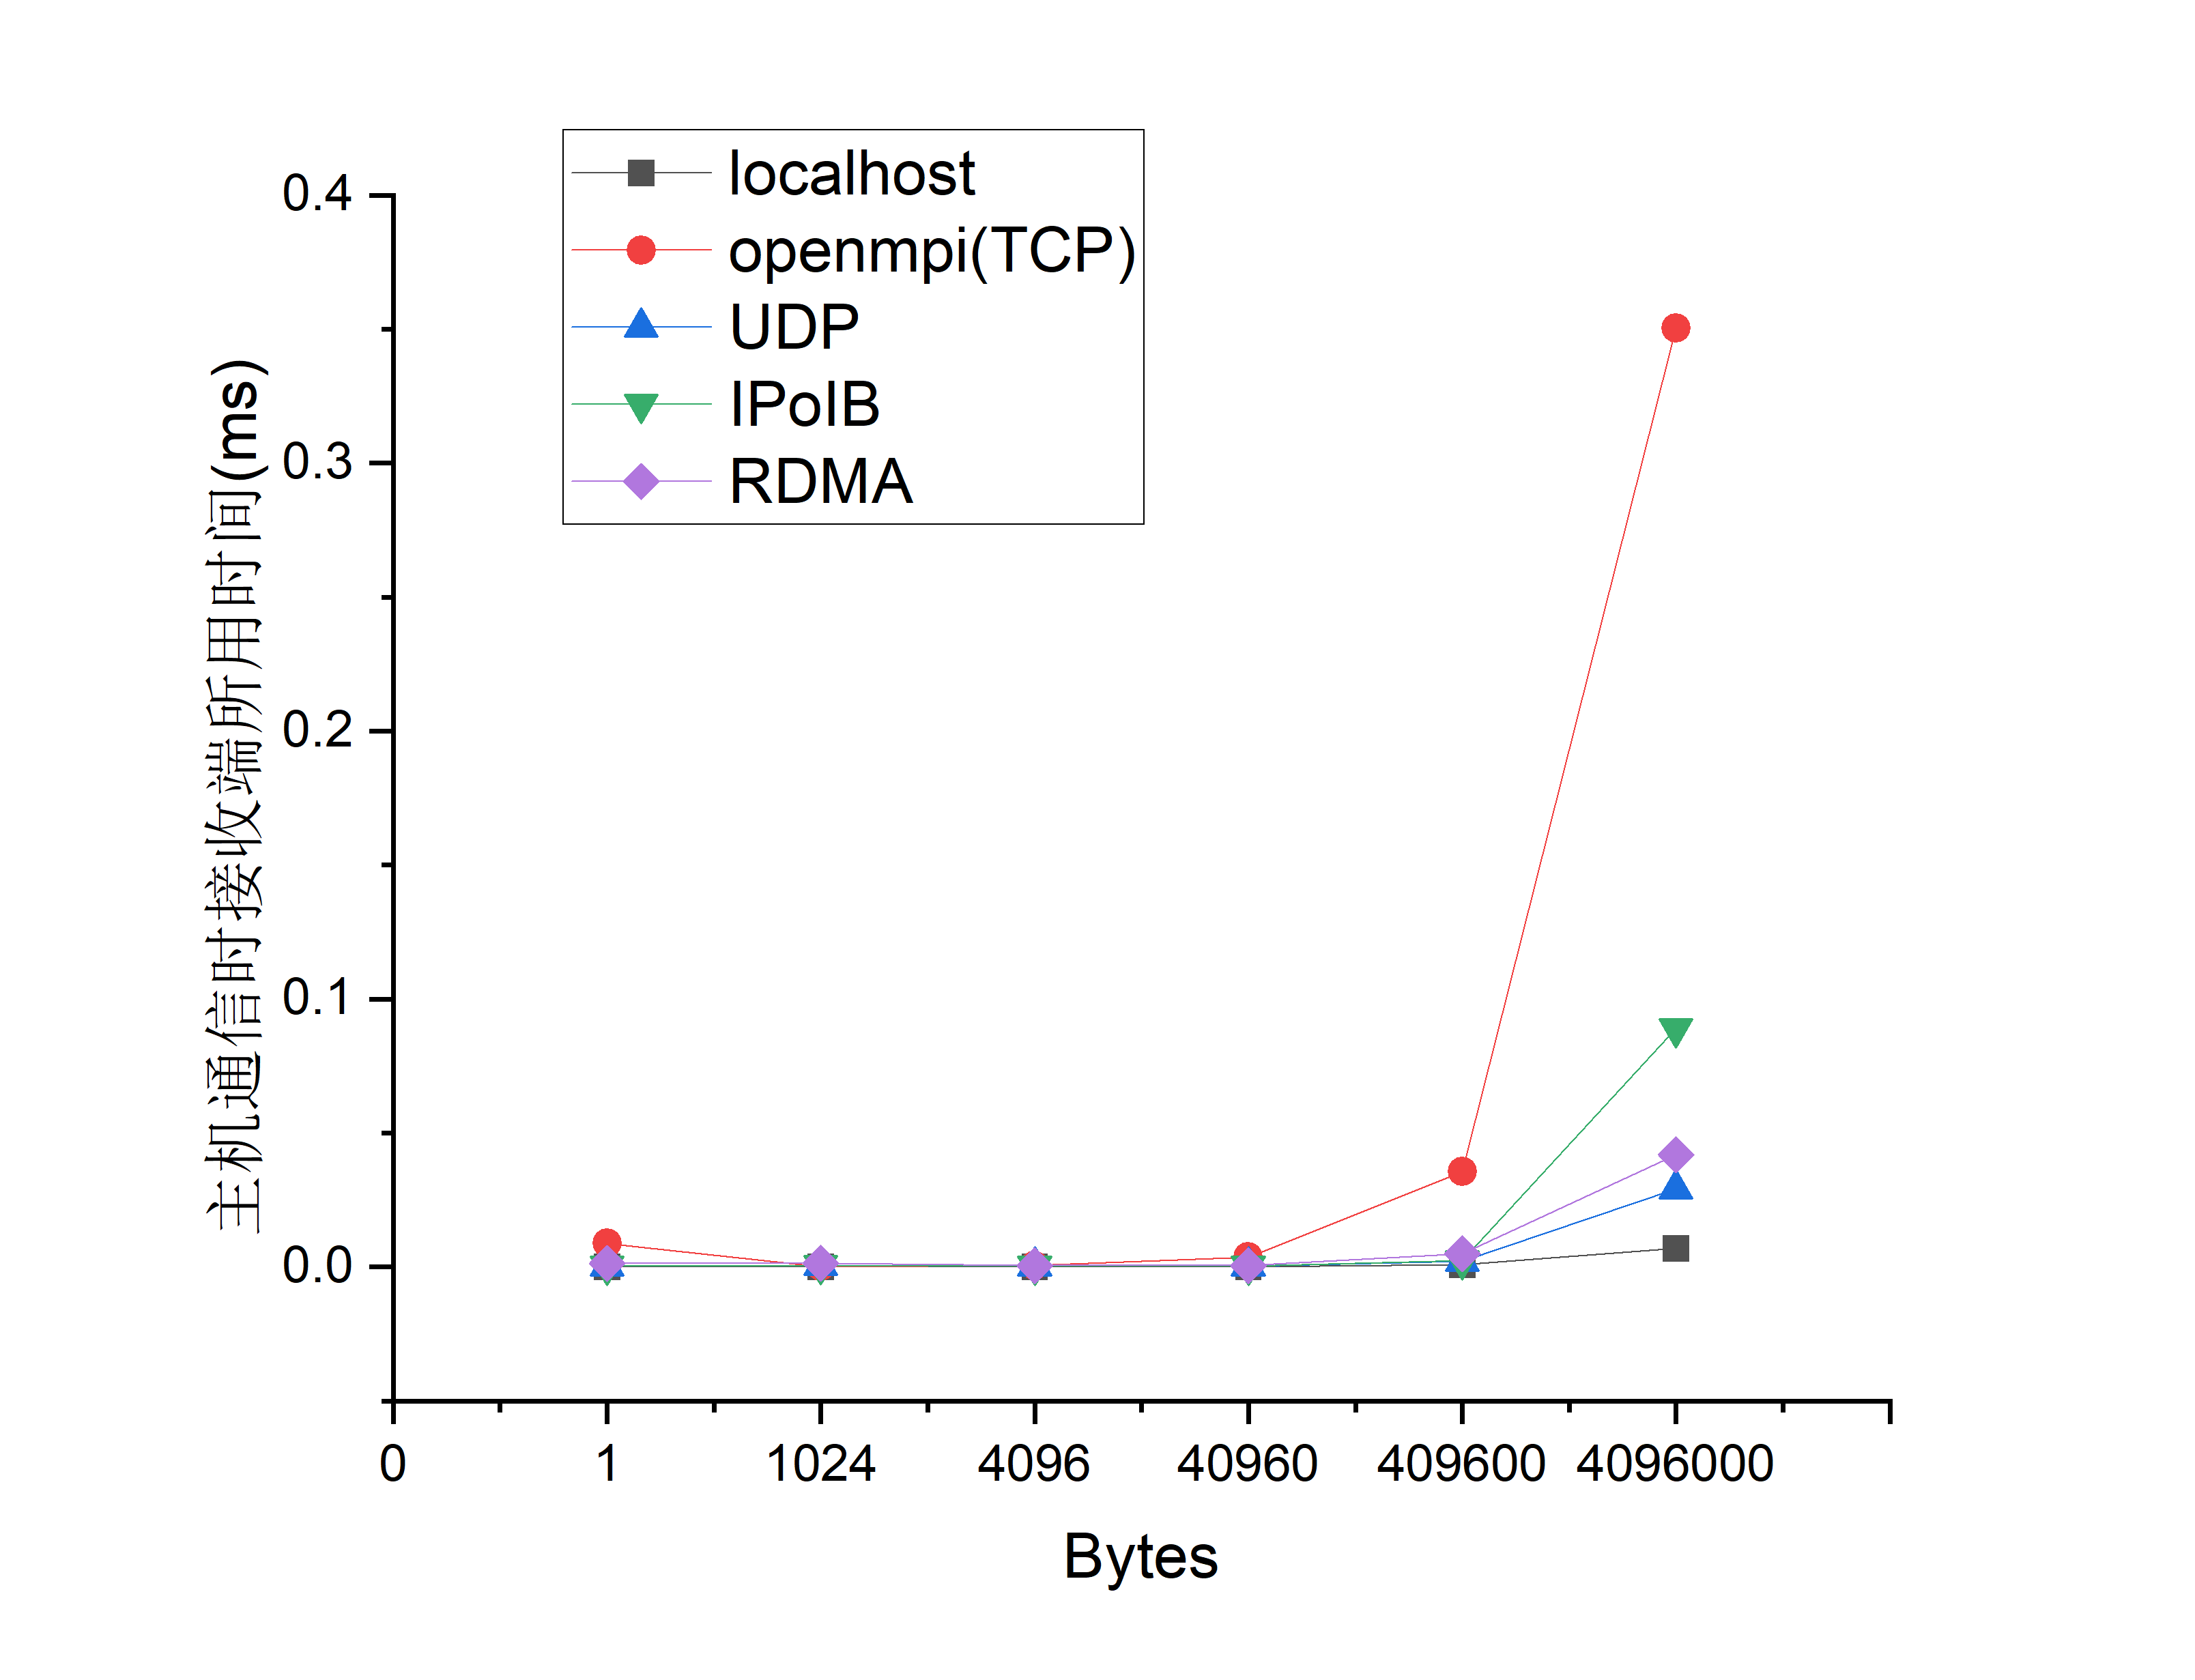
\includegraphics[width=1.0\textwidth]{Img/recv_perf.png}
            \caption{jia\_recv 接口性能测试}
            \label{fig:test-recv}
        \end{subfigure}
        \bicaption{\enspace 消息传递接口性能比较}{\enspace Performance Comparison of Message Passing Interfaces}
        \label{fig:test-mpi}
    \end{figure}

    由以上实验数据统计图可以看出:
    \begin{itemize}
        \item 接收端四种通信方式在小于40960字节时花费时间大致一致,大于40960字节时TCP连接花费时间显著多于另外三种连接花费时间;
              同时UDP,IPoIB与RDMA三种连接方式花费时间大致一致,没有显著区别;
        \item 发送端四种通信方式在小于409600字节时花费时间没有显著区别,波动属于正常区间;
              大于409600字节时TCP,UDP与IPoIB花费时间显著增长,明显多于RDMA发送端花费的时间(约为RDMA花费时间的2倍);
        \item 综合接收端与发送端所花费的时间可以看出,在大文件网络传输的情况下,TCP连接接收端与发送端花费时间均为最长(总时间最长);
              UDP与IPoIB网络连接总体花费时间大致一致,IpoIB在接收端花费的时间略长一些;RDMA连接花费的时间最短,且在发送端显著低于其他四种连接方式。
    \end{itemize}

    \section{本章小结}
    本章 \ref{sec:测试程序} 小节具体介绍 Water、LU、EP、IS、MM、PI、TSP和SOR 八个测试程序。

    本章 \ref{sec:程序开销分析} 小节将基于 M-JIAJIA 的程序开销细分为系统初始化开销、计算开销和通信开销三个部分,
    并探讨了系统初始化开销和计算开销的主要构成。

    本章 \ref{sec:通信栈} 小节主要比较了 UDP、IPoIB 和 RDMA 三种通信栈下测试程序的执行时间,
    并重点比较了RDMA相较UDP通信栈在性能上的提升,分析了性能提升与开销降低的关系。

    本章 \ref{sec:远程预取优化效果分析} 小节探讨了远程预取在 UDP 和 RDMA 通信栈中的优化效果。

    本章 \ref{sec:类 MPI 接口测试} 小节主要对比 UDP、IPoIB 和 RDMA 三种通信栈下M-JIAJIA类消息传递接口的性能,
    并与OpenMPI 单机多进程之间的消息传递性能进行了比较,重点比较了大字节传输时的性能提升。
}
\chapter{总结与展望}\label{chap:summary}{
    \section{本文工作总结}
    分布式共享内存作为一种重要的并行编程范式,在物理分布的系统上构建了一个逻辑上统一的地址空间。
    该范式融合了消息传递和共享内存的优点,不仅大大降低了分布式应用的开发复杂度,而且继承了分布式内存的高可扩展性。

    JIAJIA 是上世纪九十年代由计算技术研究所研发的国产软件 DSM 系统,
    基于域一致性内存模型的设计使得其在性能与编程复杂度之间获得良好的平衡,但由于网络技术不够成熟,导致实际运行时多节点通信往往成为整个系统的瓶颈。
    本文基于JIAJIA系统进行优化,开发出了M-JIAJIA系统。主要的优化有如下几点:
    \begin{enumerate}
        \item 重新进行UDP端口算法设计,并修改了多路复用机制与ack可靠通信机制,优化了UDP通信栈的构成;
        \item 将IO信号驱动单线程通信架构修改为了多线程通信架构,充分利用了硬件的性能;
        \item 分离通信层与核心逻辑层,使用循环消息队列作为两者之间的通信媒介,优化了系统的核心逻辑;
        \item 支持 UDP 和 RDMA 通信栈两种通信选择,利用RDMA网络技术,成功降低了系统的通信开销,提升了系统的性能。
    \end{enumerate}

    \section{未来研究方向}

    \begin{enumerate}
        \item RDMA read write 原语的进一步实现;
        \item jiajia对外接口扩展;
        \item 开发基于jiajia的分布式内存数据库;
        \item jiajia内存cache一致性模型的进一步扩展。
    \end{enumerate}
}
%---------------------------------------------------------------------------%
% main content

%-
%-> Appendix
%-

% \cleardoublepage %

\appendix% initialize the environment
\chapter{中国科学院大学学位论文撰写要求}

学位论文是研究生科研工作成果的集中体现,是评判学位申请者学术水平、授予其学位的主要依据,是科研领域重要的文献资料。根据《科学技术报告、学位论文和学术论文的编写格式》(GB/T 7713-1987)、《学位论文编写规则》(GB/T 7713.1-2006)和《文后参考文献著录规则》(GB7714—87)等国家有关标准,结合中国科学院大学(以下简称“国科大”)的实际情况,特制订本规定。

\section{论文无附录者无需附录部分}

\section{测试公式编号 \texorpdfstring{$\Lambda,\lambda,\theta,\bar{\Lambda},\sqrt{S_{NN}}$}{$\textLambda,\textlambda,\texttheta,\bar{\textLambda},\sqrt{S_{NN}}$}} \label{sec:testmath}

\begin{equation} \label{eq:appedns}
    \adddotsbeforeeqnnum%
    \begin{cases}
        \frac{\partial \rho}{\partial t} + \nabla\cdot(\rho\Vector{V}) = 0\\
        \frac{\partial (\rho\Vector{V})}{\partial t} + \nabla\cdot(\rho\Vector{V}\Vector{V}) = \nabla\cdot\Tensor{\sigma}\\
        \frac{\partial (\rho E)}{\partial t} + \nabla\cdot(\rho E\Vector{V}) = \nabla\cdot(k\nabla T) + \nabla\cdot(\Tensor{\sigma}\cdot\Vector{V})
    \end{cases}
\end{equation}
\begin{equation}
    \adddotsbeforeeqnnum%
    \frac{\partial }{\partial t}\int\limits_{\Omega} u \, \mathrm{d}\Omega + \int\limits_{S} \unitVector{n}\cdot(u\Vector{V}) \, \mathrm{d}S = \dot{\phi}
\end{equation}
\[
    \begin{split}
        \mathcal{L} \{f\}(s) &= \int _{0^{-}}^{\infty} f(t) e^{-st} \, \mathrm{d}t, \ 
        \mathscr{L} \{f\}(s) = \int _{0^{-}}^{\infty} f(t) e^{-st} \, \mathrm{d}t\\
        \mathcal{F} {\bigl (} f(x+x_{0}) {\bigr )} &= \mathcal{F} {\bigl (} f(x) {\bigr )} e^{2\pi i\xi x_{0}}, \ 
        \mathscr{F} {\bigl (} f(x+x_{0}) {\bigr )} = \mathscr{F} {\bigl (} f(x) {\bigr )} e^{2\pi i\xi x_{0}}
    \end{split}
\]

mathtext: $A,F,L,2,3,5,\sigma$, mathnormal: $A,F,L,2,3,5,\sigma$, mathrm: $\mathrm{A,F,L,2,3,5,\sigma}$.

mathbf: $\mathbf{A,F,L,2,3,5,\sigma}$, mathit: $\mathit{A,F,L,2,3,5,\sigma}$, mathsf: $\mathsf{A,F,L,2,3,5,\sigma}$.

mathtt: $\mathtt{A,F,L,2,3,5,\sigma}$, mathfrak: $\mathfrak{A,F,L,2,3,5,\sigma}$, mathbb: $\mathbb{A,F,L,2,3,5,\sigma}$.

mathcal: $\mathcal{A,F,L,2,3,5,\sigma}$, mathscr: $\mathscr{A,F,L,2,3,5,\sigma}$, boldsymbol: $\boldsymbol{A,F,L,2,3,5,\sigma}$.

vector: $\Vector{\sigma, T, a, F, n}$, unitvector: $\unitVector{\sigma, T, a, F, n}$

matrix: $\Matrix{\sigma, T, a, F, n}$, unitmatrix: $\unitMatrix{\sigma, T, a, F, n}$

tensor: $\Tensor{\sigma, T, a, F, n}$, unittensor: $\unitTensor{\sigma, T, a, F, n}$ 

\section{测试生僻字}

霜蟾盥薇曜灵霜颸妙鬘虚霩淩澌菀枯菡萏泬寥窅冥毰毸濩落霅霅便嬛岧峣瀺灂姽婳愔嫕飒纚棽俪緸冤莩甲摛藻卮言倥侗椒觞期颐夜阑彬蔚倥偬澄廓簪缨陟遐迤逦缥缃鹣鲽憯懔闺闼璀错媕婀噌吰澒洞阛闠覼缕玓瓑逡巡諓諓琭琭瀌瀌踽踽叆叇氤氲瓠犀流眄蹀躞赟嬛茕頔璎珞螓首蘅皋惏悷缱绻昶皴皱颟顸愀然菡萏卑陬纯懿犇麤掱暒 墌墍墎墏墐墒墒墓墔墕墖墘墖墚墛坠墝增墠墡墢墣墤墥墦墧墨墩墪樽墬墭堕墯墰墱墲坟墴墵垯墷墸墹墺墙墼墽垦墿壀壁壂壃壄壅壆坛壈壉壊垱壌壍埙壏壐壑壒压壔壕壖壗垒圹垆壛壜壝垄壠壡坜壣壤壥壦壧壨坝塆圭嫶嫷嫸嫹嫺娴嫼嫽嫾婳妫嬁嬂嬃嬄嬅嬆嬇娆嬉嬊娇嬍嬎嬏嬐嬑嬒嬓嬔嬕嬖嬗嬘嫱嬚嬛嬜嬞嬟嬠嫒嬢嬣嬥嬦嬧嬨嬩嫔嬫嬬奶嬬嬮嬯婴嬱嬲嬳嬴嬵嬶嬷婶嬹嬺嬻嬼嬽嬾嬿孀孁孂娘孄孅孆孇孆孈孉孊娈孋孊孍孎孏嫫婿媚嵭嵮嵯嵰嵱嵲嵳嵴嵵嵶嵷嵸嵹嵺嵻嵼嵽嵾嵿嶀嵝嶂嶃崭嶅嶆岖嶈嶉嶊嶋嶌嶍嶎嶏嶐嶑嶒嶓嵚嶕嶖嶘嶙嶚嶛嶜嶝嶞嶟峤嶡峣嶣嶤嶥嶦峄峃嶩嶪嶫嶬嶭崄嶯嶰嶱嶲嶳岙嶵嶶嶷嵘嶹岭嶻屿岳帋巀巁巂巃巄巅巆巇巈巉巊岿巌巍巎巏巐巑峦巓巅巕岩巗巘巙巚帠帡帢帣帤帨帩帪帬帯帰帱帲帴帵帷帹帺帻帼帽帾帿幁幂帏幄幅幆幇幈幉幊幋幌幍幎幏幐幑幒幓幖幙幚幛幜幝幞帜幠幡幢幤幥幦幧幨幩幪幭幮幯幰幱庍庎庑庖庘庛庝庠庡庢庣庤庥庨庩庪庬庮庯庰庱庲庳庴庵庹庺庻庼庽庿廀厕廃厩廅廆廇廋廌廍庼廏廐廑廒廔廕廖廗廘廙廛廜廞庑廤廥廦廧廨廭廮廯廰痈廲廵廸廹廻廼廽廿弁弅弆弇弉弖弙弚弜弝弞弡弢弣弤弨弩弪弫弬弭弮弰弲弪弴弶弸弻弼弽弿彖彗彘彚彛彜彝彞彟彴彵彶彷彸役彺彻彽彾佛徂徃徆徇徉后徍徎徏径徒従徔徕徖徙徚徛徜徝从徟徕御徢徣徤徥徦徧徨复循徫旁徭微徯徰徱徲徳徴徵徶德徸彻徺忁忂惔愔忇忈忉忔忕忖忚忛応忝忞忟忪挣挦挧挨挩挪挫挬挭挮挰掇授掉掊掋掍掎掐掑排掓掔掕挜掚挂掜掝掞掟掠采探掣掤掦措掫掬掭掮掯掰掱掲掳掴掵掶掸掹掺掻掼掽掾掿拣揁揂揃揅揄揆揇揈揉揊揋揌揍揎揑揓揔揕揖揗揘揙揤揥揦揧揨揫捂揰揱揲揳援揵揶揷揸揻揼揾揿搀搁搂搃搄搅搇搈搉搊搋搌搎搏搐搑搒摓摔摕摖摗摙摚摛掼摝摞摠摡斫斩斮斱斲斳斴斵斶斸旪旫旮旯晒晓晔晕晖晗晘晙晛晜晞晟晠晡晰晣晤晥晦晧晪晫晬晭晰晱晲晳晴晵晷晸晹晻晼晽晾晿暀暁暂暃暄暅暆暇晕晖暊暋暌暍暎暏暐暑暒暓暔暕暖暗旸暙暚暛暜暝暞暟暠暡暣暤暥暦暧暨暩暪暬暭暮暯暰昵暲暳暴暵
% appendix content

%-
%-> Backmatter: bibliography, glossary, index
%-

\intotoc*{\cleardoublepage}{\bibname}% add link to toc
% \bibliographystyle{elsarticle-num}
\artxifstreq{\artxbib}{bibtex}{% enable bibtex
    \bibliography{Biblio/ref}% bibliography
}{%
    \printbibliography% bibliography
}
\cleardoublepage

\backmatter% initialize the environment
%---------------------------------------------------------------------------%
%->> Backmatter
%---------------------------------------------------------------------------%
\chapter[致谢]{致\quad 谢}\chaptermark{致\quad 谢}% syntax: \chapter[目录]{标题}\chaptermark{页眉}
%\thispagestyle{noheaderstyle}% 如果需要移除当前页的页眉
%\pagestyle{noheaderstyle}% 如果需要移除整章的页眉

感激casthesis作者吴凌云学长,gbt7714-bibtex-style
开发者zepinglee,和ctex众多开发者们。若没有他们的辛勤付出和非凡工作,\LaTeX{}菜鸟的我是无法完成此国科大学位论文\LaTeX{}模板ucasthesis的。在\LaTeX{}中的一点一滴的成长源于开源社区的众多优秀资料和教程,在此对所有\LaTeX{}社区的贡献者表示感谢!

ucasthesis国科大学位论文\LaTeX{}模板的最终成型离不开以霍明虹老师和丁云云老师为代表的国科大学位办公室老师们制定的官方指导文件和众多ucasthesis用户的热心测试和耐心反馈,在此对他们的认真付出表示感谢。特别对国科大的赵永明同学的众多有效反馈意见和建议表示感谢,对国科大本科部的陆晴老师和本科部学位办的丁云云老师的细致审核和建议表示感谢。谢谢大家的共同努力和支持,让ucasthesis为国科大学子使用\LaTeX{}撰写学位论文提供便利和高效这一目标成为可能。

\chapter{作者简历及攻读学位期间发表的学术论文与研究成果}

\textbf{本科生无需此部分}。

\section*{作者简历:}

\subsection*{casthesis作者}

吴凌云,福建省屏南县人,中国科学院数学与系统科学研究院博士研究生。

\subsection*{ucasthesis作者}

莫晃锐,湖南省湘潭县人,中国科学院力学研究所硕士研究生。

\section*{已发表(或正式接受)的学术论文:}

 {
  \setlist[enumerate]{}% restore default behavior
  \begin{enumerate}[nosep]
      \item ucasthesis: A LaTeX Thesis Template for the University of Chinese Academy of Sciences, 2014.
  \end{enumerate}
 }

\section*{申请或已获得的专利:}

(无专利时此项不必列出)

\section*{参加的研究项目及获奖情况:}

可以随意添加新的条目或是结构。

\cleardoublepage[plain]% 让文档总是结束于偶数页,可根据需要设定页眉页脚样式,如 [noheaderstyle]
%---------------------------------------------------------------------------%
% other information

\nocite{*}  % 使 ref.bib 中的文件都出现在参考文献列表中

\end{document}
%---------------------------------------------------------------------------%

